\documentclass[journal, twoside]{IEEEtran}

% *** self loaded ***
% \usepackage[euler]{textgreek} % greek letters (for \textmu), not in use now
\usepackage{cite}
\usepackage{url}
\usepackage{multirow}
\usepackage{xcolor}
\usepackage[range-units = single, range-phrase = --, detect-all, per-mode = symbol, binary-units=true]{siunitx}
\usepackage{enumitem}
% \usepackage{soul}


% *** GRAPHICS RELATED PACKAGES ***
%
\ifCLASSINFOpdf
    \usepackage[pdftex]{graphicx}
    \graphicspath{{figure/}}
    \DeclareGraphicsExtensions{.pdf,.jpeg,.png}
\else
  % or other class option (dvipsone, dvipdf, if not using dvips). graphicx
  % will default to the driver specified in the system graphics.cfg if no
  % driver is specified.
  % \usepackage[dvips]{graphicx}
  % declare the path(s) where your graphic files are
  % \graphicspath{{../eps/}}
  % and their extensions so you won't have to specify these with
  % every instance of \includegraphics
  % \DeclareGraphicsExtensions{.eps}
\fi


% *** MATH PACKAGES ***
%
\usepackage{amsmath}
% A popular package from the American Mathematical Society that provides
% many useful and powerful commands for dealing with mathematics.
%
% Note that the amsmath package sets \interdisplaylinepenalty to 10000
% thus preventing page breaks from occurring within multiline equations. Use:
\interdisplaylinepenalty=2500
% after loading amsmath to restore such page breaks as IEEEtran.cls normally
% does. amsmath.sty is already installed on most LaTeX systems. The latest
% version and documentation can be obtained at:
% http://www.ctan.org/pkg/amsmath


% *** SPECIALIZED LIST PACKAGES ***
\usepackage{algorithmic}

% *** ALIGNMENT PACKAGES ***
\usepackage{array}

\usepackage{todo}


% *** SUBFIGURE PACKAGES ***
\ifCLASSOPTIONcompsoc
 \usepackage[caption=false,font=normalsize,labelfont=sf,textfont=sf]{subfig}
\else
 \usepackage[caption=false,font=footnotesize]{subfig}
\fi


% *** FLOAT PACKAGES ***
%
%\usepackage{fixltx2e}
% fixltx2e, the successor to the earlier fix2col.sty, was written by
% Frank Mittelbach and David Carlisle. This package corrects a few problems
% in the LaTeX2e kernel, the most notable of which is that in current
% LaTeX2e releases, the ordering of single and double column floats is not
% guaranteed to be preserved. Thus, an unpatched LaTeX2e can allow a
% single column figure to be placed prior to an earlier double column
% figure.
% Be aware that LaTeX2e kernels dated 2015 and later have fixltx2e.sty's
% corrections already built into the system in which case a warning will
% be issued if an attempt is made to load fixltx2e.sty as it is no longer
% needed.
% The latest version and documentation can be found at:
% http://www.ctan.org/pkg/fixltx2e


%\usepackage{stfloats}
% stfloats.sty was written by Sigitas Tolusis. This package gives LaTeX2e
% the ability to do double column floats at the bottom of the page as well
% as the top. (e.g., "\begin{figure*}[!b]" is not normally possible in
% LaTeX2e). It also provides a command:
%\fnbelowfloat
% to enable the placement of footnotes below bottom floats (the standard
% LaTeX2e kernel puts them above bottom floats). This is an invasive package
% which rewrites many portions of the LaTeX2e float routines. It may not work
% with other packages that modify the LaTeX2e float routines. The latest
% version and documentation can be obtained at:
% http://www.ctan.org/pkg/stfloats
% Do not use the stfloats baselinefloat ability as the IEEE does not allow
% \baselineskip to stretch. Authors submitting work to the IEEE should note
% that the IEEE rarely uses double column equations and that authors should try
% to avoid such use. Do not be tempted to use the cuted.sty or midfloat.sty
% packages (also by Sigitas Tolusis) as the IEEE does not format its papers in
% such ways.
% Do not attempt to use stfloats with fixltx2e as they are incompatible.
% Instead, use Morten Hogholm'a dblfloatfix which combines the features
% of both fixltx2e and stfloats:
%
% \usepackage{dblfloatfix}
% The latest version can be found at:
% http://www.ctan.org/pkg/dblfloatfix




%\ifCLASSOPTIONcaptionsoff
%  \usepackage[nomarkers]{endfloat}
% \let\MYoriglatexcaption\caption
% \renewcommand{\caption}[2][\relax]{\MYoriglatexcaption[#2]{#2}}
%\fi
% endfloat.sty was written by James Darrell McCauley, Jeff Goldberg and 
% Axel Sommerfeldt. This package may be useful when used in conjunction with 
% IEEEtran.cls'  captionsoff option. Some IEEE journals/societies require that
% submissions have lists of figures/tables at the end of the paper and that
% figures/tables without any captions are placed on a page by themselves at
% the end of the document. If needed, the draftcls IEEEtran class option or
% \CLASSINPUTbaselinestretch interface can be used to increase the line
% spacing as well. Be sure and use the nomarkers option of endfloat to
% prevent endfloat from "marking" where the figures would have been placed
% in the text. The two hack lines of code above are a slight modification of
% that suggested by in the endfloat docs (section 8.4.1) to ensure that
% the full captions always appear in the list of figures/tables - even if
% the user used the short optional argument of \caption[]{}.
% IEEE papers do not typically make use of \caption[]'s optional argument,
% so this should not be an issue. A similar trick can be used to disable
% captions of packages such as subfig.sty that lack options to turn off
% the subcaptions:
% For subfig.sty:
% \let\MYorigsubfloat\subfloat
% \renewcommand{\subfloat}[2][\relax]{\MYorigsubfloat[]{#2}}
% However, the above trick will not work if both optional arguments of
% the \subfloat command are used. Furthermore, there needs to be a
% description of each subfigure *somewhere* and endfloat does not add
% subfigure captions to its list of figures. Thus, the best approach is to
% avoid the use of subfigure captions (many IEEE journals avoid them anyway)
% and instead reference/explain all the subfigures within the main caption.
% The latest version of endfloat.sty and its documentation can obtained at:
% http://www.ctan.org/pkg/endfloat
%
% The IEEEtran \ifCLASSOPTIONcaptionsoff conditional can also be used
% later in the document, say, to conditionally put the References on a 
% page by themselves.




% *** PDF, URL AND HYPERLINK PACKAGES ***
%
%\usepackage{url}
% url.sty was written by Donald Arseneau. It provides better support for
% handling and breaking URLs. url.sty is already installed on most LaTeX
% systems. The latest version and documentation can be obtained at:
% http://www.ctan.org/pkg/url
% Basically, \url{my_url_here}.

% correct bad hyphenation here
% \hyphenation{op-tical net-works semi-conduc-tor}


\begin{document}
%
% paper title
% Titles are generally capitalized except for words such as a, an, and, as,
% at, but, by, for, in, nor, of, on, or, the, to and up, which are usually
% not capitalized unless they are the first or last word of the title.
% Linebreaks \\ can be used within to get better formatting as desired.
% Do not put math or special symbols in the title.

\title{Exploring the Effect of Energy Storage Sizing on Intermittent Computing System Performance}

%
% author names and IEEE memberships
% note positions of commas and nonbreaking spaces ( ~ ) LaTeX will not break
% a structure at a ~ so this keeps an author's name from being broken across
% two lines.
% use \thanks{} to gain access to the first footnote area
% a separate \thanks must be used for each paragraph as LaTeX2e's \thanks
% was not built to handle multiple paragraphs
%

\author{Jie~Zhan, %~\IEEEmembership{Member,~IEEE,}
        Geoff~V.~Merrett,~\IEEEmembership{Senior~Member,~IEEE,}
        and~Alex~S.~Weddell,~\IEEEmembership{Member,~IEEE}% <-this % stops a space
% \thanks{M. Shell was with the Department
% of Electrical and Computer Engineering, Georgia Institute of Technology, Atlanta,
% GA, 30332 USA e-mail: (see http://www.michaelshell.org/contact.html).}% <-this % stops a space
\thanks{The authors are with the School of Electronics and Computer Science, University of Southampton, Southampton, SO17 1BJ, UK (email: \{j.zhan, gvm, asw\}@ecs.soton.ac.uk).}
\thanks{This work was supported in part by the UK Engineering and Physical Sciences Research Council (EPSRC) under EP/P010164/1. }
% \thanks{Manuscript received April 19, 2005; revised August 26, 2015.}}
\thanks{Data and software associated with this paper will be made available online on publication. }}
% note the % following the last \IEEEmembership and also \thanks - 
% these prevent an unwanted space from occurring between the last author name
% and the end of the author line. i.e., if you had this:
% 
% \author{....lastname \thanks{...} \thanks{...} }
%                     ^------------^------------^----Do not want these spaces!
%
% a space would be appended to the last name and could cause every name on that
% line to be shifted left slightly. This is one of those "LaTeX things". For
% instance, "\textbf{A} \textbf{B}" will typeset as "A B" not "AB". To get
% "AB" then you have to do: "\textbf{A}\textbf{B}"
% \thanks is no different in this regard, so shield the last } of each \thanks
% that ends a line with a % and do not let a space in before the next \thanks.
% Spaces after \IEEEmembership other than the last one are OK (and needed) as
% you are supposed to have spaces between the names. For what it is worth,
% this is a minor point as most people would not even notice if the said evil
% space somehow managed to creep in.



% The paper headers
\markboth{IEEE Transactions on Computer-Aided Design of Integrated Circuits and Systems,~Vol.~xx, No.~x, Month~2020}%
{Zhan \MakeLowercase{\textit{et al.}}: Exploring Effect of Energy Storage Sizing on Intermittent Computing System Performance}
% The only time the second header will appear is for the odd numbered pages
% after the title page when using the twoside option.
% 
% *** Note that you probably will NOT want to include the author's ***
% *** name in the headers of peer review papers.                   ***
% You can use \ifCLASSOPTIONpeerreview for conditional compilation here if
% you desire.




% If you want to put a publisher's ID mark on the page you can do it like
% this:
%\IEEEpubid{0000--0000/00\$00.00~\copyright~2015 IEEE}
% Remember, if you use this you must call \IEEEpubidadjcol in the second
% column for its text to clear the IEEEpubid mark.


% use for special paper notices
%\IEEEspecialpapernotice{(Invited Paper)}


\maketitle


%%%%%%%%%%%%%%%%%%%%%%%%%%%%%%%%%%%%%%%%%%%%%%%%%%%%%%%%%%
%%% Abstract 
%%%%%%%%%%%%%%%%%%%%%%%%%%%%%%%%%%%%%%%%%%%%%%%%%%%%%%%%%%

% significant digits changed
% 55.2 => 55
% 64.9 => 65
% 31.2 => 31
% 92.9 => 93
% 11.7-124.1 => 12-124




\begin{abstract} 
% background, knowledge, facts
Batteryless energy-harvesting devices promise to deliver a sustainable Internet of Things. Intermittent computing is an emerging area, where forward progress of application execution is maintained by saving volatile computing state into non-volatile memory before power interruptions, and restored afterwards. Conventional intermittent computing approaches typically minimize energy storage to reduce device dimensions and interruption periods, 
% , e.g. a decoupling capacitor, which is just enough for the most energy-expensive atomic operation. 
but this can result in high state-saving and -restoring overheads and impede forward progress. 
% whereas increasing energy storage increases physical dimensions and interruption periods. 
% though improves forward progress. 
% To evaluate forward progress of such systems in deployment requires considerations on energy source variability and understanding of intermittent computing. 
% Argument
In this paper, we argue that adding a small amount of energy storage can significantly improve forward progress. 
% work, solution
%For fast exploration, we propose a model-based approach for identifying an appropriate energy storage capacitance which trades off forward progress, dimensions, and interruption periods. 
% \color{red}(Sth about being hard to model) \color{black}
We develop an intermittent computing model that accurately estimates forward progress, with an experimentally validated mean error of 0.5\%. 
Using this model, we show that sizing energy storage can improve forward progress by up to 65\% with a constant current supply, and 43\% with real-world photovoltaic sources. 
% with xx\% reduction on state-saving and -restoring overheads. 
% The experimental results also show that a suggested \SI{43}{\micro\farad} capacitor improves forward progress by up to \SI{30.4}{\percent} compared an on-board \SI{10}{\micro\farad} one. 
An extension to this approach, which uses a cost function to trade off the energy storage size against forward progress, can save 83\% of capacitor volume and 91\% of interruption periods while maintaining 93\% of the maximum forward progress.
% Finally, we propose an alternative sizing approach which uses a cost function, achieving \SI{93}{\percent} of maximum forward progress while saving \SI{83}{\percent} of capacitor volume and \SI{91}{\percent}of interruption periods \color{blue} compared to the aforementioned size\color{black}.
% solely maximizing forward progress



% while reasonably reduces capacitor volume by \SI{71.7}{\percent} and interruption periods by \SI{83.8}

% \color{blue} with reasonable overheads on capacitor volume and interruption periods. \color{black}
% integrate the model into a photovoltaic-based energy-harvesting device framework to 
% Following this approach, we show that sizing energy storage can gain up to \SI{43.3}{\percent} annual mean forward progress. Also, the sizing approach achieves \SI{98.3}{\percent} of the maximum forward progress while saves \SI{71.7}{\percent} capacitor volume and \SI{83.8}{\percent} interruption periods. 



% We experimentally validate the load model based on an MSP430FR6989 microcontroller with a 0.5\% mean absolute percentage error, and the results show that using a suggested 43 \textmu F capacitor rather than a minimum 6.2 \textmu F one improves forward progress by up to 55.2\% with xx-xx\% reduction of state saving and restoring overheads.

\end{abstract}

%%%%%%%%%%%%
% Another old abstract

% Forward progress in batteryless IoT devices powered by energy harvesting sources is maintained by intermittent computing, where volatile computing state is saved into and restored from non-volatile memory before and after power interruptions. 
% To reduce device dimensions and interruption periods, energy storage, e.g. a capacitor, in such systems is minimized to a level which is just enough for the most energy-expensive atomic operation. 
% In this paper, however, we show that energy storage capacitance beyond the minimum leads to forward progress improvement by reducing state saving and restoring overheads, but compromises storage dimensions and interruption periods. 
% To illustrate this trade-off, we provide a model framework of intermittent computing devices and formulate the forward progressing speed. 
% Based on this model, we explore the design space of sizing energy storage and energy harvester with respect to forward progress, interruption periods, and device dimensions. 
% We validate our model via experiments based on an MSP430FR6989 microcontroller, where the results show that increasing storage capacitance from xx\textmu F to xx\textmu F forward progress by xx-xx\% with xx-xx\% reduction of state saving and restoring overheads, while the storage volume increase by 0-xx\% for various off-the-shelf capacitors. The suggested energy storage capacitance of our sizing method increases forward progress by xx\% and xx\% for solar and RF energy sources respectively. 
%%%%%%%%%%%%



%%%%%%%%%%%%
% Old Abstract 
% Forward progress in battery-less devices powered by intermittent energy harvesting sources is maintained by intermittent computing, where volatile computing state is saved into and restored from non-volatile memory before and after power interruptions. To reduce device dimensions and start-up time, energy storage, e.g. a capacitor, in such systems is minimized to a level which is just enough for the most energy-expensive atomic operation. In this paper, however, we show that energy storage capacitance beyond the minimum leads to forward progress improvement by reducing state saving and restoring overheads, but compromises storage dimensions and start-up time. To illustrate this trade-off, we formulate the relationship between forward progress and energy storage capacitance given different power supply levels. Based on this relationship and an intermittent computing model framework, we explore the design space of energy storage and energy harvester with respect to forward progress, start-up time, and device dimensions. We further propose a method of sizing energy storage and energy harvester for energy harvesting devices in real-world deployment, which balances forward progress and device dimensions. We validate our formulation and model via experiments based on an MSP430FR6989 microcontroller, where the results show that increasing storage capacitance from xx\textmu F to xx\textmu F forward progress by xx-xx\% with xx-xx\% reduction of state saving and restoring overheads, while the storage volume increase by 0-xx\% for various off-the-shelf capacitors. The suggested energy storage capacitance of our sizing method increases forward progress by xx\% and xx\% for solar and RF energy sources respectively. 
%%%%%%%%%%%%


% Note that keywords are not normally used for peerreview papers.
\begin{IEEEkeywords}
Intermittent computing, energy harvesting, energy storage, forward progress, batteryless, wireless sensor networks, internet of things.
\end{IEEEkeywords}



% For peer review papers, you can put extra information on the cover
% page as needed:
% \ifCLASSOPTIONpeerreview
% \begin{center} \bfseries EDICS Category: 3-BBND \end{center}
% \fi
%
% For peerreview papers, this IEEEtran command inserts a page break and
% creates the second title. It will be ignored for other modes.
\IEEEpeerreviewmaketitle

%\section{Introduction}

% *** Background of energy harvesting and intermittent systems ***

%Energy harvesting has become a promising power solution for the Internet of Things, liberating wireless sensors from batteries and the power grid~\cite{sliper2020energy-driven}. 
%Batteryless devices harvest ambient energy, such as light, radio-frequency, and mechanical vibration~\cite{chalasani2008survey, shaikh2016energy}, which is then buffered in a capacitor. 
%As the harvested power is typically insufficient for continuous operation, such devices operate in an intermittent way -- when a certain amount of energy is collected, the processor wakes up, executes program until the amount of energy falls below a threshold, where it sleeps or dies, and waits for the next active cycle\footnote{An active cycle denotes a continuous period that the intermittent system actively executes workloads, i.e. from when it wakes up till it dies or sleeps. }. 
%Prior work in \textit{intermittent systems} has developed sophisticated methods to preserve forward progress across frequent power interruptions by carefully \textit{checkpointing} the volatile computing state in CPU registers and volatile memory into non-volatile memory (NVM), and restoring the state after power interruptions~\cite{umesh2021survey}. 


% *** Previous work on intermittent peripheral operations ***

Apart from computational workloads, embedded sensing systems need to utilise peripherals, such as sensors, computational accelerators, and radios, which typically require \textit{atomicity}~\cite{berthou2020formal}.
In the context of IPSs, an atomic operation should not be checkpointed during execution; if interrupted by power failures, it should restart rather than checkpoint and resume.
% A peripheral operation is considered atomic because it is infeasible to completely read, save, and restore the intermediate internal state of peripherals, and even if possible, could produce unwanted results (e.g. violating timeliness). 
A peripheral operation is considered atomic because it is usually problematic to checkpoint and restore the operation later, even if the intermediate peripheral state is also checkpointed.
For example, checkpointing during a sensor reading and resuming it later can cause incorrect results or an infinite wait as the initialisation is lost, and violate timeliness as the sensor does not render the latest and consecutive results~\cite{maeng2019supporting}. 
% disable checkpoints during execution
As presented in \sref{Section:IC}, prior works on intermittent peripheral operations either customise a design-time calibrated energy budget for each peripheral operation individually~\cite{gomez2016dynamic}, or allocate a universal and large energy budget that ensure the most energy-hungry operation can finish in one active cycle~\cite{maeng2019supporting}.


% *** Offline profiling and fixed threshold is impractical due to variability ***

However, we argue that manually profiling each peripheral operation and customising energy thresholds is impractical due to variability in IPSs, where we have considered the variability in the data amount to process, peripheral configurations, devices, and energy buffering capacitance (detailed in \sref{subsec:dynamic_energy_consumption}). 
A fixed threshold can be violated if any of the above cases happen, and lead to non-termination\footnote{Non-termination happens when the pre-defined energy budget is less than how much the operation consumes and the supply is not strong enough to fill the energy gap. It is one of the main causes for failures in intermittent systems. }.
In practical deployment, considering the complexity and labour effort, it is unrealistic to profile every atomic operation for every device under every runtime scenario at design time and customise the energy budgets accordingly. 


% *** An optimised threshold improves efficiency ***

On the other hand, using only one high voltage threshold, though probably avoiding non-termination, can affect system energy efficiency. 
% Microcontrollers and peripheral devices typically draw more current at a higher supply voltage. 
IPSs typically minimise operating voltage in order to lower quiescent power consumption from power conversion loss and system leakage~\cite{gomez2016dynamic}. 
Also, a high operating voltage can decrease the output current of energy harvesters, making it harder to charge up the buffering capacitor~\cite{pan2017maximize}.
Hence, setting a high wake-up voltage threshold results in a longer charging time than a linear scale of the voltage threshold, which therefore slows down the system execution or even leave the system in an infinite wait under poor energy conditions.


% *** What we do to address it ***

To address the above issue, we propose \nn{}\footnote{\nn{}: \underline{O}nline Energy \underline{P}rofiling and \underline{T}hreshold Adaptation for \underline{I}ntermittent \underline{C}omputers. }, a methodology that profiles energy consumption of operations at runtime and dynamically adapts energy thresholds based on newly profiled consumption and user-defined parameters. 
A naive approach of runtime energy profiling can be disconnecting the power supply during profiling and taking two readings of supply voltage before and after an operation~\cite{zhan2020adaptive}, but this can waste the energy harvested during the operation. 
In contrast, \nn{} profiles the maximum drop of supply voltage that an operation can cause while the energy harvesting supply is connected. 
The profiling strategy is to measure the input current in the charging cycle so as to calculate the maximum drop of supply voltage in the discharging cycle. 
The runtime profiled energy budget can thus, compared to a design-time profiled one, closely match with the latest energy consumption. 
Based on the profiling results, \nn{} dynamically adapts the threshold for each atomic operation, with an option of scaling thresholds by user-defined parameters, e.g. a variable data size.
Therefore, \nn{} enables IPSs to allocate a barely sufficient energy budget despite runtime energy variations, and hence mitigates non-termination while achieves high energy efficiency, eventually improving the workload throughput.

The main contributions of this chapter can be summarised as follows:

\begin{enumerate}
    \item An exploration of the runtime variations of energy consumption in IPSs that compromise existing approaches in comparison with an adaptive thresholding scheme. 
    \item A method of runtime energy profiling of tasks for IPSs without disconnecting supply, showing a high accuracy within \SI{5}{\milli\volt}.
    \item An adaptive thresholding scheme that, utilising the runtime energy profiling method, dynamically allocates barely sufficient energy budgets for tasks, with an optional scaling based on user-defined parameters. 
    The proposed scheme enables a system to survive with 68\% less energy buffering capacitance than the initially allocated amount and presents up to a 98\% speedup with variable data sizes, compared to SoA approaches.
    \item Implementation of the proposed runtime energy profiling and threshold adaptation method, with an efficient supply voltage monitor.
\end{enumerate}

The rest of this chapter is organised as follows.
\sref{sec:c5_review} reviews existing IPS work on peripheral operation and their method of energy provision.
Runtime energy variations of workloads are explored in \sref{sec:design_exploration}, with simulated performance of an adaptive thresholding scheme compared against SoA approaches given the variations. 
\nn{}'s runtime energy profiling method and runtime energy adaption routine are proposed in \sref{sec:method1} and \sref{sec:method2} respectively. 
An implementation of \nn{} is presented in \sref{sec:implementation}
Experimental evaluation is shown in \sref{sec:experiment}.
Finally, \sref{sec:c5_summary} summarises the main findings in this chapter. 
                       % Sec I
%\section{Related Work} \label{sec:c4_review}

To explore forward progress of IPSs, simulation tools need to represent transient operation (timescales of \SI{}{\micro\second}-\SI{}{\milli\second}) as well as long-term overall performance (from days up to years). 
A number of models have been proposed for exploring system designs and parameters in IPSs.

Su \textit{et al.}~\cite{Su:2019:TFR:3340300.3320270} modelled a dual-channel solar-powered nonvolatile sensor node, and Jackson \textit{et al.}~\cite{Jackson:2019:COC:3302506.3310400} provided a model to explore battery usage in IPSs. 
Both were configured for long-term simulations and large energy storage (from \SI{}{\milli\farad}-scale supercapacitors to batteries), thus cannot respond to frequent power interruptions and accurately estimate forward progress when using minimized energy storage (e.g. \SI{4.7}{\micro\farad}~\cite{10.1145/3281300}).

In contrast, a set of fine-grained models have been proposed to accurately simulate the frequent micro-operations in IPSs. 
NVPsim~\cite{7428003} is a gem5-based simulator for nonvolatile processors.
Fused~\cite{sliper2020fused} is a closed-loop simulator which allows interaction between power consumption, power supply, and forward progress. 
EH model~\cite{8574572} can compare a range of IPS approaches in a single active period with the same energy budget, quantifying forward progress by the energy spent on effective execution. 
These fine-grained models are inefficient for processing long-term energy data, especially when iterative tests are needed for various system configurations. 

Besides models and simulators, hardware emulators of energy harvesters~\cite{10.1145/2668332.2668336, 10.1145/3356250.3360042} can provide repeatable power profiles recorded from energy harvesters for experimental comparisons. 
Though they provide practical results, hardware emulations are limited by hardware options and are generally impractical for performing long-term trials.

To address the above problem, we provide a reactive IPS model to estimate forward progress, as well as a simulation tool that enables fast exploration with long-term real-world environmental conditions. 
Further, we provide a sizing approach which recommends appropriate energy storage capacitance for deploying IPSs.                       % Sec II
\section{Related Work} \label{section:review2}

To explore forward progress of ICSs, simulation tools need to represent transient operation (timescales of \SI{}{\micro\second}-\SI{}{\milli\second}) as well as long-term overall performance (from days up to years). 

Su \textit{et al.}~\cite{Su:2019:TFR:3340300.3320270} modelled a dual-channel solar-powered nonvolatile sensor node, and Jackson \textit{et al.}~\cite{Jackson:2019:COC:3302506.3310400} provided a model to explore battery usage in ICSs. Both were configured for long-term simulations and large energy storage (from \SI{}{\milli\farad}-scale supercapacitors to batteries), thus cannot respond to frequent power interruptions and accurately estimate forward progress when using minimized energy storage (e.g. \SI{4.7}{\micro\farad}~\cite{10.1145/3281300}).

In contrast, a set of fine-grained models have been proposed to accurately simulate the frequent micro-operations in ICSs. 
NVPsim~\cite{7428003} is a gem5-based simulator for nonvolatile processors.
Fused~\cite{sliper2020fused} is a closed-loop simulator which allows interaction between power consumption, power supply, and forward progress. EH model~\cite{8574572} can compare a range of ICS approaches in a single active period with the same energy budget, quantifying forward progress by the energy spent on effective execution. These fine-grained models are inefficient for processing long-term energy data, especially when iterative tests are needed for various system configurations. 

Besides models and simulators, hardware emulators of energy harvesters~\cite{10.1145/2668332.2668336, 10.1145/3356250.3360042} can provide repeatable power profiles recorded from energy harvesters for experimental comparisons. Though they provide practical results, hardware emulations are limited by hardware options and are generally impractical for performing long-term trials.

To address the above problem, we provide a reactive ICS model to estimate forward progress, as well as a simulation tool that enables fast exploration with long-term real-world environmental conditions. Further, we provide a sizing approach which recommends appropriate energy storage capacitance for deploying ICSs. 
%%%%%%%%%%%%%%%%%%%%%%%%%%%%%%%%%%%%%%%%%%%%%%%%%%%%%%%%%%
%%% Section 3: Modelling Reactive
%%%%%%%%%%%%%%%%%%%%%%%%%%%%%%%%%%%%%%%%%%%%%%%%%%%%%%%%%%

\section{Reactive ICS Modelling} \label{sec:c3_model}

% The goal of this model is to facilitate making design decisions when deploying intermittent computing devices in real-world environments by enabling designers to observe how the sizes of energy harvester and energy storage have an impact on the key design specifications, i.e. forward progress, dimensions, and interruption periods.

% We then illustrate a formulation which describes the relationship between forward progress and energy storage capacitance given different harvested power level in reactive intermittent computing as a part of the exploration model. 

% Assumptions. low variation in harvested power, how low? what's the impact of high variance input?
To facilitate the understanding and exploration of reactive ICSs, we present a model which outputs the normalised forward progress \nm{\alpha}{exe} when powered from a constant current supply \nm{I}{harv}. Parameters of this model are listed in \tref{tab:parameter}. 
% This accounts for the \textit{Energy Storage} and \textit{Intermittent Load} modules in the system model, allowing the expected forward progress to be evaluated.
% The input parameters \nm{I}{harv} and \N{C} are related to the size configuration of energy harvester and energy storage respectively. 
% for a period of time that long enough to omit an individual uncompleted operating cycle. 
The model assumes that all configuration parameters remain constant. 

\begin{table}[!t]
    \renewcommand{\arraystretch}{1.2}
    \centering
    \caption{Model parameters of reactive ICS} 
    \label{tab:parameter}
    \begin{tabular}{|c|c|}
        % \hline
        % \textbf{Parameter} & \textbf{Description} \\
        \hline
        \multicolumn{2}{|c|}{\textbf{Input Parameters}}\\
        \hline
        \nm{I}{harv} & Energy harvester current supply\\
        \N{C}& Energy storage capacitance\\
        \hline
        \multicolumn{2}{|c|}{\textbf{Configuration Parameters}}\\
        \hline
        \nm{I}{exe} & Execution current draw\\
        \nm{I}{lpm} & Low-power mode current draw\\
        \nm{I}{r} & Restore current draw\\
        \nm{I}{s} & Save current draw\\
        \nm{I}{leak} & Leakage current draw\\
        \nm{V}{r} & Restore voltage threshold\\
        \nm{V}{s} & Save voltage threshold\\
        \nm{T}{r} & Restore time overhead\\
        \nm{T}{s} & Save time overhead\\
        \hline
        \multicolumn{2}{|c|}{\textbf{Output Parameter}}\\
        \hline
        \nm{\alpha}{exe} & Normalised forward progress \\ 
        \hline
    \end{tabular}
\end{table}

% Since supply current \nm{I}{harv} and leakage current \nm{I}{leak} constantly exist (though could be zero), 
For brevity, \nm{I}{in} denotes the usable input current as expressed in (\eref{eq:in}). The effect of capacitor leakage current, \nm{I}{leak}, is discussed at the end of \sref{subsec:formulation}.
\begin{equation}
    \nmm{I}{in} = \nmm{I}{harv} - \nmm{I}{leak}
    \label{eq:in}
\end{equation}

\subsection{Operating Modes of Reactive ICS}

The behaviour of reactive ICSs can be classified into three operating modes depending on the supply current, as shown in \fref{fig:operatingModes}. These are differentiated by the relationship between input current \nm{I}{in} and the system's current draw in its low-power mode (LPM) or active modes, i.e. \nm{I}{lpm} and \nm{I}{exe}. We define the three modes as:

\begin{figure}[!t]
    \centering
    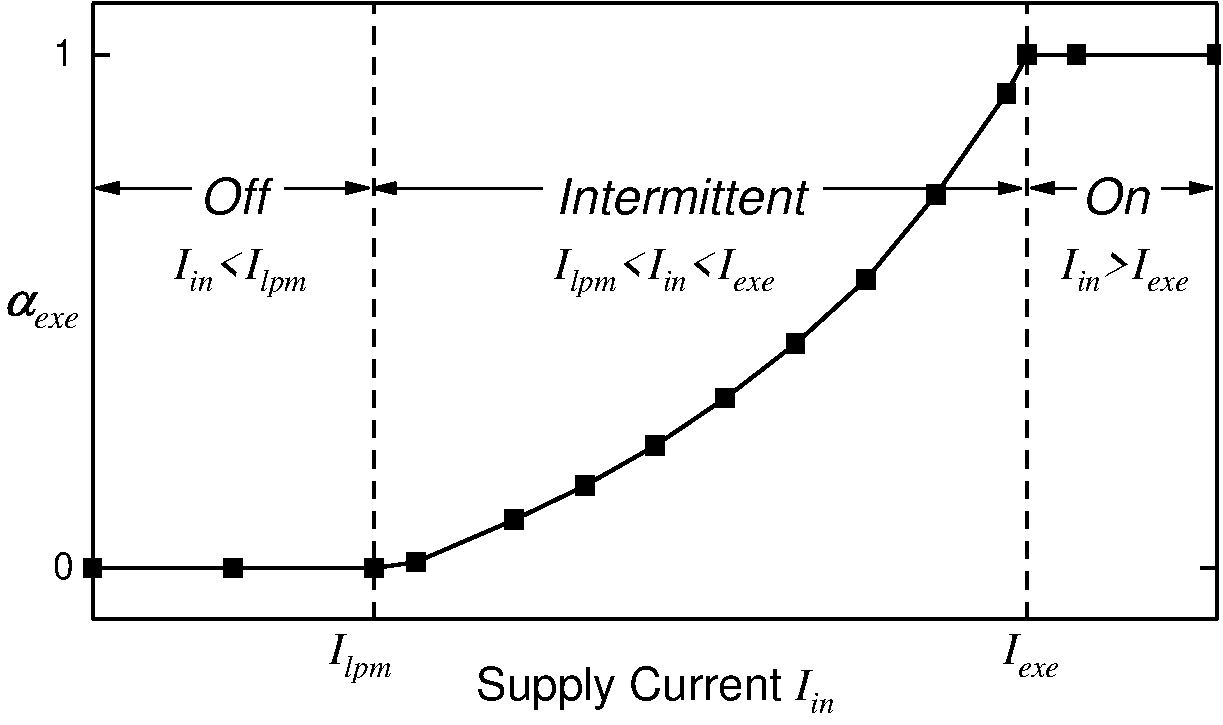
\includegraphics[width=0.8\columnwidth]{ch3_sizingeffect/figures/OperatingMode0Fig}
    \caption{Operating modes of reactive ICSs, and achieved forward progress against supply current.}
    \label{fig:operatingModes}
\end{figure}

\begin{itemize}
	\item \textit{Off} mode: When $\nmm{I}{in} < \nmm{I}{lpm}$, the system stays inactive. The supply voltage \nm{V}{cc} cannot rise above the restore threshold \nm{V}{r} to wake the system and start execution. The LPM current \nm{I}{lpm} includes the consumption of voltage monitoring circuits and system idle current.
	% Here, \nm{I}{lpm} is induced after \nm{V}{cc} goes above the minimum operating voltage $V_{off}$ where the system waits for \nm{V}{cc} to reach \nm{V}{r} (when $V_{off} < \nmm{V}{cc} < \nmm{V}{r}$). 

    \item \textit{On} mode: When $\nmm{I}{in} > \nmm{I}{exe}$, the system executes constantly as the supply voltage \nm{V}{cc} never drops below \nm{V}{s}. \nm{V}{cc} grows until \nm{I}{in} and \nm{I}{exe} are in equilibrium, which may result from \nm{I}{in} decreasing due to poor impedance matching, or \nm{I}{exe} increasing due to either greater current draw at higher voltage or dissipation through overvoltage protection circuits. 

	\item \textit{Intermittent} mode: When $\nmm{I}{lpm} < \nmm{I}{in} < \nmm{I}{exe}$, the system executes intermittently after $\nmm{V}{cc} > \nmm{V}{r}$ and before $\nmm{V}{cc} < \nmm{V}{s}$. \nm{V}{cc} can rise above \nm{V}{r} and the system starts execution. However, the stored energy is then consumed by the load as $\nmm{I}{in} < \nmm{I}{exe}$, causing \nm{V}{cc} to eventually drop below the save threshold \nm{V}{s}, where the system saves its state and enters LPM. The system stays in LPM until \nm{V}{cc} rises to \nm{V}{r} again and then resumes execution. 
	% In this mode, \nm{V}{cc} oscillates approximately between \nm{V}{r} and \nm{V}{s}, 'switching' on and off the execution. 
    In general, a higher \nm{I}{in} leads to more forward progress in this mode, but the exact relationship between \nm{I}{in} and forward progress requires further analysis.
    
	% The excess power either dissipates through circuits or overcharges \nm{V}{cc}. An overcharged \nm{V}{cc} may affect harvesting efficiency due to poor impedance matching and reduce \nm{I}{harv}, such that current input and consumption are in equilibrium. 
	% In this model case, charging \nm{V}{cc} above the maximum power point of the PV cell reduces $I_{harvest}$, and \nm{V}{cc} is stable when $I_{harvest} = \nmm{I}{exe} + \nmm{I}{leak}$. 
\end{itemize}

\subsection{Formulating Forward Progress} \label{subsec:formulation}

Next, we derive formulations to calculate \nm{\alpha}{exe} from \nm{I}{in} and energy storage capacitance \N{C}. We then explore the effect of capacitor leakage on maximum forward progress. 

In the \textit{On} and \textit{Off} modes, the normalised forward progress is trivial to find (simply 1 and 0 respectively). In the \textit{Intermittent} mode,  as shown in \fref{fig:operatingCycle}, the system goes through four intervals in turn, i.e. charging, restoring, executing, and saving, with current consumption of \nm{I}{lpm}, \nm{I}{r}, \nm{I}{exe}, and \nm{I}{s} in each interval respectively. The normalised forward progress, i.e. effective execution time ratio, is indicated as $\nmm{T}{exe} / \nmm{T}{cycle}$, where \nm{T}{exe} is the time spent on effective execution in one operating cycle and \nm{T}{cycle} is the period of operating cycles. Hence, the forward progress given all supply levels is expressed as:
\begin{equation}
    \nmm{\alpha}{exe} = \left\{
    \begin{aligned}
        & 0 & , & \quad \textit{Off} \, (\nmm{I}{in} < \nmm{I}{lpm}) \\
        & \frac{\nmm{T}{exe}}{\nmm{T}{cycle}} & , & \quad \textit{Intermittent} \, (\nmm{I}{lpm} < \nmm{I}{in} < \nmm{I}{exe}) \\
        & 1 & , & \quad \textit{On} \, (\nmm{I}{in} > \nmm{I}{exe})
    \end{aligned}
    \right.
    \label{eq:feff}
\end{equation}

\begin{figure}[!t]
    \centering
    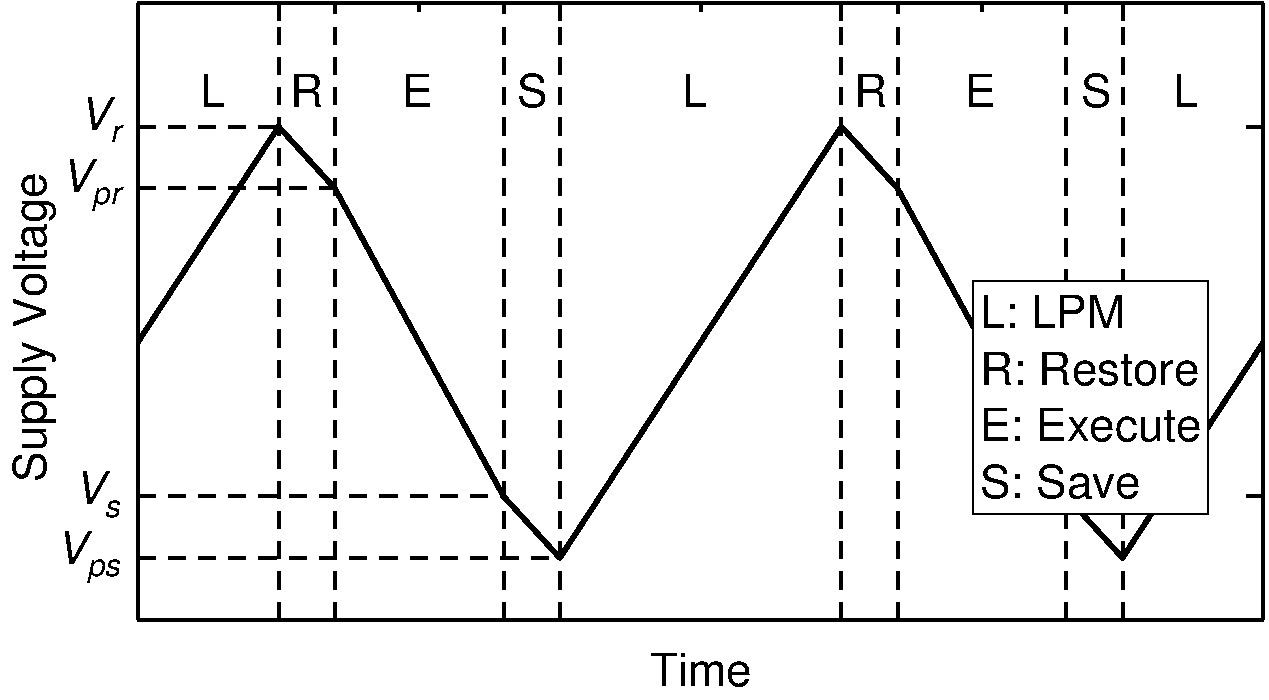
\includegraphics[width=0.8\columnwidth]{ch3_sizingeffect/figures/CRESdemoFig}
    \caption{Operating cycles in the \textit{Intermittent} mode. }
    \label{fig:operatingCycle}
\end{figure}

In the following analysis, we focus on deriving $\nmm{T}{exe} / \nmm{T}{cycle}$ in the \textit{Intermittent} mode. Let \nm{V}{pr} (post-restore) and \nm{V}{ps} (post-save) denote the voltage after restoring and saving operations. \nm{V}{pr} and \nm{V}{ps} can be calculated as:
\begin{equation}
    \nmm{V}{pr} = \nmm{V}{r} + \frac{\nmm{T}{r} (\nmm{I}{in} - \nmm{I}{r})}{C}
    \label{eq:vpr}
\end{equation}
\begin{equation}
    \nmm{V}{ps} = \nmm{V}{s} + \frac{\nmm{T}{s} (\nmm{I}{in} - \nmm{I}{s})}{C}
    \label{eq:vps}
\end{equation}
With \eref{eq:vpr}, the time spent on effective execution \nm{T}{exe} in one operating cycle can be expressed as:
\begin{equation}
    \begin{aligned}
        \nmm{T}{exe} & = \frac{C(\nmm{V}{pr} - \nmm{V}{s})}{\nmm{I}{exe} - \nmm{I}{in}} \\
        & = \frac{C(\nmm{V}{r} - \nmm{V}{s}) + \nmm{T}{r} (\nmm{I}{in} - \nmm{I}{r})} {\nmm{I}{exe} - \nmm{I}{in}}
    \end{aligned}
    \label{eq:texe}
\end{equation}
Analogously, with \eref{eq:vps}, the charging interval can be described as:
\begin{equation}
    \begin{aligned}
        T_{charge} & = \frac{C(\nmm{V}{r} - \nmm{V}{ps})}{\nmm{I}{in} - \nmm{I}{lpm}} \\
        & = \frac{C(\nmm{V}{r} - \nmm{V}{s}) - \nmm{T}{s} (\nmm{I}{in} - \nmm{I}{s})} {\nmm{I}{in} - \nmm{I}{lpm}}
    \end{aligned}
    \label{eq:tcharge}
\end{equation}
With \eref{eq:texe} and \eref{eq:tcharge}, the period of an operating cycle is:
\begin{equation}
    \begin{aligned}
        \nmm{T}{cycle} & = \quad T_{charge} + \nmm{T}{r} + \nmm{T}{exe} + \nmm{T}{s} \\
        & = \quad \frac{C (\nmm{V}{r} - \nmm{V}{s}) + \nmm{T}{s} (\nmm{I}{s} - \nmm{I}{lpm})}{\nmm{I}{in} - \nmm{I}{lpm}} + \frac{C (\nmm{V}{r} - \nmm{V}{s}) + \nmm{T}{r} (\nmm{I}{exe} - \nmm{I}{r})}{\nmm{I}{exe} - \nmm{I}{in}}
    \end{aligned}
    \label{eq:tperiod}
\end{equation}

Finally, combining \eref{eq:vpr} to \eref{eq:tperiod}, we obtain normalised forward progress \nm{\alpha}{exe} in the \textit{Intermittent} mode ($\nmm{I}{lpm} < \nmm{I}{in} < \nmm{I}{exe}$) as:
\begin{equation}
    \begin{aligned}
        \nmm{\alpha}{exe} &= \frac{\nmm{T}{exe}}{\nmm{T}{cycle}} \\
        &= [\frac{C (\nmm{V}{r} - \nmm{V}{s}) + \nmm{T}{r} (\nmm{I}{in} - \nmm{I}{r})} {\nmm{I}{exe} - \nmm{I}{in}}] / \\
        & [\frac{C (\nmm{V}{r} - \nmm{V}{s}) + \nmm{T}{s} (\nmm{I}{s} - \nmm{I}{lpm})}{\nmm{I}{in} - \nmm{I}{lpm}} + \frac{C (\nmm{V}{r} - \nmm{V}{s}) + \nmm{T}{r} (\nmm{I}{exe} - \nmm{I}{r})}{\nmm{I}{exe} - \nmm{I}{in}}] \\
    \end{aligned}
    \label{eq:texepercent}
\end{equation}
In the numerator \nm{T}{exe}, $C(\nmm{V}{r} - \nmm{V}{s})$ represents the amount of charge in the capacitor available for restoring and executing. $\nmm{T}{r} (\nmm{I}{in} - \nmm{I}{r})$ represents the charge used by a restore operation. $\nmm{I}{exe} - \nmm{I}{in}$ is the rate of charge consumption from the energy storage during execution.

% \footnote{Calculation breakdowns of differential analysis is attached in Appendix.}
% Higher \nm{\alpha}{exe} leads to more time spent on forward progress. 

% As $d\nmm{\alpha}{exe} / d\nmm{I}{in}$ is positive, higher harvested current \nm{I}{harv} leads to more forward progress. 
To explore the effect of energy storage on forward progress, we need to analyse $d\nmm{\alpha}{exe} / dC$. Here, if we assume that \nm{I}{leak} remains constant, \nm{\alpha}{exe} keeps increasing and approaches $(\nmm{I}{in} - \nmm{I}{lpm}) / (\nmm{I}{exe} - \nmm{I}{lpm})$ when energy storage capacitance \N{C} increases. Defining $(\nmm{I}{in} - \nmm{I}{lpm}) / (\nmm{I}{exe} - \nmm{I}{lpm})$ as \nm{\alpha}{exe\_ideal}, $\nmm{\alpha}{exe} = \nmm{\alpha}{exe\_ideal}$ is an ideal case, where restore and save overheads are absent.

In an electrolytic capacitor, however, \nm{I}{leak} typically increases with \N{C} with the following relationship~\cite{avxleakage}:
\begin{equation}
    \nmm{I}{leak} = kC\nmm{V}{cc}
    \label{eq:ileak}
\end{equation}
where $k$ is a constant normally in a range of \SIrange{0.01}{0.03}{\ampere\per\farad\per\volt}. Combining \eref{eq:ileak} with \eref{eq:in}, $d\nmm{I}{in} / dC$ is $-k\nmm{V}{cc}$, meaning \nm{I}{in} decreases linearly as \N{C} increases. Thus, when \N{C} increases, \nm{\alpha}{exe} keeps approaching \nm{\alpha}{exe\_ideal} while \nm{\alpha}{exe\_ideal} decreases. Hence, we believe that there is a capacitance value that leads to the maximum \nm{\alpha}{exe} considering \nm{I}{leak} increases with \N{C}.
% \cite{alcapacitor}
% Also, the time overhead of state saving and restoring operations $T_{RS\%}$ can be calculated as:
% \begin{equation}
%   T_{RS\%} = \frac{\nmm{T}{r} + \nmm{T}{s}}{\nmm{T}{exe} + \nmm{T}{r} + \nmm{T}{s}}
% \end{equation}


% In Equation~(\ref{eq:feff}), we get the relationship between forward progress and the sizes of energy harvester and energy storage. 
                       % Old Sec IV
\section{Experimental Evaluation} \label{sec:experiment}

\subsection{Benchmark and Comparisons}

Benchmark: 

\begin{itemize}
    \item AES encryption. Default 128-bit 4KB.
    \item RF transmission. Default 32B payload, 2Mbps.
    \item DMA
    \item Sensor? (possible)
\end{itemize}

Comparisons:

DEBS, Samoyed (later), Plain C (for evaluating overheads)

We may temporarily overlook Samoyed as its implementation is a bit more complex and its threshold setting is unclear. 
Samoyed scales down the atomic task if it fails to complete (but never scale back). 
It uses an "energy profiler" in previous work to test the whether the smallest scale of all peripheral tasks and randomized inputs can successfully complete. 
They suggested it is appropriate to set an energy capacity that can run the smallest scale of an operation for hundreds of times in one active cycle. 
Hence, it does not look for a threshold for a task with a specific configuration, but instead its aim is to minimize the chance of non-termination in practice by giving a high margin.

\subsection{Profiling Accuracy}

Question: How does our profiling approach perform in terms of accuracy?

Accuracy compared to manual measurement.

Figure shows:
\begin{itemize}
    \item Profiling results (average of 10)
    \item Each profiling reading (range)
    \item Dynamic threshold (Perhaps add horizontal lines as configurable thresholds in figures)
    \item Manually profiled voltage drop (average of 5 readings)
    \item Comparison against
\end{itemize}

\begin{figure}[t]
    \centering
    \begin{tikzpicture}
    \begin{groupplot}[
        group style={group size=3 by 1,horizontal sep=5pt},
        width=0.4\columnwidth, height=5cm,
        xmin=-13,xmax=13,
        ymin=0,ymax=110,
        xtick distance=5,
        ytick distance=20,
        xticklabel pos=bottom,
        every tick label/.append style={font=\small},
        minor x tick num=0,
        area style,
        xlabel={Error (\SI{}{\milli\volt})},
        xlabel style={yshift=3pt,},
        title style={at={(0.5,0)},anchor=north,yshift=-1.5cm},
        ]

        \nextgroupplot [title={(a) DMA},yticklabel={\pgfmathprintnumber\tick\%}]
        \addplot 
            plot [ybar interval,mark=no,black,fill=Set1-B,]
            table [x=v_error,y=repa_dma,col sep=comma] {ch5_optic/figures/profiling_accuracy/profiling_accuracy.csv};
        \node (n1) at (axis cs:0,100) {};
        \node (n2) at (axis cs:0,0) {};
        \draw [color=Set1-A,ultra thick,dashed] (n2) -- (n1);
        \node [anchor=north, font=\footnotesize, color=Set1-A] at (axis cs:0,108) {$\Delta V_{\text{task}}$=\SI{107}{\milli\volt}};

        \nextgroupplot [title={(b) AES},yticklabel=\empty]
        \addplot 
            plot [ybar interval,mark=no,black,fill=Set1-B,]
            table [x=v_error,y=repa_aes,col sep=comma] {ch5_optic/figures/profiling_accuracy/profiling_accuracy.csv};
        \node (n1) at (axis cs:0,100) {};
        \node (n2) at (axis cs:0,0) {};
        \draw [color=Set1-A,ultra thick,dashed] (n2) -- (n1);
        \node [anchor=north, font=\footnotesize, color=Set1-A] at (axis cs:0,108) {$\Delta V_{\text{task}}$=\SI{583}{\milli\volt}};

        \nextgroupplot [title={(c) RF},yticklabel=\empty]
        \addplot 
            plot [ybar interval,mark=no,black,fill=Set1-B,]
            table [x=v_error,y=repa_radio,col sep=comma] {ch5_optic/figures/profiling_accuracy/profiling_accuracy.csv};
        \node (n1) at (axis cs:0,100) {};
        \node (n2) at (axis cs:0,0) {};
        \draw [color=Set1-A,ultra thick,dashed] (n2) -- (n1);
        \node [anchor=north, font=\footnotesize, color=Set1-A] at (axis cs:0,108) {$\Delta V_{\text{task}}$=\SI{720}{\milli\volt}};
    \end{groupplot}
    \end{tikzpicture}
    \caption{\nn{} Profiling accuracy. }
    \label{fig:profiling_accuracy}
\end{figure} 

% Old figure
% \begin{figure*}[t]
%     \centering
%     \begin{tikzpicture}
%     \begin{groupplot}[
%         group style={group size=3 by 2, vertical sep=43pt},
%         width=0.7\columnwidth, height=3.7cm,
%         xmin=-15,xmax=15,
%         ymin=0,ymax=100,
%         xtick distance=5,
%         % xtick pos=top,
%         xticklabel pos=bottom,
%         yticklabel={\pgfmathprintnumber\tick\%},
%         every tick label/.append style={font=\small},
%         minor x tick num=0,
%         area style,
%         xlabel={Error (\SI{}{\milli\volt})},
%         xlabel style={yshift=3pt,},
%         title style={yshift=-7pt,},
%         ]

%         \nextgroupplot [title={(a) REPA, DMA Transfer}]
%         \addplot 
%             plot [ybar interval,mark=no,black,fill=Set1-B,]
%             table [x=v_error,y=repa_dma,col sep=comma] {figures/profiling_accuracy/profiling_accuracy.csv};
%         \node [anchor=north, font=\footnotesize, color=Set1-A] (n1) at (axis cs:0,100) {\SI{107}{\milli\volt}};
%         \node (n2) at (axis cs:0,0) {};
%         \draw [color=Set1-A,thick,dashed] (n2) -- (n1);

%         \nextgroupplot [title={(b) REPA, AES Encryption}]
%         \addplot 
%             plot [ybar interval,mark=no,black,fill=Set1-B,]
%             table [x=v_error,y=repa_aes,col sep=comma] {figures/profiling_accuracy/profiling_accuracy.csv};
%         \node [anchor=north, font=\footnotesize, color=Set1-A] (n1) at (axis cs:0,100) {\SI{583}{\milli\volt}};
%         \node (n2) at (axis cs:0,0) {};
%         \draw [color=Set1-A,thick,dashed] (n2) -- (n1);

%         \nextgroupplot [title={(c) REPA, Radio Transmission}]
%         \addplot 
%             plot [ybar interval,mark=no,black,fill=Set1-B,]
%             table [x=v_error,y=repa_radio,col sep=comma] {figures/profiling_accuracy/profiling_accuracy.csv};
%         \node [anchor=north, font=\footnotesize, color=Set1-A] (n1) at (axis cs:0,100) {\SI{720}{\milli\volt}};
%         \node (n2) at (axis cs:0,0) {};
%         \draw [color=Set1-A,thick,dashed] (n2) -- (n1);

%         \nextgroupplot [title={(d) Naive, DMA Transfer}]
%         \addplot 
%             plot [ybar interval,mark=no,black,fill=Set1-B,]
%             table [x=v_error,y=naive_dma,col sep=comma] {figures/profiling_accuracy/profiling_accuracy.csv};
%         \node [anchor=north, font=\footnotesize, color=Set1-A] (n1) at (axis cs:0,100) {\SI{107}{\milli\volt}};
%         \node (n2) at (axis cs:0,0) {};
%         \draw [color=Set1-A,thick,dashed] (n2) -- (n1);

%         \nextgroupplot [title={(e) Naive, AES Encryption}]
%         \addplot 
%             plot [ybar interval,mark=no,black,fill=Set1-B,]
%             table [x=v_error,y=naive_aes,col sep=comma] {figures/profiling_accuracy/profiling_accuracy.csv};
%         \node [anchor=north, font=\footnotesize, color=Set1-A] (n1) at (axis cs:0,100) {\SI{583}{\milli\volt}};
%         \node (n2) at (axis cs:0,0) {};
%         \draw [color=Set1-A,thick,dashed] (n2) -- (n1);

%         \nextgroupplot [title={(f) Naive, Radio Transmission}]
%         \addplot 
%             plot [ybar interval,mark=no,black,fill=Set1-B,]
%             table [x=v_error,y=naive_radio,col sep=comma] {figures/profiling_accuracy/profiling_accuracy.csv};
%         \node [anchor=north, font=\footnotesize, color=Set1-A] (n1) at (axis cs:0,100) {\SI{720}{\milli\volt}};
%         \node (n2) at (axis cs:0,0) {};
%         \draw [color=Set1-A,thick,dashed] (n2) -- (n1);
        
%     \end{groupplot}


%     \end{tikzpicture}
%     \caption{Profiling accuracy. }
%     \label{fig:profiling_accuracy}
% \end{figure*} 


% \begin{figure}[!t]
    \centering
    \begin{tikzpicture}
    \begin{axis}[
        width=\columnwidth,
        height=5cm,
        ymin=0,ymax=65,
        xmin=2,xmax=12,
        xlabel={System Capacitance (\SI{}{\micro\farad})},
        ylabel={Completion rate (Hz)},
        % legend style={at={(0.05,0.95)},
            % anchor=north west,legend columns=1},
        % scaled y ticks=manual:{}{%
        %     \pgfmathparse{#1/13.8}%
        % },
        legend style={at={(0.5,1.05)},
            anchor=south,legend columns=2,
            /tikz/every even column/.append style={column sep=0.1cm}},
        ]
        \addplot
            plot [Set1-B,mark=*]
            table [x=capacitance, y=opta_perf,col sep=comma] {figures/capacitance/relia_cap_dma.csv};
        \addplot
            plot [Set1-B,mark=square*]
            table [x=capacitance, y=opta_perf,col sep=comma] {figures/capacitance/relia_cap_aes.csv};
        \addplot
            plot [Set1-A,mark=*,dashed]
            table [x=capacitance, y=debs_perf,col sep=comma] {figures/capacitance/relia_cap_dma.csv};
        \addplot
            plot [Set1-A,mark=square*,dashed]
            table [x=capacitance, y=debs_perf,col sep=comma] {figures/capacitance/relia_cap_aes.csv};
        \legend{REPA DMA, REPA AES, DEBS DMA, DEBS AES}
    \end{axis}
    \end{tikzpicture}
    \caption{Completion rate on variable capacitance.}
    \label{fig:reliability_capacitance_performance}
\end{figure}

% \begin{figure}[!t]
    \centering
    \begin{tikzpicture}
    \begin{axis}[
        width=\columnwidth,
        height=5cm,
        ymin=1.8,ymax=4,
        xmin=2,xmax=12,
        xlabel={System Capacitance (\SI{}{\micro\farad})},
        ylabel={Voltage thresholds (V)},
        legend style={at={(0.5,1.05)},
            anchor=south,legend columns=2,
            /tikz/every even column/.append style={column sep=0.1cm}},
        ]
        \addplot
            plot [Set1-B,mark=square*]
            table [x=capacitance, y=opta_thresh,col sep=comma] {figures/capacitance/relia_cap_aes.csv};
        \addplot
            plot [Set1-B,mark=*]
            table [x=capacitance, y=opta_thresh,col sep=comma] {figures/capacitance/relia_cap_dma.csv};
        \addplot
            plot [Set1-A,mark=square*,dashed]
            table [x=capacitance, y=debs_thresh,col sep=comma] {figures/capacitance/relia_cap_aes.csv};
        \addplot
            plot [Set1-A,mark=*,dashed]
            table [x=capacitance, y=debs_thresh,col sep=comma] {figures/capacitance/relia_cap_dma.csv};
        \legend{REPA DMA, REPA AES, DEBS DMA, DEBS AES}
    \end{axis}
    \end{tikzpicture}
    \caption{Thresholds on variable capacitance.}
    \label{fig:reliability_capacitance_thresholds}
\end{figure}



% \begin{figure*}[t]
%     \centering
%     \begin{tikzpicture}
%     \begin{groupplot}[
%         group style={group size=1 by 2,vertical sep=2pt},
%         width=0.5\columnwidth,
%         xmin=0,xmax=80,
%         every tick label/.append style={font=\small},
%         minor x tick num=0,
%         ]

%         % (a) upper
%         \nextgroupplot[
%             const plot,
%             height=4cm,
%             ymin=-0.2,ymax=1.2,
%             ytick distance=1,
%             xticklabel=\empty,
%             yticklabels={,Fail,Done},
%             legend style={
%                 anchor=west,
%                 at={(0.02,0.5)},
%                 font=\footnotesize,
%                 legend columns=2,
%             },
%             ]
%         \addplot 
%             plot [Set1-B,mark=o]
%             table [x=cap_reduction,y=opta_perf,col sep=comma] {ch5_optic/figures/capacitance/cap_test_dma.csv};
%         \addplot 
%             plot [Set1-A,mark=square]
%             table [x=cap_reduction,y=debs_perf,col sep=comma] {ch5_optic/figures/capacitance/cap_test_dma.csv};
%         \legend{\nn{},\debs{}}

%         % (b) upper
%         \nextgroupplot[
%             const plot,
%             height=4cm,
%             ymin=-0.2,ymax=1.2,
%             ytick distance=1,
%             xticklabel=\empty,
%             yticklabels={,Fail,Done},
%             legend style={
%                 anchor=west,
%                 at={(0,0.5)},
%                 font=\footnotesize,
%                 legend columns=2,
%             },
%             ]
%         \addplot 
%             plot [Set1-B,mark=o]
%             table [x=cap_reduction,y=opta_perf,col sep=comma] {ch5_optic/figures/capacitance/cap_test_aes.csv};
%         \addplot 
%             plot [Set1-A,mark=square]
%             table [x=cap_reduction,y=debs_perf,col sep=comma] {ch5_optic/figures/capacitance/cap_test_aes.csv};
%         % \legend{\nn{},\debs{}}

%         % (a) lower
%         \nextgroupplot[
%             height=6cm,
%             title={(a) DMA},
%             title style={at={(0.5,0)},anchor=north,yshift=-30pt,},
%             ymin=1.7,ymax=2.5,
%             xlabel={Capacitance Reduction},
%             ylabel={Start \& End Voltage (V)},
%             ytick distance=0.2,
%             xlabel style={yshift=3pt,},
%             xticklabel={\pgfmathprintnumber\tick\%},
%             legend style={
%                 anchor=north west,
%                 at={(0.02,0.98)},
%                 font=\footnotesize,
%                 legend columns=2,
%             },
%             ]
%         \addplot 
%             plot [Set1-B,mark=*]
%             table [x=cap_reduction,y=opta_v_start,col sep=comma] {ch5_optic/figures/capacitance/cap_test_dma.csv};
%         \addplot 
%             plot [Set1-B,mark=o]
%             table [x=cap_reduction,y=opta_v_end,col sep=comma] {ch5_optic/figures/capacitance/cap_test_dma.csv};
%         \addplot 
%             plot [Set1-A,mark=square*]
%             table [x=cap_reduction,y=debs_v_start,col sep=comma] {ch5_optic/figures/capacitance/cap_test_dma.csv};
%         \addplot 
%             plot [Set1-A,mark=square]
%             table [x=cap_reduction,y=debs_v_end,col sep=comma] {ch5_optic/figures/capacitance/cap_test_dma.csv};
%         \draw [thick,dashed] (axis cs:0,2) -- (axis cs:80,2);
%         \node [anchor=north east,font=\small] at (axis cs:80,2) {Target $V_{\text{end}}$};
%         \draw [thick,dashed] (axis cs:0,1.8) -- (axis cs:80,1.8);
%         \node [anchor=north east,font=\small] at (axis cs:80,1.8) {Fail};
%         \legend{\ ,\nn{} $V_{\text{start}}\ V_{\text{end}}$,\ ,\debs{} $V_{\text{start}}\ V_{\text{end}}$}

%         % (b) lower
%         \nextgroupplot[
%             height=6cm,
%             title={(b) AES},
%             title style={at={(0.5,0)},anchor=north,yshift=-30pt,},
%             ymin=1.55,ymax=3.7,
%             xlabel={Capacitance Reduction},
%             ytick distance=0.5,
%             extra y ticks={1.8},
%             xlabel style={yshift=3pt,},
%             xticklabel={\pgfmathprintnumber\tick\%},
%             legend style={
%                 anchor=north west,
%                 at={(0,1)},
%                 font=\footnotesize,
%                 legend columns=2,
%             },
%             ]
%         \addplot 
%             plot [Set1-B,mark=*]
%             table [x=cap_reduction,y=opta_v_start,col sep=comma] {ch5_optic/figures/capacitance/cap_test_aes.csv};
%         \addplot 
%             plot [Set1-B,mark=o]
%             table [x=cap_reduction,y=opta_v_end,col sep=comma] {ch5_optic/figures/capacitance/cap_test_aes.csv};
%         \addplot 
%             plot [Set1-A,mark=square*]
%             table [x=cap_reduction,y=debs_v_start,col sep=comma] {ch5_optic/figures/capacitance/cap_test_aes.csv};
%         \addplot 
%             plot [Set1-A,mark=square]
%             table [x=cap_reduction,y=debs_v_end,col sep=comma] {ch5_optic/figures/capacitance/cap_test_aes.csv};
%         \draw [thick,dashed] (axis cs:0,2) -- (axis cs:80,2);
%         \node [anchor=south east,font=\small] at (axis cs:80,2) {Target $V_{\text{end}}$};
%         \draw [thick,dashed] (axis cs:0,1.8) -- (axis cs:80,1.8);
%         \node [anchor=north east,font=\small] at (axis cs:80,1.8) {Fail};
%         % \legend{\ ,\nn{} $V_{\text{start}}\ V_{\text{end}}$,\ ,\debs{} $V_{\text{start}}\ V_{\text{end}}$}

%         % (c) upper
%         \nextgroupplot[
%             const plot,
%             height=4cm,
%             ymin=-0.2,ymax=1.2,
%             ytick distance=1,
%             xticklabel=\empty,
%             yticklabels={,Fail,Done},
%             legend style={
%                 anchor=west,
%                 at={(0,0.5)},
%                 font=\footnotesize,
%                 legend columns=2,
%             },
%             ]
%         \addplot 
%             plot [Set1-B,mark=o]
%             table [x=cap_reduction,y=opta_perf,col sep=comma] {ch5_optic/figures/capacitance/cap_test_radio.csv};
%         \addplot 
%             plot [Set1-A,mark=square]
%             table [x=cap_reduction,y=debs_perf,col sep=comma] {ch5_optic/figures/capacitance/cap_test_radio.csv};
%         % \legend{\nn{},\debs{}}
        
%         % (c) lower
%         \nextgroupplot[
%             height=6cm,
%             title={(c) RF},
%             title style={at={(0.5,0)},anchor=north,yshift=-30pt,},
%             ymin=1.72,ymax=3.3,
%             xlabel={Capacitance Reduction},
%             ylabel={Start \& End Voltage (V)},
%             ytick distance=0.4,
%             extra y ticks={1.9},
%             xlabel style={yshift=3pt,},
%             xticklabel={\pgfmathprintnumber\tick\%},
%             legend style={
%                 anchor=north west,
%                 at={(0,1)},
%                 font=\footnotesize,
%                 legend columns=2,
%             },
%             ]
%         \addplot 
%             plot [Set1-B,mark=*]
%             table [x=cap_reduction,y=opta_v_start,col sep=comma] {ch5_optic/figures/capacitance/cap_test_radio.csv};
%         \addplot 
%             plot [Set1-B,mark=o]
%             table [x=cap_reduction,y=opta_v_end,col sep=comma] {ch5_optic/figures/capacitance/cap_test_radio.csv};
%         \addplot 
%             plot [Set1-A,mark=square*]
%             table [x=cap_reduction,y=debs_v_start,col sep=comma] {ch5_optic/figures/capacitance/cap_test_radio.csv};
%         \addplot 
%             plot [Set1-A,mark=square]
%             table [x=cap_reduction,y=debs_v_end,col sep=comma] {ch5_optic/figures/capacitance/cap_test_radio.csv};
%         \draw [thick,dashed] (axis cs:0,2) -- (axis cs:80,2);
%         \node [anchor=south east,font=\small] at (axis cs:80,2) {Target $V_{\text{end}}$};
%         \draw [thick,dashed] (axis cs:0,1.9) -- (axis cs:80,1.9);
%         \node [anchor=north east,font=\small] at (axis cs:80,1.9) {Fail};
%         % \legend{\ ,\nn{} $V_{\text{start}}\ V_{\text{end}}$,\ ,\debs{} $V_{\text{start}}\ V_{\text{end}}$}

%     \end{groupplot}
%     \end{tikzpicture}
%     \caption{Capacitance test. }
%     \label{fig:capacitance_test}
% \end{figure*}



\begin{figure*}[t]
    \centering
    \begin{tikzpicture}
    \begin{groupplot}[
        group style={group size=1 by 2,vertical sep=2pt},
        width=0.7\columnwidth,
        xmin=0,xmax=80,
        every tick label/.append style={font=\small},
        minor x tick num=0,
        ]

        % (a) upper
        \nextgroupplot[
            const plot,
            height=4cm,
            ymin=-0.2,ymax=1.2,
            ytick distance=1,
            xticklabel=\empty,
            yticklabels={,Fail,Done},
            legend style={
                anchor=west,
                at={(0.02,0.5)},
                font=\footnotesize,
                legend columns=2,
            },
            ]
        \addplot 
            plot [Set1-B,mark=o]
            table [x=cap_reduction,y=opta_perf,col sep=comma] {ch5_optic/figures/capacitance/cap_test_dma.csv};
        \addplot 
            plot [Set1-A,mark=square]
            table [x=cap_reduction,y=debs_perf,col sep=comma] {ch5_optic/figures/capacitance/cap_test_dma.csv};
        \legend{\nn{},\debs{}}

        % (a) lower
        \nextgroupplot[
            height=6cm,
            title={(a) DMA},
            title style={at={(0.5,0)},anchor=north,yshift=-30pt,},
            ymin=1.7,ymax=2.5,
            xlabel={Capacitance Reduction},
            ylabel={Start \& End Voltage (V)},
            ytick distance=0.2,
            xlabel style={yshift=3pt,},
            xticklabel={\pgfmathprintnumber\tick\%},
            legend style={
                anchor=north west,
                at={(0.02,0.98)},
                font=\footnotesize,
                legend columns=2,
            },
            ]
        \addplot 
            plot [Set1-B,mark=*]
            table [x=cap_reduction,y=opta_v_start,col sep=comma] {ch5_optic/figures/capacitance/cap_test_dma.csv};
        \addplot 
            plot [Set1-B,mark=o]
            table [x=cap_reduction,y=opta_v_end,col sep=comma] {ch5_optic/figures/capacitance/cap_test_dma.csv};
        \addplot 
            plot [Set1-A,mark=square*]
            table [x=cap_reduction,y=debs_v_start,col sep=comma] {ch5_optic/figures/capacitance/cap_test_dma.csv};
        \addplot 
            plot [Set1-A,mark=square]
            table [x=cap_reduction,y=debs_v_end,col sep=comma] {ch5_optic/figures/capacitance/cap_test_dma.csv};
        \draw [thick,dashed] (axis cs:0,2) -- (axis cs:80,2);
        \node [anchor=north east,font=\small] at (axis cs:80,2) {Target $V_{\text{end}}$};
        \draw [thick,dashed] (axis cs:0,1.8) -- (axis cs:80,1.8);
        \node [anchor=north east,font=\small] at (axis cs:80,1.8) {Fail};
        \legend{\ ,\nn{} $V_{\text{start}}\ V_{\text{end}}$,\ ,\debs{} $V_{\text{start}}\ V_{\text{end}}$}

    \end{groupplot}
\end{tikzpicture}
\caption{Capacitance test. }
\label{fig:capacitance_test_a}
\end{figure*}


\begin{figure*}[t]
    \centering
    \begin{tikzpicture}
    \begin{groupplot}[
        group style={group size=1 by 2,vertical sep=2pt},
        width=0.7\columnwidth,
        xmin=0,xmax=80,
        every tick label/.append style={font=\small},
        minor x tick num=0,
        ]

        % (b) upper
        \nextgroupplot[
            const plot,
            height=4cm,
            ymin=-0.2,ymax=1.2,
            ytick distance=1,
            xticklabel=\empty,
            yticklabels={,Fail,Done},
            legend style={
                anchor=west,
                at={(0,0.5)},
                font=\footnotesize,
                legend columns=2,
            },
            ]
        \addplot 
            plot [Set1-B,mark=o]
            table [x=cap_reduction,y=opta_perf,col sep=comma] {ch5_optic/figures/capacitance/cap_test_aes.csv};
        \addplot 
            plot [Set1-A,mark=square]
            table [x=cap_reduction,y=debs_perf,col sep=comma] {ch5_optic/figures/capacitance/cap_test_aes.csv};
        \legend{\nn{},\debs{}}

        % (b) lower
        \nextgroupplot[
            height=6cm,
            title={(b) AES},
            title style={at={(0.5,0)},anchor=north,yshift=-30pt,},
            ymin=1.55,ymax=3.7,
            xlabel={Capacitance Reduction},
            ytick distance=0.5,
            extra y ticks={1.8},
            xlabel style={yshift=3pt,},
            xticklabel={\pgfmathprintnumber\tick\%},
            legend style={
                anchor=north west,
                at={(0,1)},
                font=\footnotesize,
                legend columns=2,
            },
            ]
        \addplot 
            plot [Set1-B,mark=*]
            table [x=cap_reduction,y=opta_v_start,col sep=comma] {ch5_optic/figures/capacitance/cap_test_aes.csv};
        \addplot 
            plot [Set1-B,mark=o]
            table [x=cap_reduction,y=opta_v_end,col sep=comma] {ch5_optic/figures/capacitance/cap_test_aes.csv};
        \addplot 
            plot [Set1-A,mark=square*]
            table [x=cap_reduction,y=debs_v_start,col sep=comma] {ch5_optic/figures/capacitance/cap_test_aes.csv};
        \addplot 
            plot [Set1-A,mark=square]
            table [x=cap_reduction,y=debs_v_end,col sep=comma] {ch5_optic/figures/capacitance/cap_test_aes.csv};
        \draw [thick,dashed] (axis cs:0,2) -- (axis cs:80,2);
        \node [anchor=south east,font=\small] at (axis cs:80,2) {Target $V_{\text{end}}$};
        \draw [thick,dashed] (axis cs:0,1.8) -- (axis cs:80,1.8);
        \node [anchor=north east,font=\small] at (axis cs:80,1.8) {Fail};
        \legend{\ ,\nn{} $V_{\text{start}}\ V_{\text{end}}$,\ ,\debs{} $V_{\text{start}}\ V_{\text{end}}$}

    \end{groupplot}
\end{tikzpicture}
\caption{Capacitance test. }
\label{fig:capacitance_test_b}
\end{figure*}



\begin{figure*}[t]
    \centering
    \begin{tikzpicture}
    \begin{groupplot}[
        group style={group size=1 by 2,vertical sep=2pt},
        width=0.7\columnwidth,
        xmin=0,xmax=80,
        every tick label/.append style={font=\small},
        minor x tick num=0,
        ]

        % (c) upper
        \nextgroupplot[
            const plot,
            height=4cm,
            ymin=-0.2,ymax=1.2,
            ytick distance=1,
            xticklabel=\empty,
            yticklabels={,Fail,Done},
            legend style={
                anchor=west,
                at={(0,0.5)},
                font=\footnotesize,
                legend columns=2,
            },
            ]
        \addplot 
            plot [Set1-B,mark=o]
            table [x=cap_reduction,y=opta_perf,col sep=comma] {ch5_optic/figures/capacitance/cap_test_radio.csv};
        \addplot 
            plot [Set1-A,mark=square]
            table [x=cap_reduction,y=debs_perf,col sep=comma] {ch5_optic/figures/capacitance/cap_test_radio.csv};
        % \legend{\nn{},\debs{}}
        
        % (c) lower
        \nextgroupplot[
            height=6cm,
            title={(c) RF},
            title style={at={(0.5,0)},anchor=north,yshift=-30pt,},
            ymin=1.72,ymax=3.3,
            xlabel={Capacitance Reduction},
            ylabel={Start \& End Voltage (V)},
            ytick distance=0.4,
            extra y ticks={1.9},
            xlabel style={yshift=3pt,},
            xticklabel={\pgfmathprintnumber\tick\%},
            legend style={
                anchor=north west,
                at={(0,1)},
                font=\footnotesize,
                legend columns=2,
            },
            ]
        \addplot 
            plot [Set1-B,mark=*]
            table [x=cap_reduction,y=opta_v_start,col sep=comma] {ch5_optic/figures/capacitance/cap_test_radio.csv};
        \addplot 
            plot [Set1-B,mark=o]
            table [x=cap_reduction,y=opta_v_end,col sep=comma] {ch5_optic/figures/capacitance/cap_test_radio.csv};
        \addplot 
            plot [Set1-A,mark=square*]
            table [x=cap_reduction,y=debs_v_start,col sep=comma] {ch5_optic/figures/capacitance/cap_test_radio.csv};
        \addplot 
            plot [Set1-A,mark=square]
            table [x=cap_reduction,y=debs_v_end,col sep=comma] {ch5_optic/figures/capacitance/cap_test_radio.csv};
        \draw [thick,dashed] (axis cs:0,2) -- (axis cs:80,2);
        \node [anchor=south east,font=\small] at (axis cs:80,2) {Target $V_{\text{end}}$};
        \draw [thick,dashed] (axis cs:0,1.9) -- (axis cs:80,1.9);
        \node [anchor=north east,font=\small] at (axis cs:80,1.9) {Fail};
        % \legend{\ ,\nn{} $V_{\text{start}}\ V_{\text{end}}$,\ ,\debs{} $V_{\text{start}}\ V_{\text{end}}$}
    \end{groupplot}
\end{tikzpicture}
\caption{Capacitance test. }
\label{fig:capacitance_test_c}
\end{figure*}

\begin{figure}[t]
    \centering
    \begin{tikzpicture}
    \begin{axis}[
        width=0.7\columnwidth, height=6cm,
        ybar,
        ymin=0,
        ymax=1,
        enlarge x limits=0.5,
        legend style={at={(0.5,1.05)},
            anchor=south,legend columns=-1,
            /tikz/every even column/.append style={column sep=0.2cm}},
        legend image code/.code={
            \draw [#1] (0cm,-0.1cm) rectangle (0.2cm,0.25cm);},
        ylabel={Relative Completion Rate},
        symbolic x coords={AES,RF},
        xtick=data,
        tick align=inside,
        ]
    \pgfplotstableread[col sep=comma]{ch5_optic/figures/datasize/datasize.csv}{\mytable};
    % Samoyed
    \addplot
        plot [black,fill=Set1-A,postaction={pattern=north east lines}]
        table [x index=0,y expr=\thisrowno{3} / \thisrowno{1}] {\mytable};
    % DEBS
    \addplot
        plot [black,fill=Set1-B,postaction={pattern=dots}]
        table [x index=0,y expr=\thisrowno{2} / \thisrowno{1}] {\mytable};
    % OPTA
    \addplot
        plot [black,fill=Set1-C,postaction={pattern=north west lines}]
        table [x index=0,y expr=\thisrowno{1} / \thisrowno{1}] {\mytable};
    \legend{Samoyed, \debs{}, \nn{}}
    \end{axis}
    \end{tikzpicture}
    \caption{Relative Completion Rates of Samoyed, \debs{}, and \nn{} with variable data sizes and a PV supply. }
    \label{fig:datasize}
\end{figure} 



\subsection{Reliability with Dynamic Energy Consumption}

Question: Can it still make forward progress correctly with changes (as listed below) while other SoA approaches can't? 


New categories:

\begin{itemize}
    \item Changing once: new operations, device/components variability (including capacitor tolerance).
    \item Changing slowly: capacitor ageing, device ageing, temperature, long-term configuration.
    \item Changing frequently: Data size, configurations. 
\end{itemize}


Cases of changes and experiments:

\subsubsection{New devices / operations (once)}

- Show the voltage trace that illustrates how it profiles and adapts on new devices or new operations. 

\subsubsection{Variability in capacitance due to ageing / tolerance (slowly changing)}

- Profile the tasks for DEBS with the target end voltage at 1.8V (need explanation on this) and 30uF capacitance. 

- Build a capacitor bank with a better granularity. The potential testing range of capacitance should be 1.5-11.5uF, with 1uF capacitors per step. 

- Decrease the capacitance step by step. Record the capacitance where DEBS fails, the performance, the adaptive thresholds, and possibly a voltage trace that shows what happens. 

Note that the threshold settings in this experiment are different from the profiling results due to different system capacitance, operating voltage, allowing some switching overheads, and the comparator precision and resolution. 

\subsubsection{Variability in peripheral configurations (single threshold for a rarely/slightly-changing configuration, multiple thresholds for frequently-changing configurations)}

- Profile the tasks for DEBS with the target end voltage at 1.8V and a "default" configuration. 
    
- Presumably DEBS can only complete the tasks with configurations that consumes the same or less energy as it was profiled, while OPTA adapts the threshold. 

\subsubsection{Variability in the amount of data to process (fast changing, but perhaps could be an unsuitable test case for reliability as it should violate the API requirement to make it fail)}
    
- This would be similar to the capacitance test but with a less granularity needed.

\subsection{Efficiency}

Question: Does it run faster than other SoA approaches (make more progress under the same energy condition) under conditions that all approaches can make forward progress?

Comparisons: DEBS, Samoyed.

Test conditions:
    
- (1) A constant data size (2) Randomised data sizes (DEBS threshold configured for the largest data size)

- A few levels of input current

\subsection{Overheads}

- Current \& time overheads of profiling and adaptation (with a further breakdown according to sub-operations) compared to Plain C. 

Time is measured by GPIO signals, and current is calculated by measuring voltage droops. 

The energy/charge consumption can also be calculated. 

- Memory overhead. Check the section sizes of the compiled code. Compared it to a PlainC version and a Hibernus-like IC version.  

% \subsection{Correctness of computational results (test its intermittent computing functionality, might not be important)}

% Question: does it produce correct results from atomic functions across power failures?

% Compare the output of our approach with intermittent supply vs Plain C solution with continuous supply. Use a computational workload probably, as an atomic function should be guaranteed to finish. 


% \subsection{Case Study}

% Apply the proposed approach on an application that includes multiple atomic operations and the device runs with dynamic energy consumption due to operating conditions. 
                  % Old Sec VI
%%%%%%%%%%%%%%%%%%%%%%%%%%%%%%%%%%%%%%%%%%%%%%%%%%%%%%%%%%
%%% Section 4: Sizing Method
%%%%%%%%%%%%%%%%%%%%%%%%%%%%%%%%%%%%%%%%%%%%%%%%%%%%%%%%%%

\section{Energy Storage Sizing Approach} \label{section:approach}

As mentioned, previous designs of intermittent computing typically adopt a minimised energy storage so as to minimise device dimensions and interruption periods. 
However, such a minimised energy storage leads to frequent save and restore operations, and reduces forward progress.
An appropriate capacitor size instead may balance the three factors. 

We propose a sizing approach which recommends appropriate energy storage capacitance for an ICS, trading off forward progress against capacitor volume and interruption periods. 
We present a system model which accepts real long-term data on environmental energy conditions. 
The three inputs can be swept for design exploration, but we focus on energy storage in this paper. 
The model outputs forward progress, capacitor volume, and interruption periods (defined in Section~\ref{subsec:harvstor}). 
These are subsequently traded off in a cost function to obtain the appropriate energy storage capacitance. 
This process is summarised in \figurename{~\ref{fig:sizingapproach}} with details explained as follows. 

\begin{figure}[!t]
    \centering
    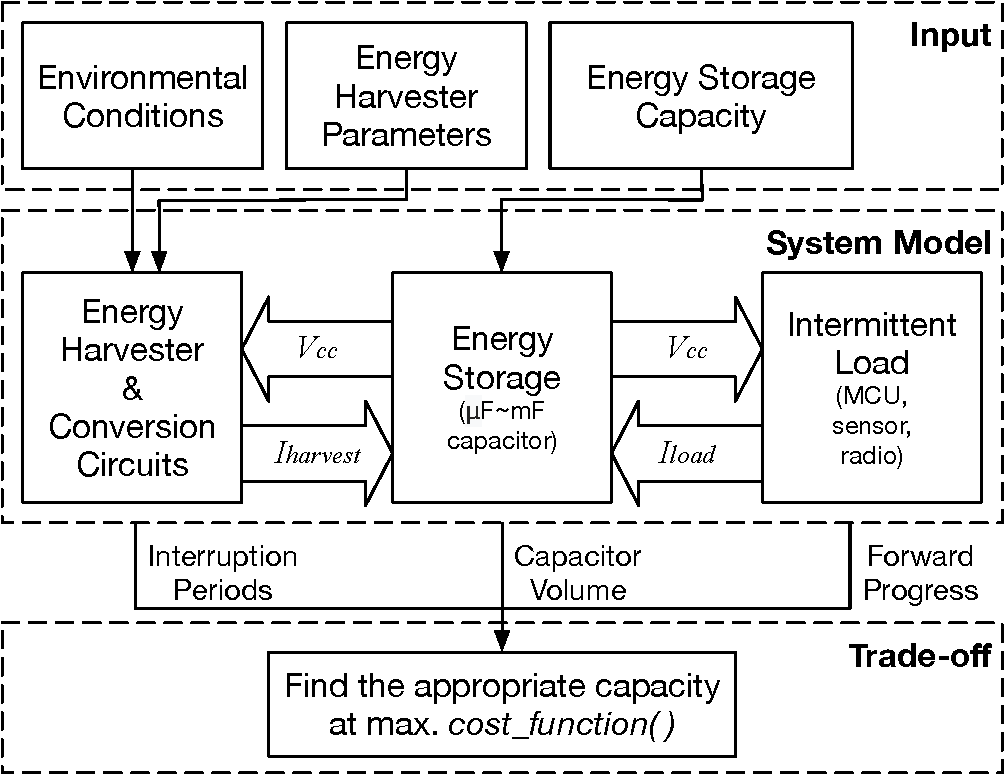
\includegraphics[width=0.8\columnwidth]{ch4_sizingapproach/figures/mdlfrw4}
    \caption{Structure of the proposed system model and sizing approach.}
    \label{fig:sizingapproach}
\end{figure}

    
\subsection{Input}
A time trace of representative environmental energy conditions in the intended deployment location is provided as an input, along with the energy harvester size. 
For design exploration, assuming the energy source is equally distributed in the deployed space, these can optionally be changed to explore variations and scales of harvested power. 
A pre-defined set of energy storage capacitance values are swept through. 

\subsection{System Model}

This contains three modules:
%Design exploration is enabled by changing parameters, for example energy storage and energy harvester sizes.
% As shown in \figurename{~\ref{fig:sizingapproach}}, the system model 
% We provide a system model as further explained in Section~\ref{subsec:systemmodel}. 
%, i.e. \textit{Energy Harvester and Conversion Circuits}, \textit{Energy Storage}, and \textit{Intermittent Load}. The current production $I_{harvest}$ and consumption $I_{load}$ are buffered in the energy storage, which then provides $V_{cc}$ for the load and the harvester output. Due to the variety in each module, they should be individually specified to represent the target platform according to the techniques implemented. 
% The three modules communicate by their voltage and current flows.
\begin{itemize}
    % [topsep=0pt]
    \item \textit{Energy Harvester and Conversion Circuits}: The energy harvester module transduces environmental energy into electricity. 
    % The harvested power is typically conditioned to provide a suitable voltage for charging the energy storage and supplying the load efficiently. 
    In ICSs, conversion circuits may simply be a diode to inhibit backflow of current.
    The energy harvester and conversion circuits can be modelled together as a module because they are usually coupled or integrated. 
    \item \textit{Energy Storage}: Energy storage in ICSs is usually in the form of a \SI{}{\micro\farad}-  to \SI{}{\milli\farad}-scale capacitor. It must be sufficient to complete the most energy-expensive atomic operation, and may be formed only of the decoupling capacitor(s). 
    %provides a minimum energy pulse, which should be set enough
    \item \textit{Intermittent Load}: Includes all the power consumers in an ICS, such as a microcontroller, sensors, and a radio. 
\end{itemize}

The outputs from the system model are the interruption periods, capacitor volume, and forward progress.
% As mentioned, ICS approaches can be classified as static and reactive approaches. These two types of approaches fundamentally differs in how the load consumes power and makes forward progress, and hence require different models for estimating forward progress. Owing to the computing advantage of reactive ICSs as explained in Section~\ref{section:review}, we focus on reactive ICSs for modelling and validation in this paper.
% The unit of energy source conditions should be consistent with the unit of the \textit{Energy Harvester and Conversion Circuits} in the ICS model. 
% Note that the size configuration of energy harvester configures actual dimensions, e.g. PV panel area, while the one of energy storage configures capacitance.
% The size configuration of energy harvester and energy storage can be altered to observe how the design metrics change. 

\subsection{Trade-off}
The appropriate capacitance is then found through a cost function. This may trade off forward progress against capacitor volume and interruption periods.
% The outputs are filtered and any results that fail to meet basic specifications for maximum interruption periods and minimum forward progress are discarded. 


% \begin{itemize}
%     \item [\textbf{S1-}] \textbf{Determine design specifications}: Derive specifications according to a target application, such as minimum forward progress, minimum energy storage capacitance, maximum capacitor dimensions, and maximum interruption periods under certain energy source conditions. 
%     \item [\textbf{S2-}] \textbf{Configure model}: Configure the model as explained in Section~\ref{sec:c2_model} according to the target platform and application, and collect energy source conditions of the environment where the device is deployed. 
%     \item [\textbf{S3-}] \textbf{Size Energy Harvester} With the configured model, run tests with the minimum capacitance, and find the energy harvester size to ensure the minimum forward progress under the given energy source conditions. 
%     \item [\textbf{S4-}] \textbf{Optimise capacitor size}: Generate the relationship between forward progress and capacitance. Evaluate the optimal capacitance by balancing the side effects of capacitor volume and interruption periods with forward progress in a cost function. A cost function is given in Equation~(\ref{eq:tradeoff}):
%     \begin{equation}
%         f = \frac{\alpha_{exe}}{k_1} - (\frac{v_{cap}}{k_2}) ^ {2} - (\frac{T_{recharge}}{k_3}) ^ {2} 
%         \label{eq:tradeoff}
%     \end{equation}
%     where $v_{cap}$ represents capacitor volume and $T_{recharge}$ represents interruption periods. $k_1$, $k_2$, and $k_3$ are linear scalers, which are empirically determined according to design specifications. The negative side effects are calculated in quadratic forms so as to punish high values more heavily. We only consider the above three factors in this paper to size energy storage, but other factors (e.g. dimensions of energy harvesters) can be included.
% \end{itemize}

% \subsection{System Model} \label{subsec:systemmodel}

% As shown in \figurename{~\ref{fig:sizingapproach}}, the system model contains three modules, i.e. \textit{Energy Harvester and Conversion Circuits}, \textit{Energy Storage}, and \textit{Intermittent Load}. The three modules communicate by their voltage and current flows. 
% Due to the variety in each module, the three module should be individually specified to represent the target platform according to the techniques implemented. 

% \subsubsection{Energy Harvester and Conversion Circuits} The energy harvester module transduces environmental energy into electrical power. The harvested power is typically conditioned to provide a suitable voltage for charging the energy storage and supplying the load efficiently. 
% However, in ICSs, such conversion circuits may be omitted, using only a diode to prevent current backflow. The energy harvester and conversion circuits can be modelled together as a module because they are usually coupled and integrated. 

% \subsubsection{Energy Storage} Energy storage in ICSs is usually in the form of a \SI{}{\micro\farad}-  to \SI{}{\milli\farad}-scale capacitor. The energy storage provides the minimum length of an execution period, which should be enough to complete the most energy-expensive atomic operation. 

% \subsubsection{Intermittent Load} The load module includes all the power consumers in an ICS, such as a microcontroller, sensors, and a radio. As mentioned, ICS approaches can be classified as \textit{static} and \textit{reactive}. These two types of approaches fundamentally differs in how the load consumes power and makes forward progress, and hence require different models for estimating forward progress. 

% This framework provides a guide to construct an EHIC system model that estimates forward progress of EHIC devices in real-world deployment. 
% based on an assumption that program progress is linear to effective execution time. 

% The model is driven by energy source conditions as a function of time. 

% This model outputs the time distribution of estimated forward progress over the test period of energy source input. 

% The size of energy harvester dominates the scale of power input. Given a constant source power, the harvested power typically increases with the size of energy harvester. For example, solar panel. 

% \footnote{Here, source power denotes the ambient energy source power exposed to energy harvester in a unit of the energy harvester model input. For example, if the energy harvester model is a photovoltaic (PV) cell model which takes irradiance as input, the source power should be defined in the unit of $W/m^2$. }

% Users should input a source power trace as a representation of the energy source conditions at the deployed site, and then alter the sizes of energy harvester and energy storage to explore the sizing effect on the design specifications. 

% For example, solar power from a solar panel is typically paired with a maximum power point tracking circuit to effectively extract solar power. The model should be configured for the specific energy harvester and the corresponding conversion circuits. 

% Static intermittent computing saves state at pre-installed points, and keeps executing until the supply fails, where the unsaved volatile progress is lost and the device has to re-execute from the last saved point. Reactive intermittent computing only saves state when the supply is about to fail (e.g. when the supply voltage is lower than a threshold), and then enters LPM (stop executing and enter a low-power mode). 
% However, to model intermittent computing is still a challenge due to lack of understanding and abstraction of its behaviours. 
% What is the difference of power consumption between these techniques? Power consumption: computing (CPU), memory R/W, peripherals (radio, ADC, sensor). While peripherals are more application-wise and currently we are not considering this, we focus more on memory R/W and CPU power. Memory R/W is related to both app and int techniques. Computing power, Memory R/W power. 

% \subsubsection{Model Outputs} 
% Define the outputs, e.g. forms, meanings. 
% Outputs come from which model in particular?

% Forward progress: a surface? 
% Dimensions: two (scattered) plots? 
% interruption periods: how do you define interruption periods, charging from where?                     % Old Sec III
\section{Design Exploration} 
\label{sec:design_exploration}

In this section, we study the variability in IPSs that can violate a predefined fixed threshold. 
We then investigate how existing approaches fail or become inefficient under this variability, and explore the potential of an adaptive thresholding scheme. 

\subsection{Variability in Intermittent Systems} 
\label{subsec:dynamic_energy_consumption}
 
Design-time profiling of workloads' energy consumption in the prior work can be potentially violated by the variability of IPSs.
To study and demonstrate the variability, we chose the built-in AES accelerator on the TI MSP430FR5994 microcontroller unit (MCU) as an example peripheral workload.  
The example AES function encrypts data in the cypher block chain mode, and can process up to 4KB data with a 128-, 192-, or 256-bit key length. 
In the following experiments, we measured $\Delta \symb{V}{task}$, \textit{the drop of supply voltage caused by an operation without any incoming energy meanwhile}, which directly determines the minimum voltage threshold that safely guarantees the completion of an atomic operation. 
We used Device 1 in Table~\ref{tab:device}, which has \SI{11.5}{\micro\farad} energy buffering capacitance, for the tests for variable data sizes and peripheral configurations, whereas in the device variability test we tested 3 devices.
We explored four factors that can possibly change $\Delta \symb{V}{task}$, which are variable data amounts, variable peripheral configurations, devices variability, and capacitor degradation and tolerance. 
Besides the above four, energy consumption can also change with other factors, such as temperature, clock frequency, and silicon ageing, but we have found them either insignificant or hard to validate on our experimental platform. 


% 22 uF extra capacitance, or 33 uF extra capacitance
% the MCU board has a 10 + 1.5 uF capacitance


\subsubsection{Variable Data Sizes}

A peripheral function can accept a runtime variable amount of data, such as a variable data size to encrypt or different lengths of packets for a radio to transmit. 
An example of this is plotted in Figure~\ref{fig:variable_datasize}, where the size of the square dots represent a \SI{5}{\milli\volt} precision error of the scope and the lines represent linear regression. 
We observed that $\Delta \symb{V}{task}$ has a linear relationship with the data size, with an offset energy consumption that accounts for the initialisation. 
%The dynamic range of $\Delta \symb{V}{task}$ is \SIrange{17}{194}{\milli\volt}.
In this case, the linearly scaled $\Delta \symb{V}{task}$ comes from linearly scaled run time. 

\begin{figure}[!t]
    \centering
    \begin{tikzpicture}
    \pgfplotsset{set layers}
    \begin{axis}[
        scale only axis,
        width=0.7\columnwidth,
        height=4cm,
        ymin=0,ymax=200,
        xmin=0,xmax=4,
        axis y line*=left,
        y axis line style={Set1-A},
        xlabel=Data Size to Encrypt (KiB),
        ylabel=$\Delta V_{\text{task}}$ (mV),
        legend style={at={(0.05,0.95)},
        anchor=north west,legend columns=1},
        ]
        \addplot
            plot [Set1-A,only marks,mark=square]
            table [x=data_size, y=voltage_drop,col sep=comma] {ch5_optic/figures/variable_data/variable_data.csv};
            \label{delta_V_task}
        \addplot
            plot [Set1-A]
            {44.31027668 * x + 16.926383399209485};
        % \legend{$\Delta V_{\text{task}}$}
    \end{axis}
    \begin{axis}[
        scale only axis,
        width=0.7\columnwidth,
        height=4cm,
        ymin=0,ymax=7,
        xmin=0,xmax=4,
        axis y line*=right,
        y axis line style={Set1-B},
        axis x line=none,
        ylabel=Run Time (ms),
        legend style={at={(0.95,0.05)},
        anchor=south east,legend columns=1},
        ]
        \addlegendimage{/pgfplots/refstyle=delta_V_task}\addlegendentry{$\Delta V_{\text{task}}$}
        \addplot
            plot [Set1-B,only marks,mark=o] 
            table [x=data_size, y=time,col sep=comma] {ch5_optic/figures/variable_data/variable_data.csv};
            \addlegendentry{Run Time}
        \addplot
            plot [Set1-B]
            {1.60436561 * x + 0.07670306324110676};
        % \legend{Run Time}
    \end{axis}
    \end{tikzpicture}
    \caption{$\Delta V_{\text{task}}$ varying linearly with the data size in AES 128-bit encryption.}
    \label{fig:variable_datasize}
\end{figure}


\subsubsection{Variability in Peripheral Configurations}

A peripheral can run with variable configurations at runtime, and demonstrate variable performance and energy consumption. 
For example, as shown in Table~\ref{tab:configurations}, an AES accelerator can encrypt data with 128-, 192-, or 256-bit keys. 
A longer key provides higher security, but also takes more time and energy to complete.
The dynamic range of configuration variability in this case can be a 26\% increase in $\Delta \symb{V}{task}$ and a 33\% increase in run time.
% Can refer to "A control flow" for the need of runtime configurations

\begin{table}
    \renewcommand{\arraystretch}{1.2}
    \centering
    \caption{$\Delta \symb{V}{task}$ Varying with Configurations in AES 4KB Encryption}
    \label{tab:configurations}
    \begin{tabular}{|c|c|c|}
    \hline
    \textbf{Configuration} & \textbf{$\Delta \symb{V}{task}$} & \textbf{Run Time} \\
    \hline
    128-bit key & \SI{583}{\milli\volt} & \SI{6.479}{\milli\second} \\
    192-bit key & \SI{690}{\milli\volt} & \SI{7.638}{\milli\second} \\
    256-bit key & \SI{736}{\milli\volt} & \SI{8.606}{\milli\second} \\
    \hline
    \end{tabular}
\end{table}

\subsubsection{Device Variability}

Devices have their variation in power consumption, even with the same part number. 
A threshold profiled on one device can be inadequate on another. 
We did a test on three developments boards of the same MCU, where it runs 128-bit AES encryption on 4KB data. 
As listed in Table~\ref{tab:device}, the effect of device variability on $\Delta \symb{V}{task}$ is up to 9\% among the three devices, though with almost the same run time (0.5\% variation). 
% This has been moderated by the larger on-board capacitance on Device 1 -- the actual charge consumption is supposed to be 31\% larger than Device 3.
It should be noticed that device variability can also present across platforms that can run the same or similar code. 

\begin{table}
    \renewcommand{\arraystretch}{1.2}
    \centering
    \caption{$\Delta \symb{V}{task}$ Varying among Devices in AES 128-bit 4KB Encryption}
    \label{tab:device}
    \begin{tabular}{|c|c|c|}
    \hline
    \textbf{Device No.} & \textbf{$\Delta \symb{V}{task}$} & \textbf{Run Time} \\
    \hline
    % 1 & \SI{764}{\micro\ampere}\\
    % 2 & \SI{773}{\micro\ampere}\\
    % 3 & \SI{756}{\micro\ampere}\\
    1 & \SI{583}{\milli\volt} & \SI{6.479}{\milli\second} \\
    2 & \SI{555}{\milli\volt} & \SI{6.444}{\milli\second} \\
    3 & \SI{535}{\milli\volt} & \SI{6.462}{\milli\second} \\
    \hline
    \end{tabular}
\end{table}

\subsubsection{Capacitor Ageing and Tolerance}
\label{subsubsec:capacitance_variability}

As the component for buffering energy in IPSs, capacitors typically present a $\pm$10-20\% tolerance on rated capacitance as reported in many commercial capacitors. 
Capacitors also age over time. 
It is shown that capacitance can decrease by 7.2\% in 3000 hours (125 days) under a \SI{25}{\celsius} ambient temperature in experiments~\cite{kulkarni2010experimental}, and by 50\% within 10 years under \SI{40}{\celsius} as manufacturers stated~\cite{vishaycapacitor}.
A degraded capacitor does not change the load consumption, but can increase $\Delta \symb{V}{task}$, and hence makes the pre-defined voltage threshold unsafe or inefficient. 


The above four examples present that the variability in IPSs can potentially make a predefined $\Delta \symb{V}{task}$ insufficient. 
It is unrealistic to profile the $\Delta \symb{V}{task}$ in each scenario at design time in practice considering the complexity of the variations, and still cannot encompass unexpected situations, necessitating a runtime energy profiling approach. 


% Simulation
\subsection{Performance Improvement with Adaptive Thresholds}

Having presented the variability in IPSs, we explore in modelling and simulation the potential of adaptive thresholds on coping with such variability, as opposed to existing fixed-threshold approaches, which may fail or run inefficiently under such variability.

% i.e. the system always set the lowest possible threshold for the next operation.

\subsubsection{Power Analysis}

As suggested in prior work, operating at a lower voltage can improve system energy efficiency due to a higher charging efficiency and a lower power consumption.

To validate this, we analysed the charging characteristic of a glass-type amorphous PV panel in an white LED lighting environment. 
We used the PV panel to charge a \SI{103}{\micro\farad} capacitor from \SI{0}{\volt} to \SI{3.05}{\volt} where the capacitor cannot be charged up anymore. 
The voltage-time charging trace is then differentiated to gain an I-V curve that represents the PV panel (\fref{fig:pv_iv}). 
% The scattered dots do not line up in a smooth curve thanks to the precision error of the scope. 
To model this curve, we did a linear regression for the data in \SIrange{0}{2.3}{\volt}, and adapted a published PV panel model~\cite{en9050326} to represent the curve in \SIrange{2.3}{3.05}{\volt}.
The model function of this I-V curve is then expressed as:
\begin{equation}
    \nmm{I}{in} = \left\{
    \begin{aligned}
        & -16.25 \nmm{V}{in} + 276.10 & , & \quad \SI{0}{\volt} < \nmm{V}{in} <= \SI{2.3}{\volt} \\
        & \nmm{I}{sc} (1 - e ^ {ln(1 - \frac{\nmm{I}{mpp}}{\nmm{I}{sc}}) \frac{\nmm{V}{in} - \nmm{V}{oc}}{\nmm{V}{mpp} - \nmm{V}{oc}}}) & , & \quad \SI{2.3}{\volt} < \nmm{V}{in} <= \SI{3.05}{\volt}
%         I_sc * (1 - math.exp(math.log(1 - I_mpp / I_sc) * (v - V_oc) / (V_mpp - V_oc)))
    \end{aligned}
    \right. 
    \quad (\SI{}{\micro\ampere})
    \label{eq:pv_iv}
\end{equation}
where we set \nm{I}{sc} = \SI{276}{\micro\ampere}, \nm{V}{oc} = \SI{3.05}{\volt}, \nm{I}{mpp} = \SI{237}{\micro\ampere}, and \nm{V}{mpp} = \SI{2.3}{\volt}.

\begin{figure}
    \centering
    \begin{tikzpicture}
    \begin{axis}[
            width=0.9\columnwidth,
            height=7cm,
            ymin=0,
            ymax=300,
            xmin=0,
            xmax=3.1,
            xlabel=Voltage (V),
            ylabel=Current (\SI{}{\micro\ampere}),
            legend style={at={(0.05,0.05)},
            anchor=south west,legend columns=1},
        ]
        \addplot
            plot [black,only marks]
            table [x=v, y=i,col sep=comma] {ch5_optic/figures/pv_curve/pv_curve.csv};
        \addplot
            plot [gray,ultra thick,domain=0:2.3,on layer=foreground]
            {-16.25 * x + 276.10};
        \addplot
            plot [gray,ultra thick,domain=2.3:3.05,on layer=foreground]
            {276 * (1 - e ^ (ln(1 - 237 / 276) * (x - 3.05) / (2.3 - 3.05)))};
        \legend{Measurements, Model Fitting}
    \end{axis}
    \end{tikzpicture}
    \caption{An I-V curve of a glass-type amorphous PV panel (Sanyo AM-1417CA, \SI{35}{\milli\meter}$\times$\SI{13.9}{\milli\meter}) under a white LED lighting condition.}
    \label{fig:pv_iv}
\end{figure}

In the MSP430FR5994 platform, we did not observe a significant change in current consumption with supply voltage (up to 2\%). 
This is majorly due to an on-chip LDO that droops down the external supply voltage to a constant internal supply voltage, and hence maintaining a relatively stable current draw as the external supply voltage changes. 
Hence, we omitted the voltage effect on current consumption in this simulation. 

We used the energy and time overheads of AES encryption presented in \sref{subsec:dynamic_energy_consumption} to simulate the workload characteristics. 
In simulation, the current draw remains constant during one operation, but changes with dynamic data sizes and configurations due to the variable charge consumption and run time.

\subsubsection{Runtime Control Models}

We modelled an ideal adaptive threshold scheme against two SoA fixed-threshold schemes.
We focussed on modelling the control logic and threshold settings, and omitted the state management overhead as it can be dependent on the actual implementation. 

In the ideal adaptive scheme, the system knows exactly how much energy is needed for the next operation and sets the lowest threshold that suffices the energy budget. 

\debs{} sets a minimum threshold for a fixed operation. 
We explored two cases of \debs{}, labelled as \debs{} Low and \debs{} High.
We firstly modelled \debs{} Low, which does not foresee any possible changes in data sizes and configurations. 
\debs{} Low's threshold was profiled with 1KB data and a 128-bit key length without considering any variability. 
We then modelled \debs{} High in a case where it foresees the possible dynamic increase in workload consumption due to variable data sizes and configurations and sets its threshold based on the most energy-hungry setup, while it does not consider further capacitor ageing.
% Unfortunately, \debs{} Low fails to achieve any progress except for few operations at the beginning of the simulation given origin capacitance.
% Thus, we use \debs{} High to represent \debs{} in the following results.

Samoyed differs from \debs{} and the adaptive scheme in its control, where, when completing an operation, it keeps executing until it dies rather than sleeps and waits for the next threshold.
Samoyed suggests allocating an abundant energy budget, so its threshold is also set to the highest possible operating voltage.

% DEBS High is probably not the most efficient DEBS. 
% An efficient DEBS can have multiple, but a limited number of, thresholds. 
% This is a bit unfair.

\subsubsection{Simulation Setup}

In simulation, the system has \SI{10}{\micro\farad} system capacitance without charge at the start. 
The shutdown threshold is \SI{1.8}{\volt}, against which \debs{} and the adaptive scheme set their threshold, with a \SI{10}{\milli\volt} small margin. 
The system consumes \SI{10}{\micro\ampere} when it is inactive.
To evaluate the performance of the three schemes, we conducted two tests that simulate a variable workload and capacitance reduction respectively.  
The variable workload test runs a random data amount from 16B to 4080B (1 to 255 blocks of data, 16B per block), and also a random 128-, 192-, or 256-bit key length, both uniformly distributed. 
The energy harvesting characteristics presented in \fref{fig:pv_iv} is used as the supply for this test. 
All the schemes take the same random series of data sizes and configurations.
The capacitance reduction test runs with 0-60\% reduced capacitance, in line with the maximum possible reduction shown in \sref{subsubsec:capacitance_variability}.
The system in this test is supplied with a \SI{50}{\micro\ampere} constant current and runs only the most energy-hungry operation, in order to examine whether the system can avoid non-termination even under the worst case.  
We ran 10 rounds of simulations for each setup, and each round simulates for \SI{10}{\second}. 

\subsubsection{Results}

% Separate figures
% \input{figures/exploration_results/failures.tex}
% \input{figures/exploration_results/completions.tex}
% Figure~\ref{fig:failure}
% Figure~\ref{fig:completion}

% Grouped figure
%\begin{figure}[t]
    \centering
    \begin{tikzpicture}
    \begin{groupplot}[
        group style={group size=1 by 2,vertical sep=10pt,x descriptions at=edge bottom},
        width=1.0\columnwidth, height=4.5cm,
        ybar,
        ymin=0,
        enlarge x limits=0.3,
        legend style={at={(1,1.07)},
            anchor=south east,legend columns=-1,
            /tikz/every even column/.append style={column sep=0.2cm}},
        legend image code/.code={
            \draw [#1] (0cm,-0.1cm) rectangle (0.2cm,0.25cm);},
        xlabel={Reduction of Capacitance},
        symbolic x coords={0\%,30\%,60\%},
        xtick=data,
        tick align=inside,
        ]
        \nextgroupplot[ymax=60,ylabel={No. Completions},]
        % DEBS low
        \addplot
            plot [black,fill=Set1-A,postaction={pattern=dots},error bars/.cd,y dir=both,y explicit]
            table [x=cap_reduct,y=debs_l_perf,y error plus=debs_l_perf+, y error minus=debs_l_perf-, col sep=comma] {ch5_optic/figures/exploration_results/results.csv};
        % Samoyed
        \addplot
            plot [black,fill=Set1-B,postaction={pattern=north east lines},error bars/.cd,y dir=both,y explicit]
            table [x=cap_reduct,y=samoyed_perf,y error plus=samoyed_perf+, y error minus=samoyed_perf-, col sep=comma] {ch5_optic/figures/exploration_results/results.csv};
        % DEBS high
        \addplot
            plot [black,fill=Set1-C,postaction={pattern=north west lines},error bars/.cd,y dir=both,y explicit]
            table [x=cap_reduct,y=debs_h_perf,y error plus=debs_h_perf+, y error minus=debs_h_perf-, col sep=comma] {ch5_optic/figures/exploration_results/results.csv};
        % REPA
        \addplot
            plot [black,fill=Set1-D,postaction={pattern=grid},error bars/.cd,y dir=both,y explicit]
            table [x=cap_reduct,y=repa_perf,y error plus=repa_perf+, y error minus=repa_perf-, col sep=comma] {ch5_optic/figures/exploration_results/results.csv};
        \legend{\debs{} Low, Samoyed , \debs{} High , Adaptive}

        \nextgroupplot[ymax=30,ylabel={No. Failures},]
            % DEBS low
        \addplot
            plot [black,fill=Set1-A,postaction={pattern=dots},error bars/.cd,y dir=both,y explicit]
            table [x=cap_reduct,y=debs_l_fail,y error plus=debs_l_fail+, y error minus=debs_l_fail-, col sep=comma] {ch5_optic/figures/exploration_results/results.csv};
        % Samoyed
        \addplot
            plot [black,fill=Set1-B,postaction={pattern=north east lines},error bars/.cd,y dir=both,y explicit]
            table [x=cap_reduct,y=samoyed_fail,y error plus=samoyed_fail+, y error minus=samoyed_fail-, col sep=comma] {ch5_optic/figures/exploration_results/results.csv};
        % DEBS high
        \addplot
            plot [black,fill=Set1-C,postaction={pattern=north west lines},error bars/.cd,y dir=both,y explicit]
            table [x=cap_reduct,y=debs_h_fail,y error plus=debs_h_fail+, y error minus=debs_h_fail-, col sep=comma] {ch5_optic/figures/exploration_results/results.csv};
        % REPA
        \addplot
            plot [black,fill=Set1-D,postaction={pattern=grid},error bars/.cd,y dir=both,y explicit]
            table [x=cap_reduct,y=repa_fail,y error plus=repa_fail+, y error minus=repa_fail-, col sep=comma] {ch5_optic/figures/exploration_results/results.csv};
    \end{groupplot}
    \end{tikzpicture}
    \caption{Numbers of completed and failed operations among four control schemes given random data sizes and configurations under three capacitance conditions. }
    \label{fig:simulation}
\end{figure} 


\fref{fig:simulation_perf} shows the mean, maximum, and minimum numbers of completed and failed operations in the variable workload test. 
\debs{} Low cannot terminate once it encounters an operation that consumes more than what it is profiled for and the supply is too weak to provide the energy gap. 
\debs{} Low can only occasionally get progress on lightweight operations before non-termination. 
Samoyed also suffers performance loss from waiting for a high energy threshold (\SI{2.9}{\volt} in this case), and failing an operation at the end of an active cycle. 
\debs{} High is relatively efficient because it does not usually fail due to a suffcient energy budget and a sleep-after-completion control. 
The adaptive scheme runs the most efficiently among these four.
It runs at reduced operating voltage that improves system energy efficiency, and also guarantees the completion of every task by setting a minimised but safe threshold.
As an example voltage trace shown in \fref{fig:simulation_voltage}, the adaptive scheme runs with \SI{2.11}{\volt} mean voltage, while the ones for Samoyed and \debs{} High are \SI{2.36}{\volt} and \SI{2.40}{\volt} respectively. 
Due to the above reasons, the adaptive scheme completes more operations over Samoyed by 50\% and \debs{} High by 15\% on average.

\begin{figure}
    \centering
    \begin{tikzpicture}
    \begin{groupplot}[
        group style={group size=1 by 2,vertical sep=40pt},
        width=0.9\columnwidth,height=5cm,
        xbar,
        symbolic y coords={debsl,samoyed,debs,adaptive},
        xmin=0,
        enlarge y limits=0.2,
        tick align=inside,
        ytick style={draw=none},
        yticklabels={,\debs{} Low,Samoyed, \debs{} High, \nn{} Oracle},
        ]
        \nextgroupplot[xmax=600,xlabel={No. of Completions}]
        \addplot
            plot [black,fill=Set1-B,error bars/.cd,x dir=both,x explicit]
            table [y=method,x=perf,x error plus=perf+,x error minus=perf-,col sep=comma] {ch5_optic/figures/exploration_results/perf.csv};

        \nextgroupplot[xmax=60,xlabel={No. of Failures}]
        \addplot
            plot [black,fill=Set1-A]
            table [y=method,x=fail,col sep=comma] {ch5_optic/figures/exploration_results/perf.csv};
        \node [anchor=west, font=\footnotesize, Set1-A] at (axis cs:0,adaptive) {0};
        \node [anchor=west, font=\footnotesize, Set1-A] at (axis cs:0,debs) {0};
        \node [anchor=west, font=\footnotesize, black] at (axis cs:0,debsl) {Non-Termination};

    \end{groupplot}
    \end{tikzpicture}
    \caption{Numbers of completed and failed operations of \debs{} Low, Samoyed, \debs{} High, and \nn{} Oracle given random data sizes and configurations and a PV supply in a \SI{10}{\second} simulation. }
    \label{fig:simulation_perf}
\end{figure} 

\begin{figure}
    \centering
    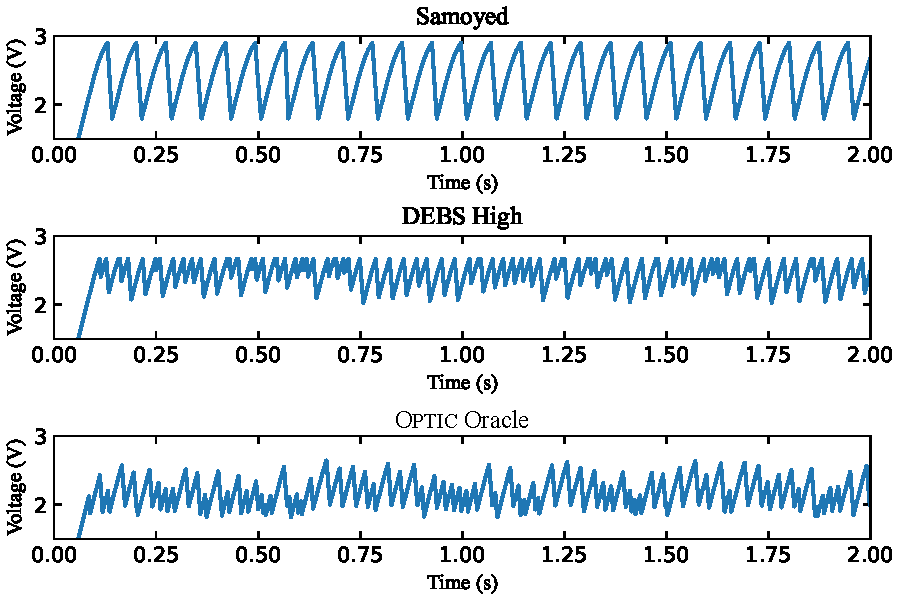
\includegraphics[width=0.9\columnwidth]{ch5_optic/figures/voltage_traces.pdf}
    \caption{An instance of supply voltage traces in simulation. }
    \label{fig:simulation_voltage}
\end{figure}

\begin{figure}
    \centering
    \begin{tikzpicture}
    \begin{axis}[
        width=0.8\columnwidth,height=5cm,
        ymin=0,ymax=50,
        xmin=0,xmax=60,
        xlabel={Capacitance Reduction},
        ylabel={No. of Completions},
        xticklabel={\pgfmathprintnumber\tick\%},
        xticklabel shift={3pt},
        legend style={
            anchor=south,
            at={(0.5,0.1)},
            legend columns=3,
        },
        ]
        \pgfplotstableread[col sep=comma]{ch5_optic/figures/exploration_results/cap.csv}{\mytable};
        \addplot 
            plot [Set1-A,mark=triangle*,dashed]
            table [x=cap_reduction,y=samoyed_perf] {\mytable};
        \addplot 
            plot [Set1-B,mark=square*,dashed]
            table [x=cap_reduction,y=debs_perf] {\mytable};
        \addplot 
            plot [Set1-C,mark=*,dashed]
            table [x=cap_reduction,y=repa_perf] {\mytable};
        \legend{Samoyed,\debs{} High,Adaptive}
    \end{axis}
    \end{tikzpicture}
    \caption{Number of completed operations of Samoyed,\debs{} High, and the Adaptive scheme with capacitance reduction. }
    \label{fig:simulation_cap}
\end{figure}

\fref{fig:simulation_cap} shows the results of the capacitance reduction test, where we have omitted \debs{} Low as it has already failed in non-termination with origin capacitance (so will still fail with reduced capacitance). 
With the capacitance decreased, \debs{} High also falls into non-termination like \debs{} Low. 
Samoyed, where its threshold is set to \SI{3.6}{\volt} in this case, can still progress until a 60\% reduction of capacitance because its abundant energy budget can support at least one or a few operations in one active cycle.
The adaptive scheme still maintains the highest forward progress among these control scheme. 


The above exploration presents that using a fixed low threshold can leave the system in non-termination (e.g. \debs{} Low and \debs{} High) but allocating an abundant energy budget compromises system efficiency (\debs{} High and Samoyed). 
An adaptive threshold can potentially overcome both problems.

Motivated by the previous examples of variable energy consumption and the benefit of an adaptive threshold, we propose \nn{}, a new methodology for profiling energy consumption of tasks at runtime and adapting energy budgets to the variable energy consumption of tasks. 
                 % Sec V
\section{Sizing under Real-World Energy Conditions} \label{sec:c4_demo}

In this section, we model an IPS with a photovoltaic (PV) energy harvester to explore the energy storage sizing effect in real-world energy conditions, and demonstrate use of the proposed sizing approach. 

\begin{figure}[!t]
    \centering
    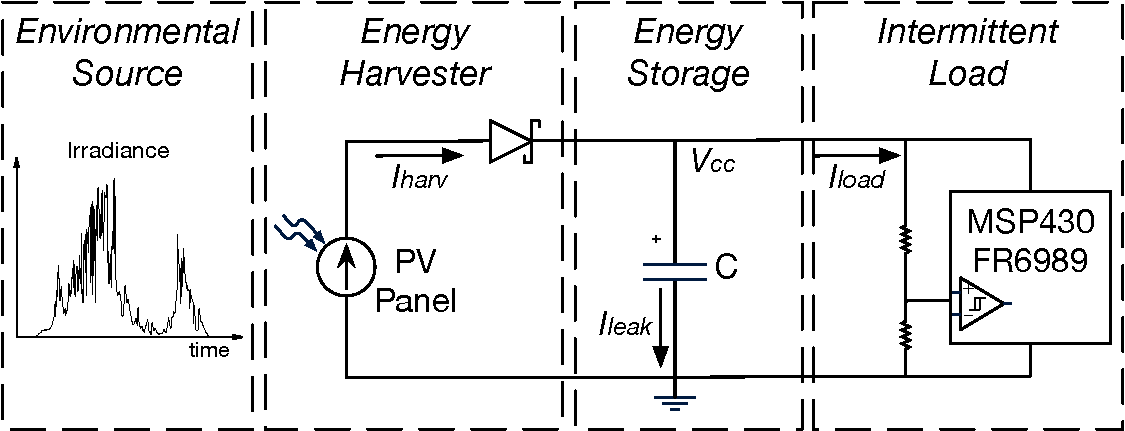
\includegraphics[width=\columnwidth]{ch4_sizingapproach/figures/solarmodel4}
    \caption{System model of a PV-based IPS.}
    \label{fig:Model}
\end{figure}

\subsection{Simulation Configuration}

We integrate the validated reactive IPS model into a system model with a PV energy-harvesting supply as shown in \figurename{~\ref{fig:Model}}. 
The energy storage model and the intermittent load model are as presented in \sref{sec:c3_exploration}. 

We use a converter-less supply circuit where only a Schottky diode is connected to the energy harvester output in order to prevent current backflow. 
The energy source conditions are imported from NREL outdoor solar irradiance data~\cite{stoffel1981nrel} and EnHANTs indoor irradiance data~\cite{6244798}. Four sets of light conditions are used to encompass different energy environments. 
To convert irradiance into harvested power, we adopt a PV cell model~\cite{en9050326} which uses the parameters available in common datasheets, so it can easily be reconfigured to suit various devices. 
The output current $I_{o}$ of the PV cell model can then be described as:
\begin{equation} \label{eq:pvcell}
    I_{o} = \frac{G}{G_{ref}} I_{sc} (1 - (1 - \frac{I_{mpp}}{I_{sc}}) ^ {\frac{V_{o}-V_{oc}}{V_{mpp} - V_{oc}}})
\end{equation}
where $V_{o}$ is the output voltage of the PV cell, $G$ is the ambient irradiance, $G_{ref}$ is the reference irradiance (normally 1000$W/m^2$), and $I_{sc}$, $V_{oc}$, $I_{mpp}$, $V_{mpp}$ are respectively short-circuit current, open-circuit voltage, and the current and voltage at maximum power point (MPP) given the reference irradiance. 
$V_{o}$ and $G$ are dynamic at run time, while other parameters in this model are constant. 
We refer to Panasonic Amorton glass type solar cells~\cite{solarcell} for PV cell properties as shown in Table~\ref{tab:pvcell}. We set four cells in series (with $V_{oc}$ = 3.56V) to match the operating voltage of the MCU (maximum 3.6V), and model energy harvester sizing by scaling the cell area. 


% A PV panel is an array of PV cells, which amplifies voltage and current output by connecting PV cells in series or parallel. In a PV panel, the open-circuit voltage is proportional to the number of cells in series, and the short-circuit current is proportional to the area of each cell and the number of cells in parallel. 

\begin{table}[!t]
    \renewcommand{\arraystretch}{1.2}
    \centering
    % \caption{PV Cell Properties under AM1.5 1000W/m$^2$ Light Conditions.}
    \caption{PV cell properties under a \SI{1000}{\watt\per\square\centi\meter}, AM-1.5 light source}
    \label{tab:pvcell}
    \begin{tabular}{|c|c|}
    \hline
    \textbf{Parameter} & \textbf{Value}\\
    \hline
    Open-Circuit Voltage & \SI{0.89}{\volt}/cell\\
    Short-Circuit Current & \SI{14.8}{\milli\ampere\per\square\centi\meter}\\
    Maximum Power Voltage & \SI{0.65}{\volt}/cell\\ 
    Maximum Power Current & \SI{12.1}{\milli\ampere\per\square\centi\meter}\\
    \hline
    \end{tabular}
\end{table}

Our simulation tool can perform two simulation processes: (a) sort and process the time distribution of environmental conditions, and (b) simulate system state chronologically with a fine-grained time step. 
Process (a) reduces simulation time significantly, e.g. from hours to seconds, but ignores the restore operation after a brownout reset, hence overestimating forward progress, and it overestimates more with smaller capacitance and lower supply current. 
In the following results, \figurename{~\ref{fig:harvstor}} come from Process (a) for fast exploration, and \figurename{~\ref{fig:interruption}} and \figurename{~\ref{fig:tradeoff}} come from Process (b) for accurate records. 

% Before the simulation, we developed and explored two simulation processes: (a) simulate system state chronologically with a fine-grained time step, and (b) sort energy source conditions into a distribution in time lengths and process the distribution. Process (b) shows a \SI{0.89}{\percent} mean absolute percentage error compared to Process (a), while reducing simulation time significantly (e.g. from several hours to several seconds in a one-year test). Hence, we use Process (b) in the following tests.

\subsection{Exploration with Real-World Energy Source Conditions} \label{subsec:harvstor}

% Goal: 
% 1. to show that this model can help designers to find a suitable size of EH to achieve their desired performance;
% 2. to show that sizing energy storage would have different degrees of impact on real deployment depending on the specific energy conditions;
% 3. demonstrate sizing approach. 

In real-world deployments, ambient energy source conditions are dependent on time and location. The energy harvester and storage need to be sized to achieve the desired forward progress across the range of expected conditions. 

\subsubsection{Sizing the Energy Harvester}

For the purposes of this exploration, three levels of baseline mean forward progress ($\alpha_{exe}$) are set as 0.1, 0.2, and 0.3. We use the system model to find the PV panel area that achieves the expected forward progress under the different energy source conditions with minimum energy storage. We scale the PV panel area to find that which achieves each baseline $\alpha_{exe}$. As shown in \figurename{~\ref{fig:harvstor}}, the energy harvester sizes that achieve the desired $\alpha_{exe}$ may span orders of magnitude given different energy source conditions from \SI{}{\square\milli\meter} for outdoor sources ((c) and (d)) to \SI{}{\square\centi\meter} for indoor sources ((a) and (b)). 
% To explore the energy harvester size needed for the above forward progress targets, we plot the forward progress against energy harvester size and energy storage capacitance in \figurename{~\ref{fig:harvstor}}. 

\subsubsection{Sizing the Energy Storage}

Having obtained the energy harvester sizes for the baseline forward progress, we then use the modelling approach to size energy storage.
% A table lists the PV panel area to achieve the target $\alpha_{exe}$ with minimum energy storage capacitance, the optimal capacitance with the forward progress improvement, and the alternative (decreased) PV panel area with the optimal capacitance. 
We analyse the sizing effect of energy storage on forward progress given real-world energy conditions. \figurename{~\ref{fig:harvstor}} shows a 7.8-43.3\% improvement in forward progress by sizing energy storage under the given real-world energy conditions and baseline energy harvester sizes. 
It can also be inferred that optimising energy storage can either improve forward progress for a given energy harvester size, or reduce the energy harvester size that achieves the target forward progress. Given higher-power energy sources (e.g. Denver 2018 and Hawaii 2018 outdoor solar), increasing the harvester size efficiently improves forward progress with minor dimensional overheads, e.g. tens of \SI{}{\square\milli\meter}; however, given lower-power sources (e.g. EnHANTs Setup~A and Setup~D indoor light), optimising energy storage capacitance can save tens of \SI{}{\square\centi\meter} of PV panel area to achieve the same forward progress.

% Also, the progress improvement by sizing energy storage varies accordingly with energy source conditions. This improvement stems from the reduction of restore and save overheads when the device works in the Intermittent mode, so this improvement becomes significant when the device works mostly in the Intermittent mode (typically when energy source is scarce, e.g. indoor source 1 and 2), and insignificant when the device works mostly in the On and Off modes (e.g. outdoor source 1 and 2). 

% \begin{figure}[!t]
%     \centering
%     \subfloat[EnHANTs Setup A]{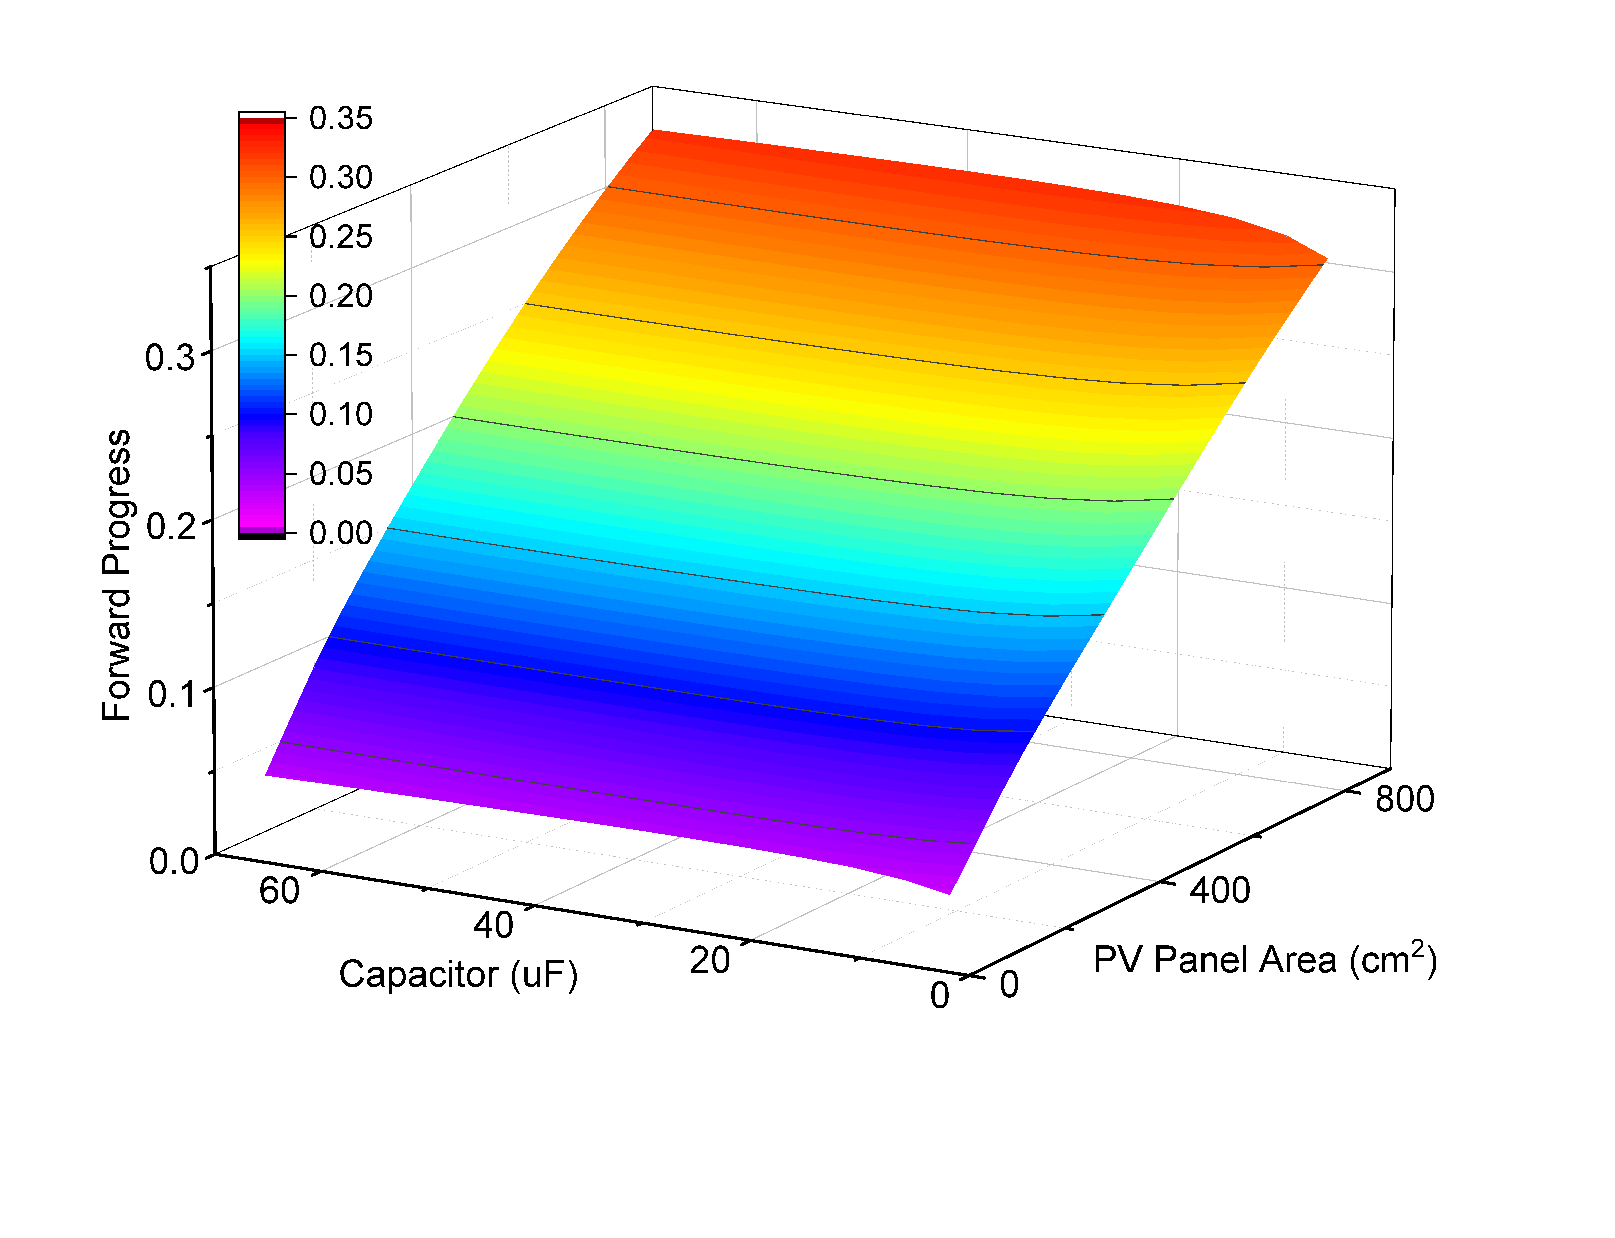
\includegraphics[width=1.65in]{HarvStor3DEnAFig}
%     \label{fig:harvstor1}}
%     \subfloat[EnHANTs Setup D]{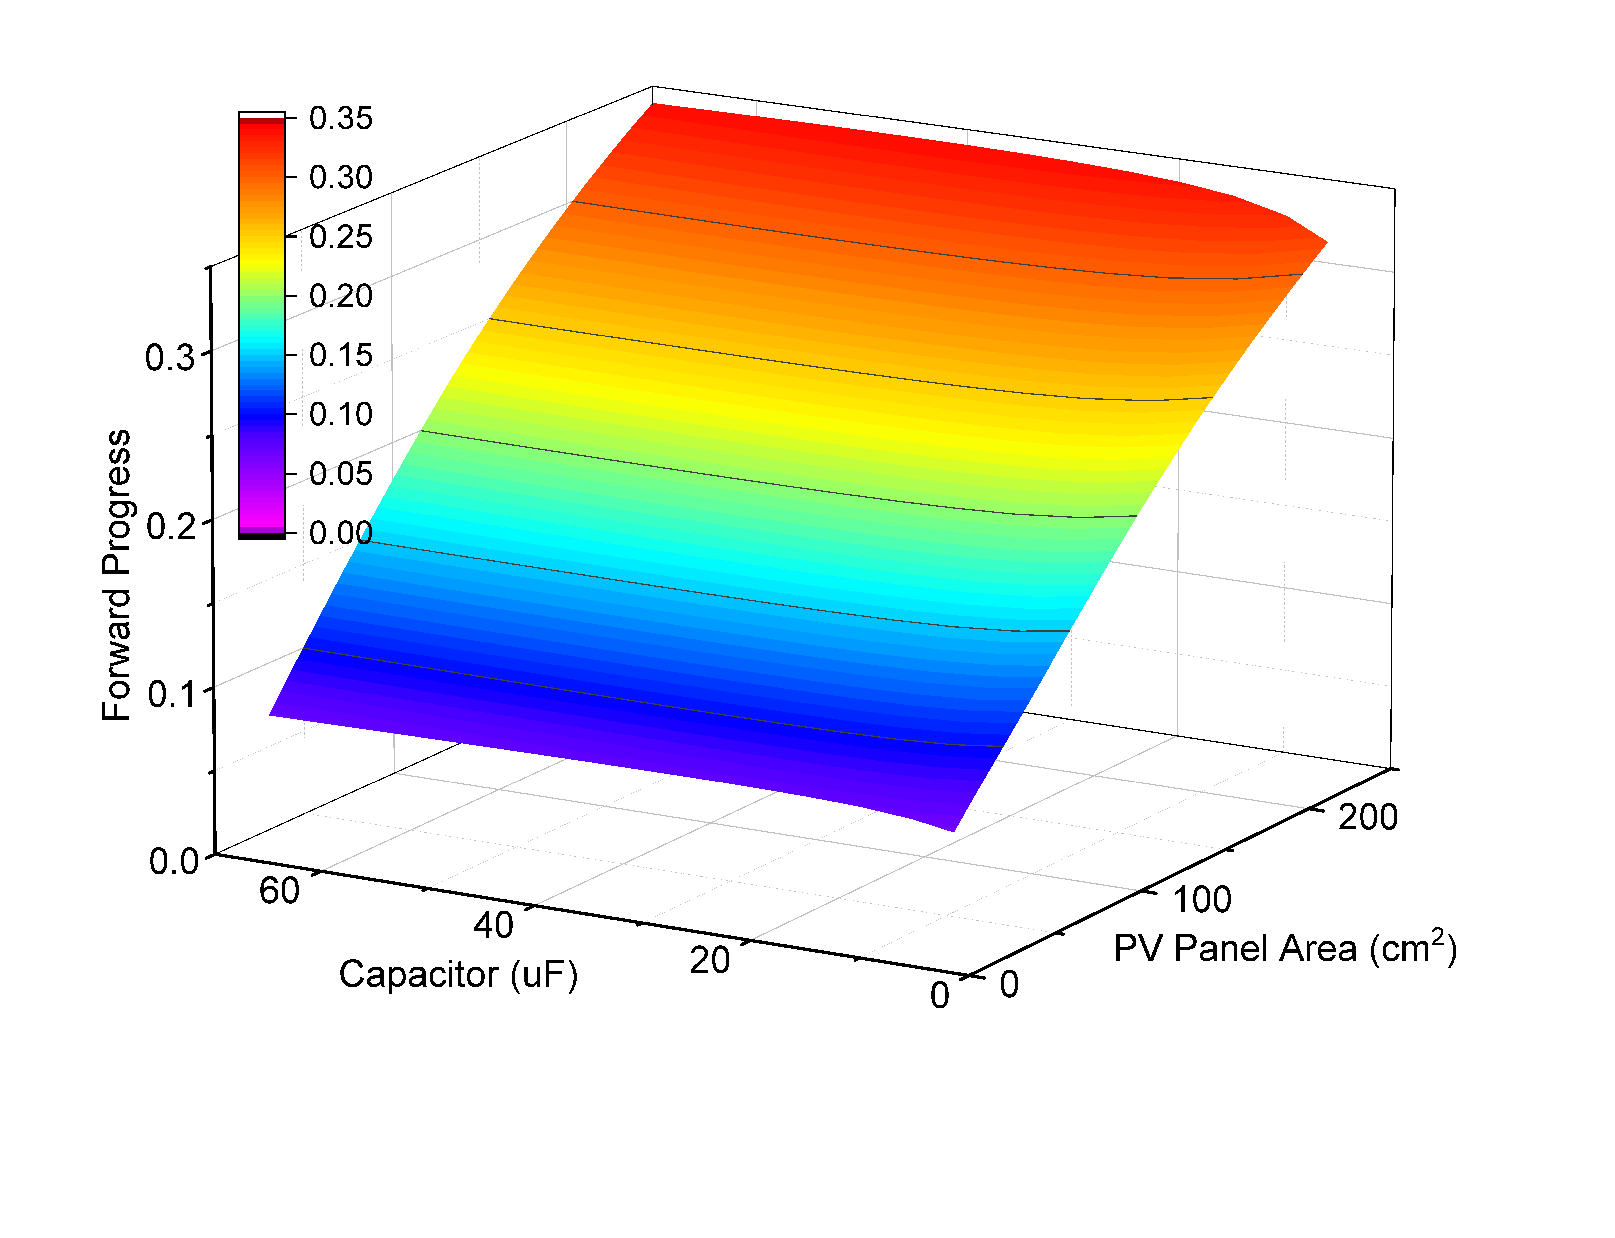
\includegraphics[width=1.65in]{HarvStor3DEnDFig}
%     \label{fig:harvstor2}}
%     \hfil
%     \subfloat[NREL Denver 2018]{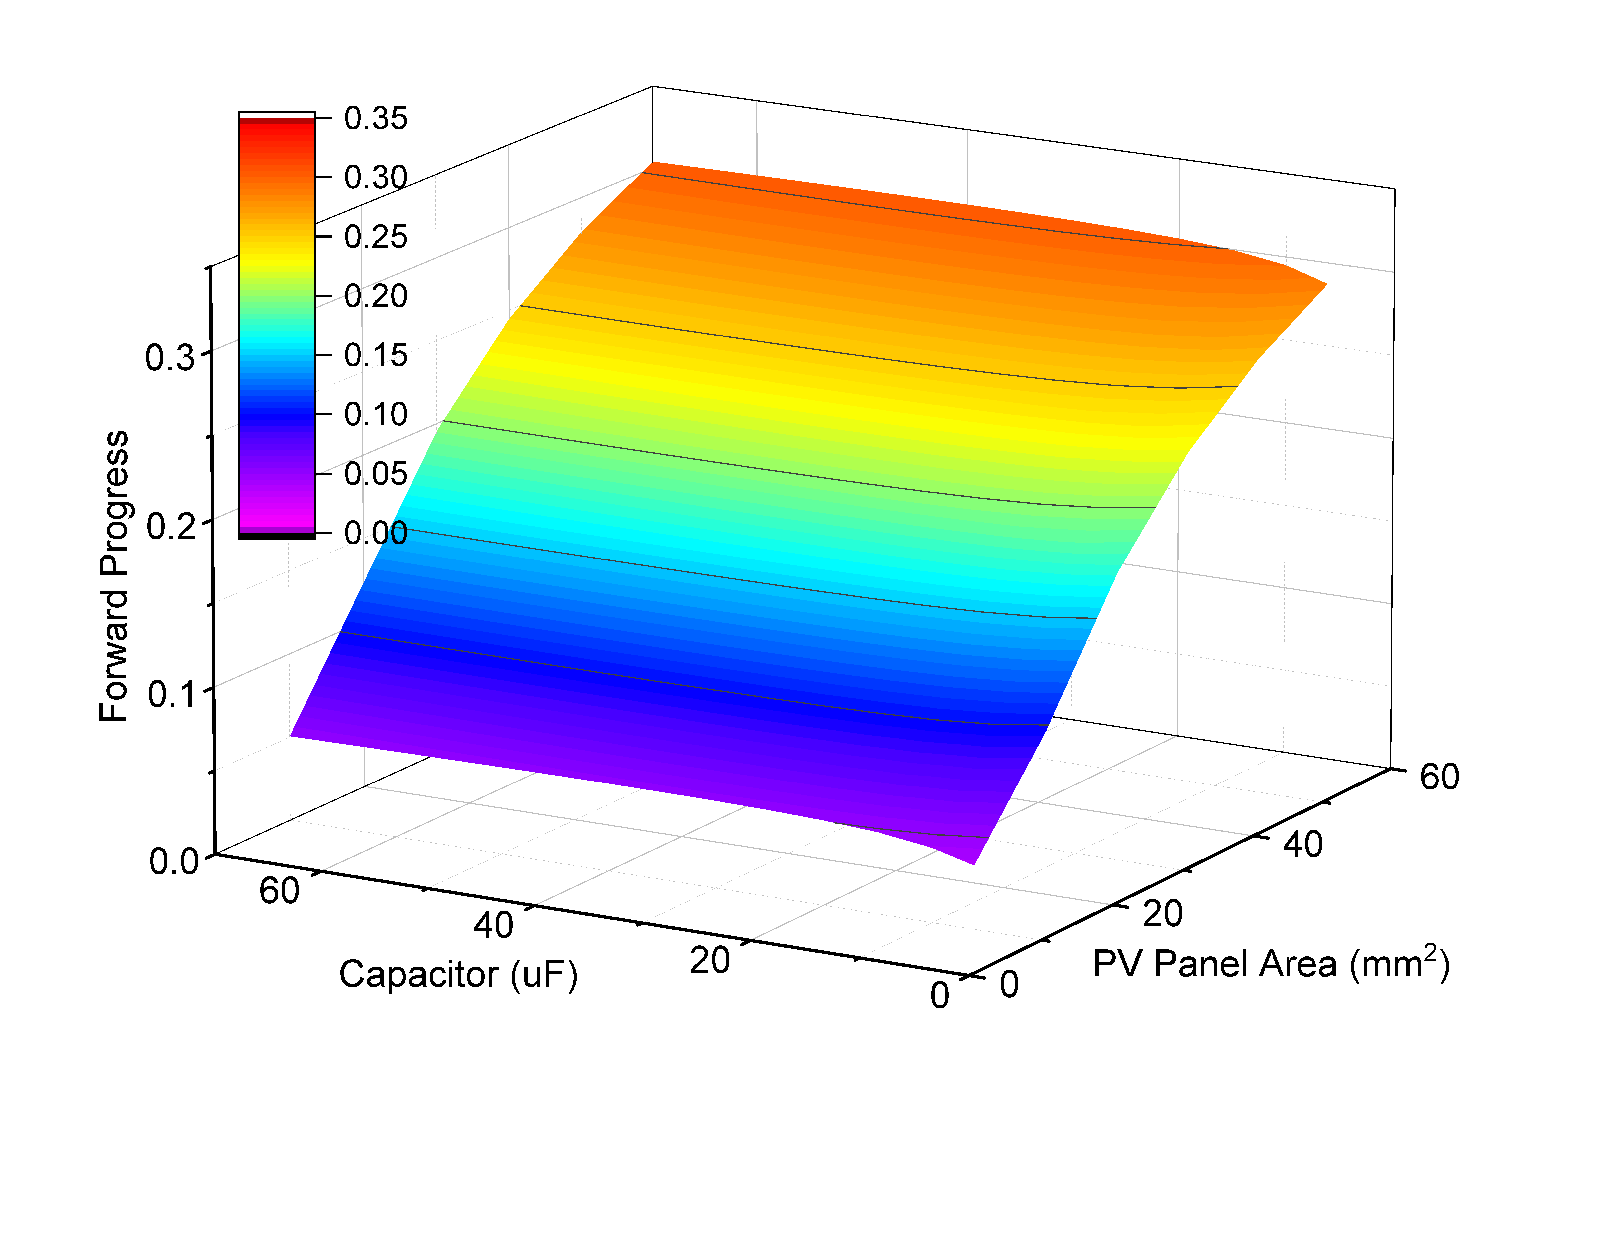
\includegraphics[width=1.65in]{HarvStor3DDenFig}
%     \label{fig:harvstor3}}
%     \subfloat[NREL Hawaii 2018]{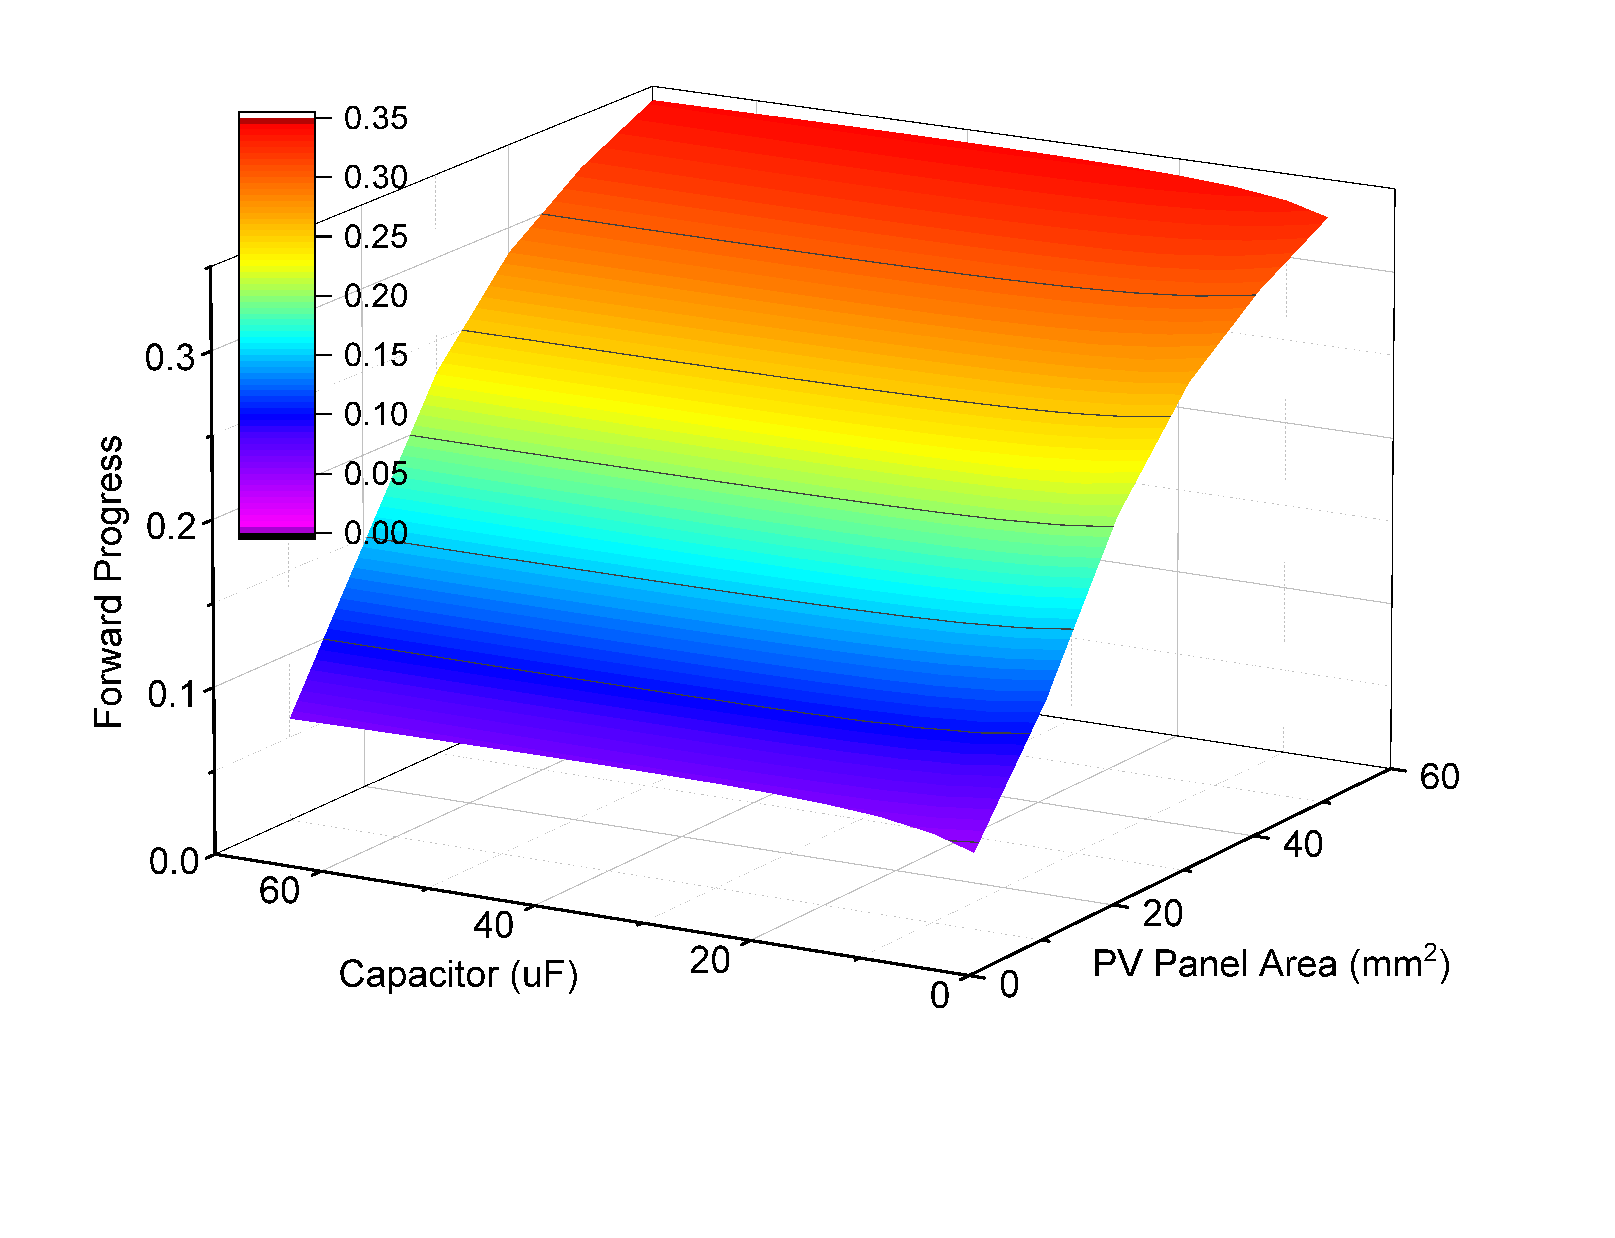
\includegraphics[width=1.65in]{HarvStor3DHawFig}
%     \label{fig:harvstor4}}
%     \caption{Forward progress against energy harvester size and energy storage capacitance in real-world energy source conditions.} 
%     \label{fig:harvstor}
% \end{figure}

\begin{figure}
    \centering
    \begin{subfigure}{0.49\columnwidth}
        \centering
        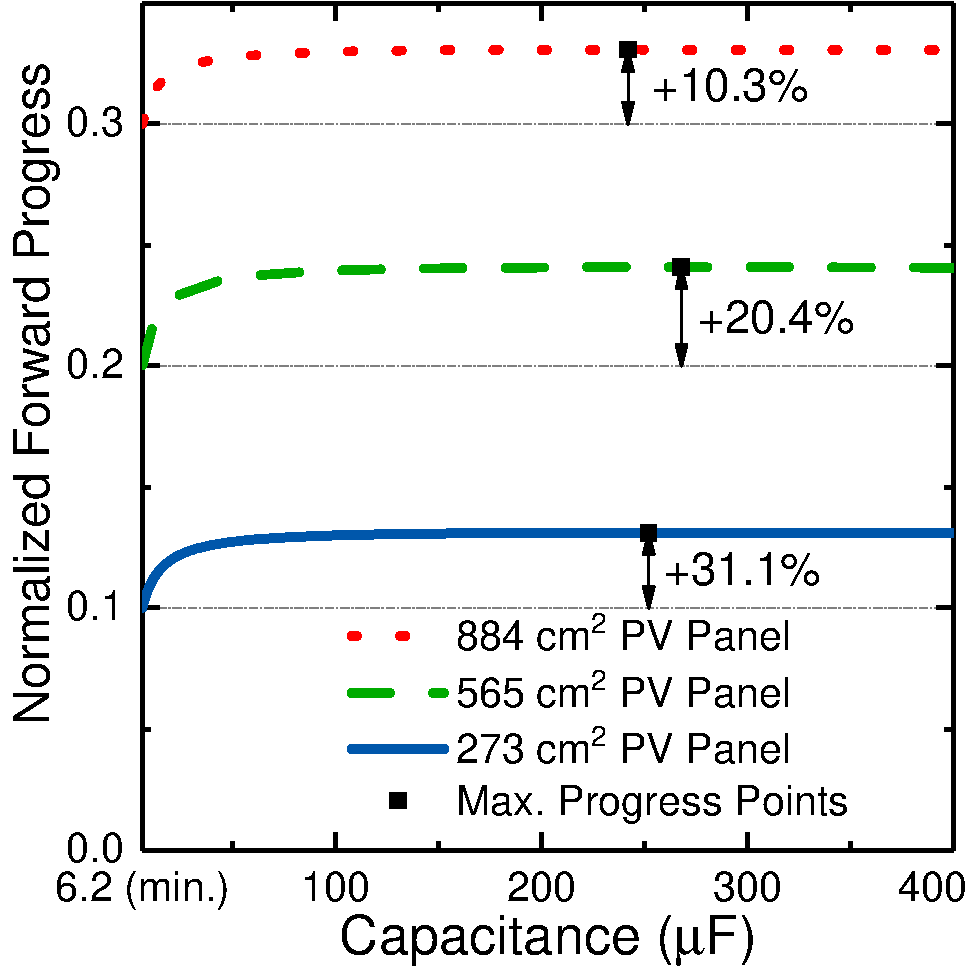
\includegraphics[width=\columnwidth]{ch4_sizingapproach/figures/HarvStorTgFig1}
        \caption{EnHANTs Setup A}
        \label{fig:harvstor1}
    \end{subfigure}
    \begin{subfigure}{0.49\columnwidth}
        \centering
        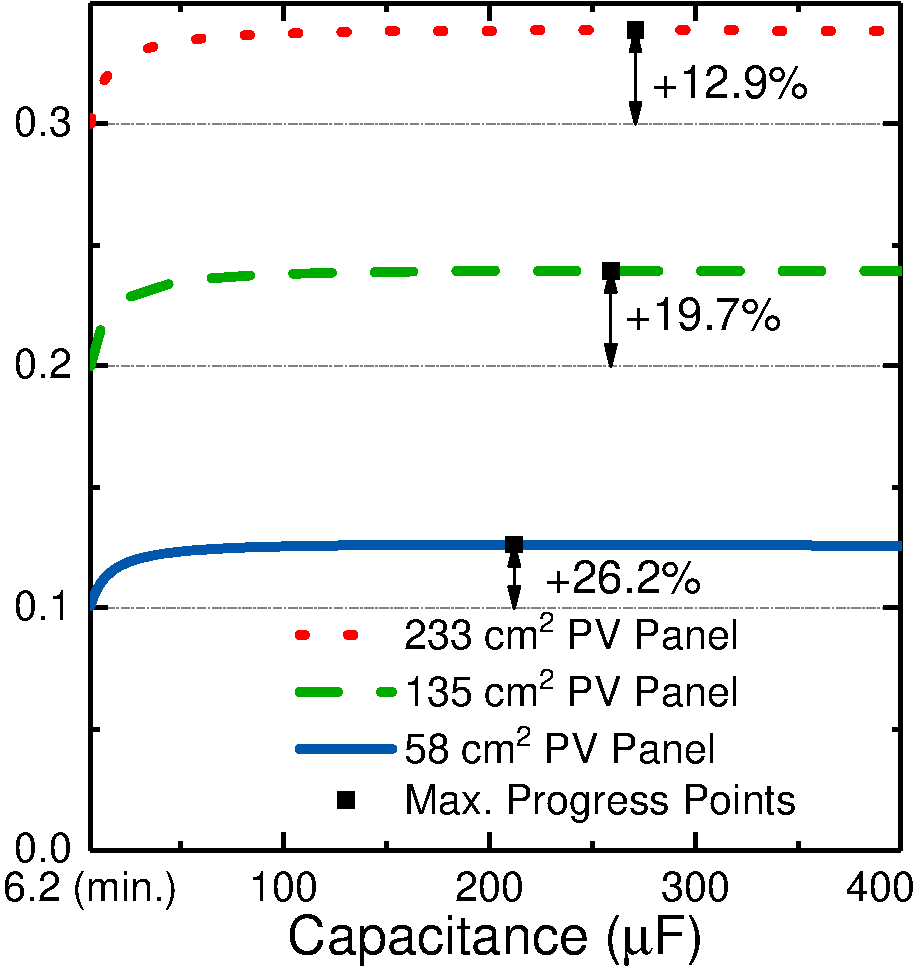
\includegraphics[width=\columnwidth]{ch4_sizingapproach/figures/HarvStorTgFig2}
        \caption{EnHANTs Setup D}
        \label{fig:harvstor2}
    \end{subfigure}
    \hfil
    \begin{subfigure}{0.49\columnwidth}
        \centering
        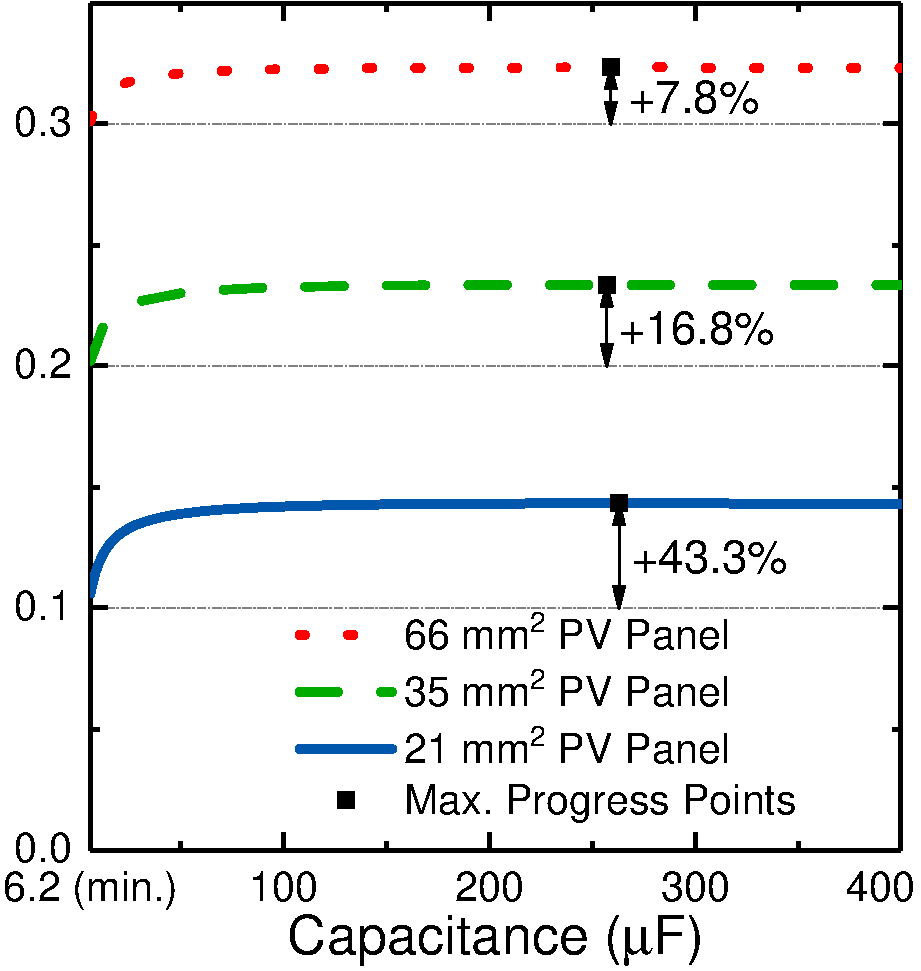
\includegraphics[width=\columnwidth]{ch4_sizingapproach/figures/HarvStorTgFig3}
        \caption{NREL Denver 2018}
        \label{fig:harvstor3}
    \end{subfigure}
    \begin{subfigure}{0.49\columnwidth}
        \centering
        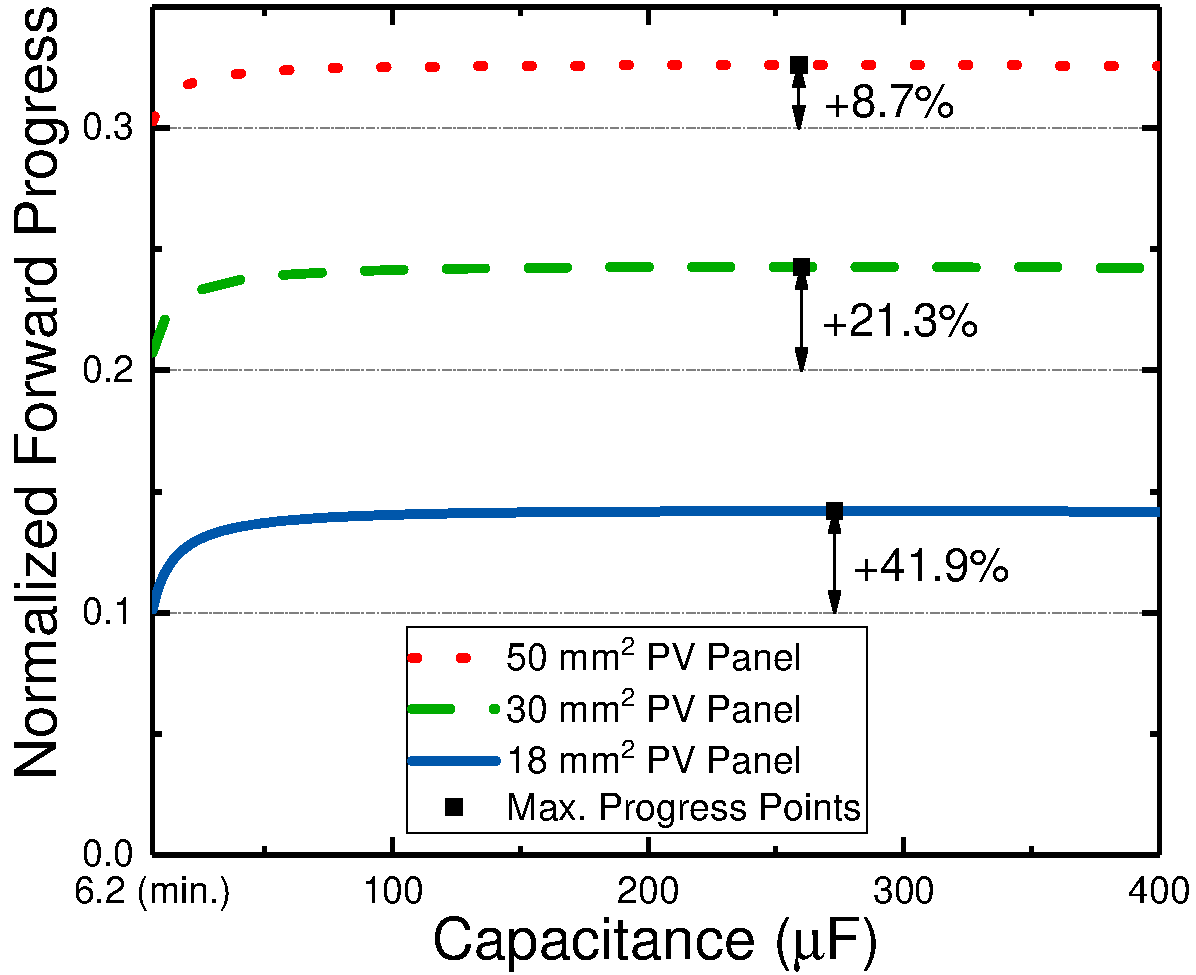
\includegraphics[width=\columnwidth]{ch4_sizingapproach/figures/HarvStorTgFig4}
        \caption{NREL Hawaii 2018}
        \label{fig:harvstor4}
    \end{subfigure}
    \caption{Improvement of average forward progress by sizing energy storage given different PV panel areas under real-world energy source conditions. The model is able to find the PV panel area required for achieving the target mean forward progress. } 
    \label{fig:harvstor}
\end{figure}

\todo[inline]{Adjust \fref{fig:harvstor} such that its font size is bigger and fills in more space, same with \fref{fig:harvstorrange}}

 The mean forward progress given target $\alpha_{exe}$ = 0.1 is plotted in \figurename{~\ref{fig:harvstorrange}}, with the 60th and 90th time percentiles of forward progress. In all the  above datasets, the energy source is absent and the system is off for around \SI{55}{\percent} of time, so we plot the percentiles from the 60th. The mean progress during the energy-available periods is averaged over the energy-absent periods, so the actual mean forward progress during the energy-available periods is nearly double the annual mean. 

% Absolute improvement are different? Large variations? What other results can I add? 
% The variations of forward progress are significant due to the large variations of energy source conditions, so practical implementation should consider such variation as .
% The improved progress during the energy-available periods is averaged over the energy-absent periods, so the actual amount of improvement when energy is available is higher than the mean. (wrong statement)

\begin{figure}
    \centering
    \begin{subfigure}{0.49\columnwidth}
        \centering
        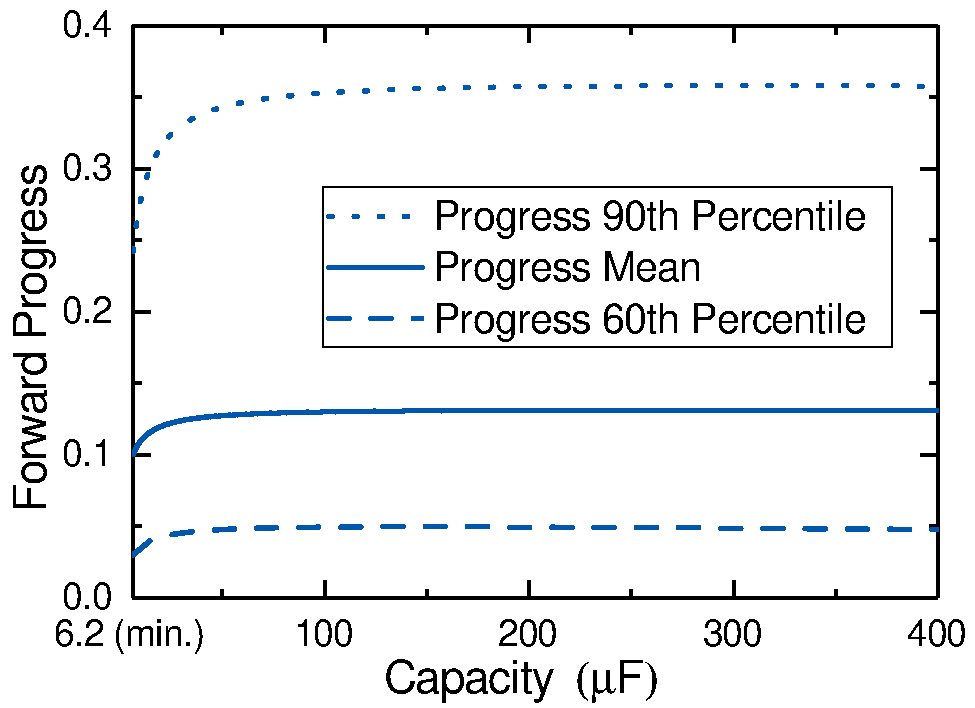
\includegraphics[width=\columnwidth]{ch4_sizingapproach/figures/HarvStorRan2Fig1}
        \caption{EnHANTs Setup A}
        \label{fig:harvstorrange1}
    \end{subfigure}
    \begin{subfigure}{0.49\columnwidth}
        \centering
        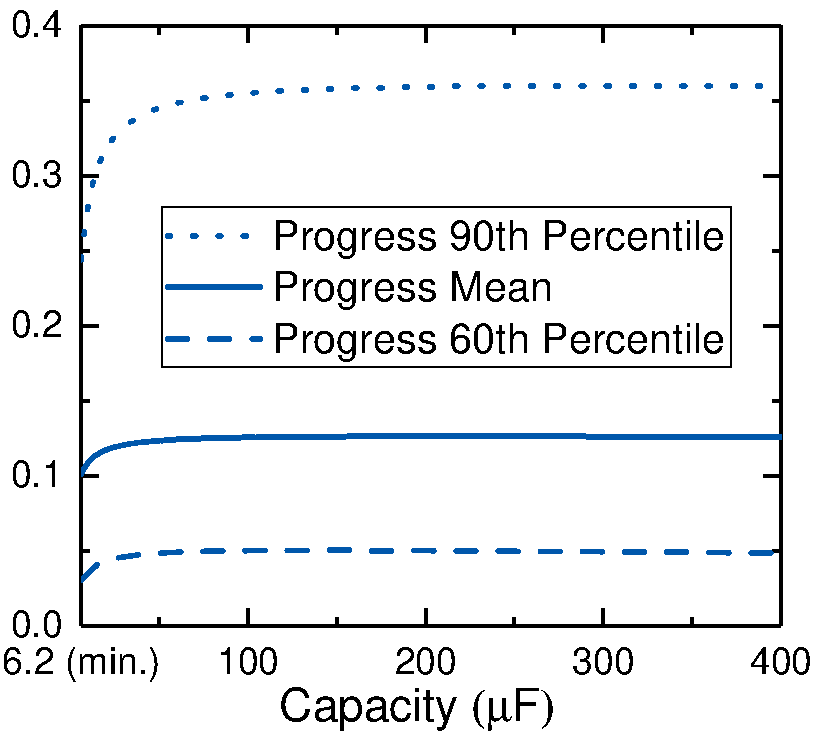
\includegraphics[width=\columnwidth]{ch4_sizingapproach/figures/HarvStorRan2Fig2}
        \caption{EnHANTs Setup D}
        \label{fig:harvstorrange2}
    \end{subfigure}
    \hfil
    \begin{subfigure}{0.49\columnwidth}
        \centering
        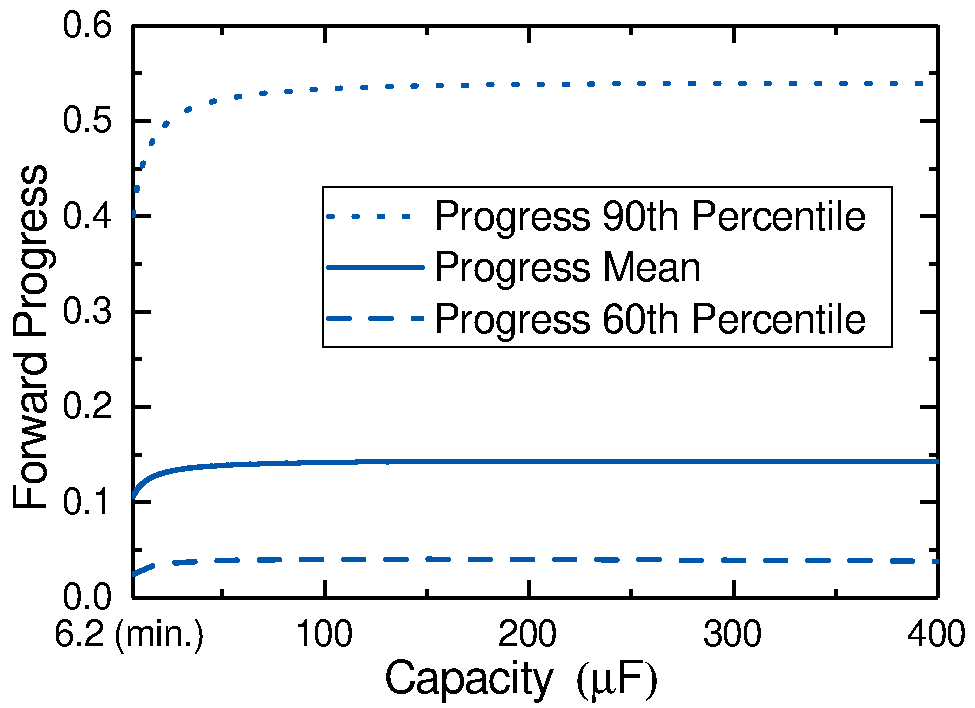
\includegraphics[width=\columnwidth]{ch4_sizingapproach/figures/HarvStorRan2Fig3}
        \caption{NREL Denver 2018}
        \label{fig:harvstorrange3}
    \end{subfigure}
    \begin{subfigure}{0.49\columnwidth}
        \centering
        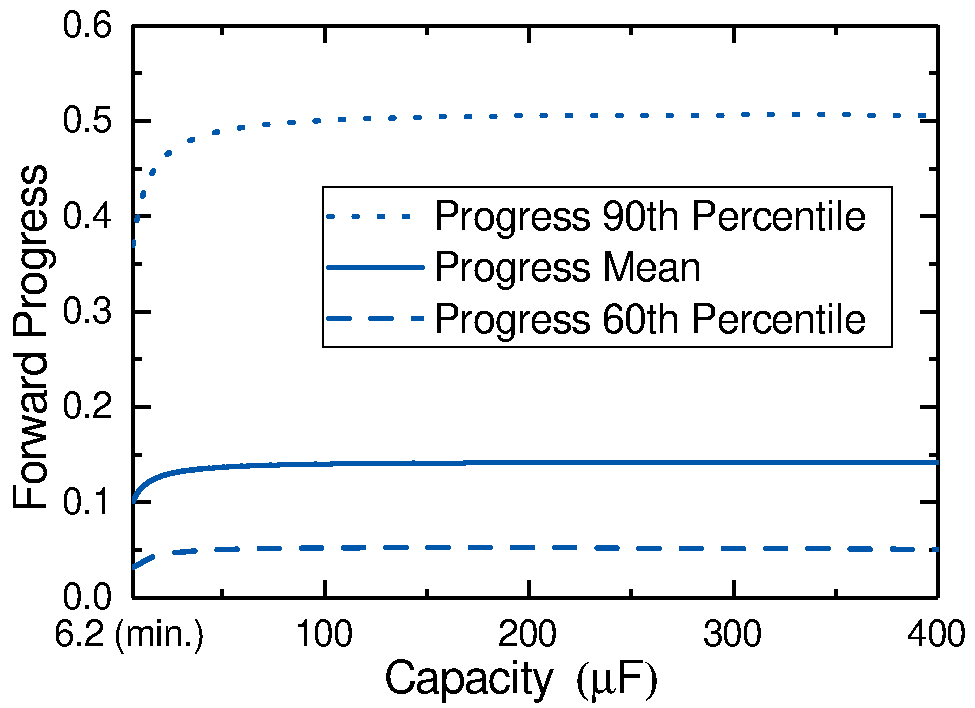
\includegraphics[width=\columnwidth]{ch4_sizingapproach/figures/HarvStorRan2Fig4}
        \caption{NREL Hawaii 2018}
        \label{fig:harvstorrange4}
    \end{subfigure}
    \caption{Time percentiles of forward progress by sizing energy storage with target $\alpha_{exe}$ = 0.1 and the corresponding PV panel area listed in \figurename{~\ref{fig:harvstor}}. The percentiles start from the 60th as the system is off for around \SI{55}{\percent} of time due to insufficient energy source. }
    \label{fig:harvstorrange}
\end{figure}

\subsubsection{Interruption Period} \label{subsubsec:intper}
Besides forward progress, we also explore how the capacitance can change the interruption periods. 
When interrupted by insufficient power supply, an IPS enters an interruption period where it saves its volatile state, waits for supply voltage to recover, and restores the state to resume execution, without making any forward progress. Applications that require frequent sensing may be negatively affected by long interruption periods. We measure an interruption period as \textit{the period between two successive execution periods}, e.g. a consecutive `SLR' period in \figurename{~\ref{fig:operatingCycle}} forms an interruption period. 
We record all the interruption periods during a one-year simulation with \SIrange{10}{50}{\micro\farad} capacitors, the Denver 2018 dataset, and an \SI{80}{\square\milli\meter} PV panel. 
\figurename{~\ref{fig:interruption}} presents the distribution of all the interruption periods. 
With increased energy storage, the interruption period is prolonged. For example, the 90th percentile of interruption periods increases from \SI{32.2}{\milli\second} at \SI{10}{\micro\farad} to \SI{123.4}{\milli\second} at \SI{50}{\micro\farad} at an approximate rate of \SI{23}{\milli\second} per \SI{10}{\micro\farad}. 
% The majority of the interruption periods are within \SI{200}{\milli\second}. 
Facilitated by the simulator, developers are enabled to estimate whether the distribution of interruption periods meet their application requirement. 

% Whether and how much this would affect  Time-sensitive applications may care 
% the total number of interruptions is reduced,


\begin{figure}
    \centering
    % \subfloat[a]{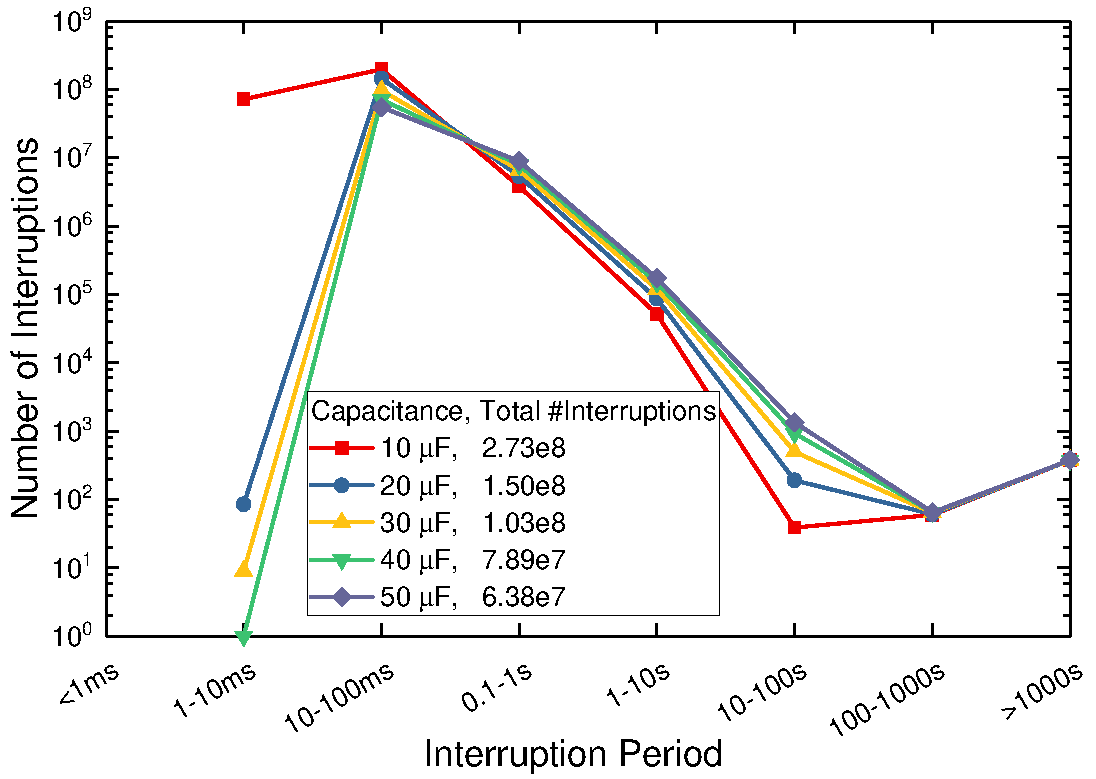
\includegraphics[width=2.8in]{IntPeriodFig}}
    % \label{fig:distribution}
    % \hfil
    \includegraphics[width=0.9\columnwidth]{ch4_sizingapproach/figures/IntPeriodOrdFig}
    \caption{Distribution of interruption periods. }
    \label{fig:interruption}
\end{figure}


% this will be a new one
% \begin{table}[!t]
%     \renewcommand{\arraystretch}{1.2}
%     \centering
%     \caption{Energy harvester size to achieve target $\alpha_{exe}$ with optimal energy storage capacitance to improve forward progress or reduce energy harvester size}
%     \label{tab:harvstornew}
%     \begin{tabular}{|cccc|}
%     \hline
%     \textbf{Target} & \textbf{PV Panel Area} & \textbf{Impr. of} $\pmb{\alpha_{exe}}$ & \textbf{Alternative} \\
%     $\pmb{\alpha_{exe}}$ & \textbf{w/ Min. C} & \textbf{w/ Opt. C} & \textbf{Panel Area / C} \\
%     % \multirow{2}{*}{\textbf{test}}
%     % \textbf{$T_{on}$} & \textbf{$T_{switch}$} \\ 
%     \hline 
%     \multicolumn{4}{|c|}{Indoor Source 1, EnHANTs Setup A} \\
%     \hline
%     % 0.1 & 277 cm$^2$ & 44 \textmu F / +22.3\% & 226 cm$^2$ / 42 \textmu F \\ 
%     % 0.2 & 570 cm$^2$ & 48 \textmu F / +15.2\% & 482 cm$^2$ / 48 \textmu F \\ 
%     % 0.3 & 891 cm$^2$ & 42 \textmu F / + 7.5\% & 802 cm$^2$ / 44 \textmu F \\ 
%     \hline
%     \multicolumn{4}{|c|}{Indoor Source 2, EnHANTs Setup D} \\
%     \hline
%     % 0.1 &  59 cm$^2$ & 37 \textmu F / +16.9\% &  49 cm$^2$ / 34 \textmu F \\
%     % 0.2 & 137 cm$^2$ & 45 \textmu F / +14.3\% & 116 cm$^2$ / 43 \textmu F \\
%     % 0.3 & 235 cm$^2$ & 47 \textmu F / + 9.6\% & 203 cm$^2$ / 47 \textmu F \\
%     \hline
%     \multicolumn{4}{|c|}{Outdoor Source 1, NREL Denver 2018} \\
%     \hline
%     % 0.1 & 21 mm$^2$ & 46 \textmu F / +26.3\% & 18 mm$^2$ / 45 \textmu F \\
%     % 0.2 & 35 mm$^2$ & 45 \textmu F / +11.6\% & 31 mm$^2$ / 45 \textmu F \\
%     % 0.3 & 66 mm$^2$ & 45 \textmu F / + 5.5\% & 58 mm$^2$ / 45 \textmu F \\
%     % \hline
%     \multicolumn{4}{|c|}{Outdoor Source 2, NREL Hawaii 2018} \\
%     \hline
%     % 0.1 & 19 mm$^2$ & 48 \textmu F / +28.7\% & 16 mm$^2$ / 46 \textmu F \\
%     % 0.2 & 30 mm$^2$ & 45 \textmu F / +12.9\% & 27 mm$^2$ / 46 \textmu F \\
%     % 0.3 & 50 mm$^2$ & 45 \textmu F / + 5.8\% & 45 mm$^2$ / 45 \textmu F \\
%     \hline
%     \end{tabular} 
% \end{table}

% \begin{table}[!t]
%     \renewcommand{\arraystretch}{1.2}
%     \centering
%     \caption{Sizing energy harvester and energy storage in real-world energy source conditions}
%     \label{tab:harvstor}
%     \begin{tabular}{cccc}
%     \hline
%     \textbf{PV Panel Area} & \textbf{Opt. C} & \textbf{Exe. Time Ratio} & \textbf{Impr. on Min. C} \\
%     % \textbf{$T_{on}$} & \textbf{$T_{switch}$} \\ 
%     \hline 
%     \multicolumn{4}{c}{Outdoor Source 1, NREL 2018 Hawaii} \\
%     \hline
%     20 mm$^2$ & 47 \textmu F & 0.147 & 27.2 \% \\
%     40 mm$^2$ & 45 \textmu F & 0.286 & 7.8 \% \\
%     60 mm$^2$ & 43 \textmu F & 0.342 & 4.6 \% \\
%     80 mm$^2$ & 45 \textmu F & 0.373 & 3.3 \% \\
%     \hline
%     \multicolumn{4}{c}{Outdoor Source 2, NREL 2018 Denver} \\
%     \hline
%     20 mm$^2$ & 45 \textmu F & 0.124 & 27.8 \% \\
%     40 mm$^2$ & 44 \textmu F & 0.246 & 9.7 \% \\
%     60 mm$^2$ & 44 \textmu F & 0.305 & 6.0 \% \\
%     80 mm$^2$ & 44 \textmu F & 0.339 & 4.6 \% \\
%     \hline
%     \multicolumn{4}{c}{Indoor Source 1, EnHANTs Setup D} \\
%     \hline
%     20 cm$^2$ & 26 \textmu F & 0.052 & 11.9\% \\
%     40 cm$^2$ & 31 \textmu F & 0.088 & 14.6\% \\
%     60 cm$^2$ & 36 \textmu F & 0.119 & 17.0\% \\
%     80 cm$^2$ & 37 \textmu F & 0.150 & 17.3\% \\
%     \hline
%     \multicolumn{4}{c}{Indoor Source 2, EnHANTs Setup A} \\
%     \hline
%     100 cm$^2$ & 31 \textmu F & 0.036 & 33.6\% \\
%     200 cm$^2$ & 39 \textmu F & 0.088 & 25.1\% \\
%     300 cm$^2$ & 44 \textmu F & 0.132 & 21.9\% \\
%     400 cm$^2$ & 47 \textmu F & 0.170 & 19.7\% \\
%     \hline
%     \end{tabular} 
% \end{table}

% \begin{table}[!t]
%     \renewcommand{\arraystretch}{1.2}
%     \centering
%     \caption{Energy harvester size to achieve target $\alpha_{exe}$ with optimal energy storage capacitance to improve forward progress or reduce energy harvester size}
%     \label{tab:harvstornew}
%     \begin{tabular}{|cccc|}
%     \hline
%     \textbf{Target} & \textbf{PV Panel Area} & \textbf{Impr. of} $\pmb{\alpha_{exe}}$ & \textbf{Alternative} \\
%     $\pmb{\alpha_{exe}}$ & \textbf{w/ Min. C} & \textbf{w/ Opt. C} & \textbf{Panel Area / C} \\
%     % \multirow{2}{*}{\textbf{test}}
%     % \textbf{$T_{on}$} & \textbf{$T_{switch}$} \\ 
%     \hline 
%     \multicolumn{4}{|c|}{Indoor Source 1, EnHANTs Setup A} \\
%     \hline
%     0.1 & 277 cm$^2$ & 44 \textmu F / +22.3\% & 226 cm$^2$ / 42 \textmu F \\ 
%     0.2 & 570 cm$^2$ & 48 \textmu F / +15.2\% & 482 cm$^2$ / 48 \textmu F \\ 
%     0.3 & 891 cm$^2$ & 42 \textmu F / + 7.5\% & 802 cm$^2$ / 44 \textmu F \\ 
%     \hline
%     \multicolumn{4}{|c|}{Indoor Source 2, EnHANTs Setup D} \\
%     \hline
%     0.1 &  59 cm$^2$ & 37 \textmu F / +16.9\% &  49 cm$^2$ / 34 \textmu F \\
%     0.2 & 137 cm$^2$ & 45 \textmu F / +14.3\% & 116 cm$^2$ / 43 \textmu F \\
%     0.3 & 235 cm$^2$ & 47 \textmu F / + 9.6\% & 203 cm$^2$ / 47 \textmu F \\
%     \hline
%     \multicolumn{4}{|c|}{Outdoor Source 1, NREL Denver 2018} \\
%     \hline
%     0.1 & 21 mm$^2$ & 46 \textmu F / +26.3\% & 18 mm$^2$ / 45 \textmu F \\
%     0.2 & 35 mm$^2$ & 45 \textmu F / +11.6\% & 31 mm$^2$ / 45 \textmu F \\
%     0.3 & 66 mm$^2$ & 45 \textmu F / + 5.5\% & 58 mm$^2$ / 45 \textmu F \\
%     \hline
%     \multicolumn{4}{|c|}{Outdoor Source 2, NREL Hawaii 2018} \\
%     \hline
%     0.1 & 19 mm$^2$ & 48 \textmu F / +28.7\% & 16 mm$^2$ / 46 \textmu F \\
%     0.2 & 30 mm$^2$ & 45 \textmu F / +12.9\% & 27 mm$^2$ / 46 \textmu F \\
%     0.3 & 50 mm$^2$ & 45 \textmu F / + 5.8\% & 45 mm$^2$ / 45 \textmu F \\
%     \hline
%     \end{tabular} 
% \end{table}

% \begin{table}[!t]
%     \renewcommand{\arraystretch}{1.2}
%     \centering
%     \caption{PV panel area to achieve different $·\alpha_{exe}$ with minimum energy storage}
%     \label{tab:sizeharv}
%     \begin{tabular}{|c|ccc|}
%     \hline 
%     % \textbf{Dataset} & \multicolumn{3}{c}{\textbf{PV Panel Area}} \\
%     % \textbf{Dataset} & \textbf{PV Panel Area} & \textbf{Actual Exe. Time Ratio} \\
%     \textbf{Dataset} & \textbf{$\alpha_{exe}$} = 0.1 & $\alpha_{exe}$ = 0.2 & $\alpha_{exe}$ = 0.3 \\
%     \hline
%     EnHANTs A (Indoor)  & 277 cm$^2$ & 570 cm$^2$ & 891 cm$^2$ \\
%     EnHANTs D (Indoor)  &  59 cm$^2$ & 137 cm$^2$ & 235 cm$^2$ \\
%     Denver 2018 (Outdoor) &  21 mm$^2$ &  35 mm$^2$ &  66 mm$^2$ \\
%     Hawaii 2018 (Outdoor) &  19 mm$^2$ &  30 mm$^2$ &  50 mm$^2$ \\
%     \hline
%     \end{tabular} 
% \end{table}

\subsection{Trading Forward Progress, Dimensions, and Interruption Period} \label{subsec:tradeoff}

% Prior intermittent computing approaches adopt only the minimum energy storage capacitance so as to minimise device dimensions and interruption periods. 

Although increasing energy storage capacitance improves forward progress, larger capacitance increases both dimensions and interruption periods. We evaluate the overheads of increased capacitor dimensions and interruption periods, and then trade them off against forward progress using a cost function to suggest an optimal capacitance value. 
% We evaluate this impact

\subsubsection{Metric of Dimensions}

The overhead of capacitor dimensions is evaluated by characteristics of off-the-shelf tantalum capacitors. We narrow down the range of sample capacitors within a set of characteristics: low-profile, 10V rated voltage, and surface-mount package, and select six series of capacitors\footnote{The series of capacitor considered were: AVX TAJ, AVX TACmicrochip, AVX F92, Vishay 572D, Vishay 591D, and Vishay 592D.}. The volume and capacitance of these devices are plotted in \figurename{~\ref{fig:capvol}}. We use the regression of these data to approximate a capacitance-volume relationship.
% ~\cite{tancap1, tancap2, tancap3, tancap4, tancap5, tancap6}
% Among the common capacitor chemistries with \textmu F to mF capacitance, tantalum capacitors manifest low leakage 

\begin{figure}
    \centering
    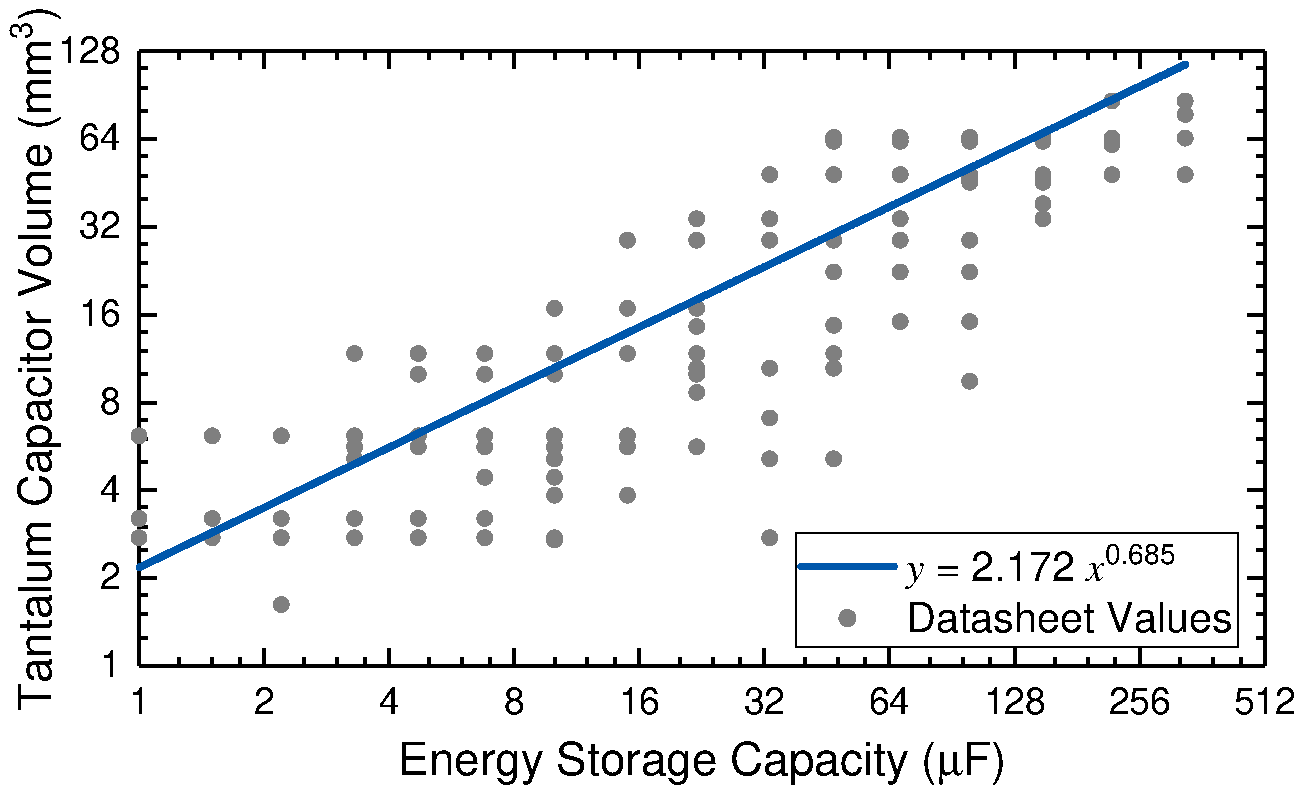
\includegraphics[width=0.9\columnwidth]{ch4_sizingapproach/figures/CapVol2Fig2}
    \caption{Tantalum capacitor volume against capacitance for the six series of capacitors analysed. }
    \label{fig:capvol}
\end{figure}

\subsubsection{Metric of Interruption Periods}

% Definition/Measurement of interruption periods. recharging ability? Considering leakage?
% why interruption periods is important, why we consider it.

% , i.e. the period that does not make forward progress. The total interruption periods should be opposite to forward progress. 
Applications may have various requirements on interruption periods. To demonstrate the usage of our sizing approach, we consider a designer requests the 90th percentile of all interruption periods as an example metric of interruption periods, denoted as $T_{int}$. This metric indicates 90\% of interruption periods are shorter than $T_{int}$. This metric can be adapted for particular application requirements. 
% In We assume that $T_{interrupt}$ is preferable to be short for general application. 

% metric of interruption periods 
% Technically, the actual inactive period between two active periods depends on capacitance, the start and end voltage of recharging, and the current input and consumption. While the end voltage (restore voltage) and current consumption can be set or predicted, the start voltage and current flows vary with energy source conditions. Instead of evaluating the inactive period in complex conditions, we use the time between two successive execution intervals given \SI{0.5}{\milli\ampere} supply current in the Intermittent mode as a metric of interruption periods (or recharging ability). Using eqs.~(\ref{eq:texe}) and (\ref{eq:tperiod}), we can obtain this recharging period between two successive execution intervals in the Intermittent mode as: 

% \begin{equation}
%     \begin{aligned}
%         T_{recharge} = & \quad T_{period} - T_{exe} \\
%         = & \quad \frac{C(V_{r} - V_{s}) + T_{s}(I_{in} - I_{s})}{I_{in} - I_{lpm}} + T_{r}
%     \end{aligned}
% \end{equation}

\subsubsection{Cost Function}

From the previous observations (\figurename{~\ref{fig:maxfwp}}) we can see that achieving the optimal progress improvement costs much more capacitance (mean 3.2$\times$) than to achieve 95\% improvement. A trade-off is necessary to improve forward progress while restricting the overheads of increased capacitor volume and interruption periods. We use the cost function in (\ref{eq:tradeoff}) to trade off forward progress, capacitor volume, and interruption periods: 
\begin{equation}
    f = \frac{\alpha_{exe}}{k_1} - \left(\frac{v_{cap}}{k_2}\right) ^ {2} - \left(\frac{T_{int}}{k_3}\right) ^ {2} 
    \label{eq:tradeoff}
\end{equation}
where $v_{cap}$ denotes capacitor volume and $T_{int}$ denotes interruption periods. $\alpha_{exe}$, $v_{cap}$, $T_{int}$ can be described as functions of $C$. $k_1$, $k_2$, and $k_3$ are independent factors used for normalising each metric, and they are empirically determined according to applications. In this example, the undesirable parameters are expressed as quadratics to give an increasing cost to higher values. While only three parameters are considered here, others (such as the energy harvester size) could be included for a system-wise sizing scenario.
% $\alpha_{exe}$ denotes normalized forward progress,
% ; they can all be described as functions of $C$
% , so comparing them is meaningless, e.g. $\frac{1}{k_1} / \frac{1}{k_2} = 1000$ does not mean that forward progress is 1000 times more important than capacitor volume in this cost function.
% We configure the function by setting $k_1$ = 0.2, $k_2$ = 200, and $k_3$ = 1, where $v_{cap}$ is in \SI{}{\cubic\milli\meter} and $T_{recharge}$ is in s.
As an example, we configure the function by setting $k_1$ = 0.2, $k_2$ = \SI{200}{\cubic\milli\meter}, and $k_3$ = \SI{500}{\milli\second}. 
%, i.e.:
%\begin{equation}
%    f = \frac{\alpha_{exe}}{0.2} - (\frac{v_{cap}}{200}) ^ {2} - T_{recharge} ^ {2} 
%    \label{eq:tradeoffuse}
%\end{equation}
% where $v_{cap}$ is in \SI{}{\cubic\milli\meter} and $T_{recharge}$ is in second. Here, $\frac{1}{k_1} / \frac{1}{k_2}$ equals 1000, but this does not mean that forward progress is 1000 times more important than capacitor volume.

\subsubsection{Results}

The effect of the trade-off is plotted in \figurename{~\ref{fig:tradeoff}} using the Denver 2018 energy source dataset. Compared to the capacitor size that solely maximises forward progress, on average, an appropriately-sized capacitor achieves 93\% of the maximum forward progress, while saving 83\% of capacitor volume and 91\% of interruption periods. Compared to the minimum storage case, the appropriately-sized capacitor improves forward progress by 12-124\% with energy storage increased from \SI{6.2}{\micro\farad} to \SI{30}{\micro\farad}.

\begin{figure}
    \centering
    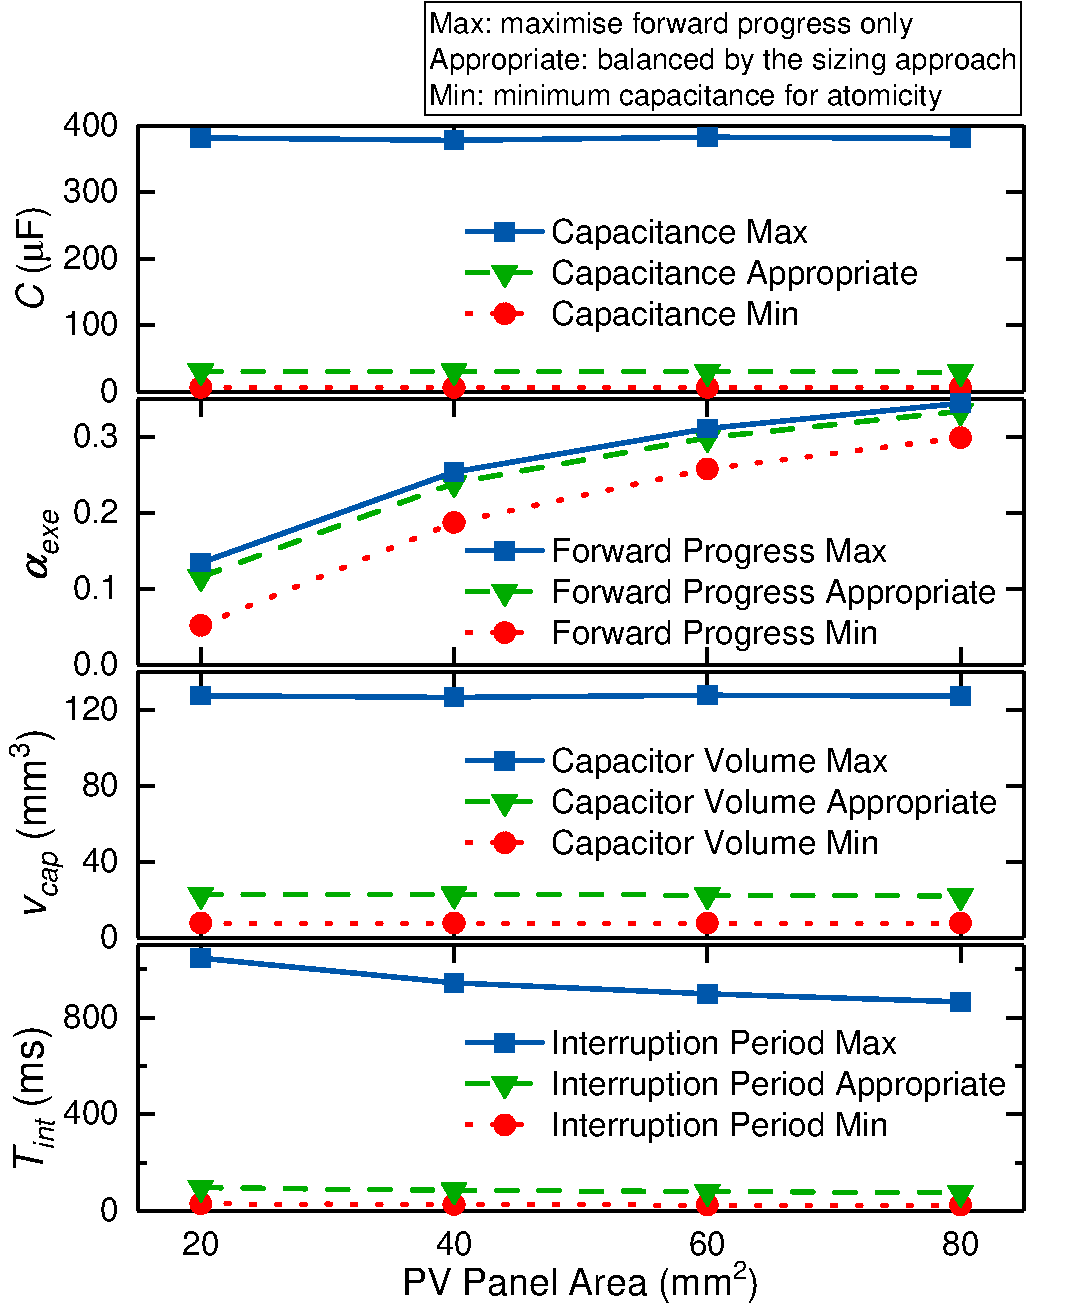
\includegraphics[width=\columnwidth]{ch4_sizingapproach/figures/Tradeoff3Fig}
    \caption{The sizing approach trades off forward progress, capacitor volume, and interruption periods. The results are plotted against a range of PV panel area, given Denver 2018 energy source dataset. }
    \label{fig:tradeoff}
\end{figure}

As shown in \figurename{~\ref{fig:capvol}}, the closest available capacitance that satisfies the \SI{6.2}{\micro\farad} minimum capacitance is \SI{6.8}{\micro\farad}, whereas the closest available capacitance to the appropriate \SI{30}{\micro\farad} is \SI{33}{\micro\farad}. The minimum volumes of \SI{6.8}{\micro\farad} and \SI{33}{\micro\farad} capacitors are both \SI{2.75}{\cubic\milli\meter}, which means using the appropriate capacitance, instead of the minimum one, may not incur dimensional overhead. 
% For \SI{47}{\micro\farad}, the absolute volume (\SI{5.12}{\cubic\milli\meter}) is insignificant compared to the device as a whole, e.g. an MSP430FR6989 MCU chip alone occupies \SI{274.4}{\cubic\milli\meter} (14 $\times$ 14 $\times$ 1.4). 
The regressed volume of the above two capacitance values are \SI{8.1}{\cubic\milli\meter} and \SI{23.8}{\cubic\milli\meter} respectively. However, the selection of capacitors can be dependent on factors other than physical volume, such as reliability, operation temperature, and more specific application needs. These factors can also be added into the cost function if necessary. 
% Again, such a volume scale is still insignificant in a whole device. 

                  % Sec VII

%%%%%%%%%%%%%%%%%%%%%%%%%%%%%%%%%%%%%%%%%%%%%%%%%%%%%%%%%%
%%% Section VIII: Conclusion
%%%%%%%%%%%%%%%%%%%%%%%%%%%%%%%%%%%%%%%%%%%%%%%%%%%%%%%%%%

\section{Conclusions} \label{section:conclusion}

% We explored the relationship between forward progress and energy storage capacitance in intermittent computing through a theoretical model.

% In this paper, we presented a model of reactive ICSs that accurately estimates forward progress. 
% Using this model, we explored the sizing effect of energy storage on forward progress with respect to supply current and volatile state size, showing up to \SI{64.9}{\percent} progress improvement under constant current supply and \SIrange{7.8}{43.3}{\percent} improvement on annual mean forward progress 
% under various real-world energy conditions. 

While conventional ICSs have used minimal levels of capacitance, this paper has shown that increasing the amount of energy storage can improve system performance by up to 65\% with a constant current supply and 43\% with real-world PV sources. The work includes a simulation tool which is available to download, enabling researchers to experiment with energy storage sizes to optimize ICS designs. A cost function can be incorporated, allowing various aspects of system performance to be traded-off. Our conclusion is that energy storage should be carefully designed, rather than minimized or indiscriminately picked, to efficiently operate ICSs.
%\color{blue}
%\todo{Alex to update this after other parts completed/queries resolved.}In this paper, we explored the energy storage sizing effect on ICS forward progress, concluding that adding a relatively small amount of energy storage can significantly improve forward progress. 
%We proposed an approach for sizing energy storage, which improves forward progress with insignificant overheads on capacitor volume and interruption periods. 
% We integrated the model into a PV-based ICS framework to demonstrate the sizing approach, where results show that the suggested energy storage capacitance achieves \SI{98.3}{\percent} of the maximum forward progress while saving \SI{71.7}{\percent} capacitor volume and \SI{83.8}{\percent} interruption periods. 
% We validated the reactive intermittent computing model, which demonstrates only \SI{0.5}{\percent} mean absolute percentage error on forward progress compared to the experimentally measured values.
% Experimental results also showed that a reasonably sized \SI{43}{\micro\farad} capacitor improves forward progress by up to \SI{55.2}{\percent} and \SI{30.4}{\percent} compared to a theoretical minimum \SI{6.2}{\micro\farad} one and an on-board \SI{10}{\micro\farad} one across various levels of supply current. 
%We believe that the problem of frequent power interruptions in energy-harvesting supply can be easily alleviated by using an appropriately-sized capacitor. 
% Instead, the design of energy storage plays a significant role in practical deployment. 
%\color{black}


% An example of a floating figure using the graphicx package.
% Note that \label must occur AFTER (or within) \caption.
% For figures, \caption should occur after the \includegraphics.
% Note that IEEEtran v1.7 and later has special internal code that
% is designed to preserve the operation of \label within \caption
% even when the captionsoff option is in effect. However, because
% of issues like this, it may be the safest practice to put all your
% \label just after \caption rather than within \caption{}.
%
% Reminder: the "draftcls" or "draftclsnofoot", not "draft", class
% option should be used if it is desired that the figures are to be
% displayed while in draft mode.
%

% Note that the IEEE typically puts floats only at the top, even when this
% results in a large percentage of a column being occupied by floats.


% An example of a double column floating figure using two subfigures.
% (The subfig.sty package must be loaded for this to work.)
% The subfigure \label commands are set within each subfloat command,
% and the \label for the overall figure must come after \caption.
% \hfil is used as a separator to get equal spacing.
% Watch out that the combined width of all the subfigures on a 
% line do not exceed the text width or a line break will occur.
%
%\begin{figure*}[!t]
%\centering
%\subfloat[Case I]{\includegraphics[width=2.5in]{box}%
%\label{fig_first_case}}
%\hfil
%\subfloat[Case II]{\includegraphics[width=2.5in]{box}%
%\label{fig_second_case}}
%\caption{Simulation results for the network.}
%\label{fig_sim}
%\end{figure*}
%
% Note that often IEEE papers with subfigures do not employ subfigure
% captions (using the optional argument to \subfloat[]), but instead will
% reference/describe all of them (a), (b), etc., within the main caption.
% Be aware that for subfig.sty to generate the (a), (b), etc., subfigure
% labels, the optional argument to \subfloat must be present. If a
% subcaption is not desired, just leave its contents blank,
% e.g., \subfloat[].


% An example of a floating table. Note that, for IEEE style tables, the
% \caption command should come BEFORE the table and, given that table
% captions serve much like titles, are usually capitalized except for words
% such as a, an, and, as, at, but, by, for, in, nor, of, on, or, the, to
% and up, which are usually not capitalized unless they are the first or
% last word of the caption. Table text will default to \footnotesize as
% the IEEE normally uses this smaller font for tables.
% The \label must come after \caption as always.


% Note that the IEEE does not put floats in the very first column
% - or typically anywhere on the first page for that matter. Also,
% in-text middle ("here") positioning is typically not used, but it
% is allowed and encouraged for Computer Society conferences (but
% not Computer Society journals). Most IEEE journals/conferences use
% top floats exclusively. 
% Note that, LaTeX2e, unlike IEEE journals/conferences, places
% footnotes above bottom floats. This can be corrected via the
% \fnbelowfloat command of the stfloats package.

% if have a single appendix:
% \appendix[Calculation Breakdown of Differential Analysis]

% Haven't decided whether to attach this or not. 

% \section*{test}
% text goes.
% \section*{test2}

% or
%\appendix  % for no appendix heading
% do not use \section anymore after \appendix, only \section*
% is possibly needed

% use appendices with more than one appendix
% then use \section to start each appendix
% you must declare a \section before using any
% \subsection or using \label (\appendices by itself
% starts a section numbered zero.)
%

% \appendices
% \section{Proof of the First Zonklar Equation}
% Appendix one text goes here.

% use section* for acknowledgment
% \section*{Acknowledgment}


% The authors would like to thank...


% Can use something like this to put references on a page
% by themselves when using endfloat and the captionsoff option.
\ifCLASSOPTIONcaptionsoff
  \newpage
\fi



% trigger a \newpage just before the given reference
% number - used to balance the columns on the last page
% adjust value as needed - may need to be readjusted if
% the document is modified later
%\IEEEtriggeratref{8}
% The "triggered" command can be changed if desired:
%\IEEEtriggercmd{\enlargethispage{-5in}}

% references section

% can use a bibliography generated by BibTeX as a .bbl file
% BibTeX documentation can be easily obtained at:
% http://mirror.ctan.org/biblio/bibtex/contrib/doc/
% The IEEEtran BibTeX style support page is at:
% http://www.michaelshell.org/tex/ieeetran/bibtex/
\bibliographystyle{IEEEtran}
\IEEEtriggeratref{27}
\bibliography{ref}
%
% <OR> manually copy in the resultant .bbl file
% set second argument of \begin to the number of references
% (used to reserve space for the reference number labels box)
% \begin{thebibliography}{1}

% \bibitem{IEEEhowto:kopka}
% H.~Kopka and P.~W. Daly, \emph{A Guide to \LaTeX}, 3rd~ed.\hskip 1em plus
%   0.5em minus 0.4em\relax Harlow, England: Addison-Wesley, 1999.

% \end{thebibliography}

% biography section
% 
% If you have an EPS/PDF photo (graphicx package needed) extra braces are
% needed around the contents of the optional argument to biography to prevent
% the LaTeX parser from getting confused when it sees the complicated
% \includegraphics command within an optional argument. (You could create
% your own custom macro containing the \includegraphics command to make things
% simpler here.)
%\begin{IEEEbiography}[{\includegraphics[width=1in,height=1.25in,clip,keepaspectratio]{mshell}}]{Michael Shell}
% or if you just want to reserve a space for a photo:

\vspace{-6\baselineskip}

\begin{IEEEbiography}[{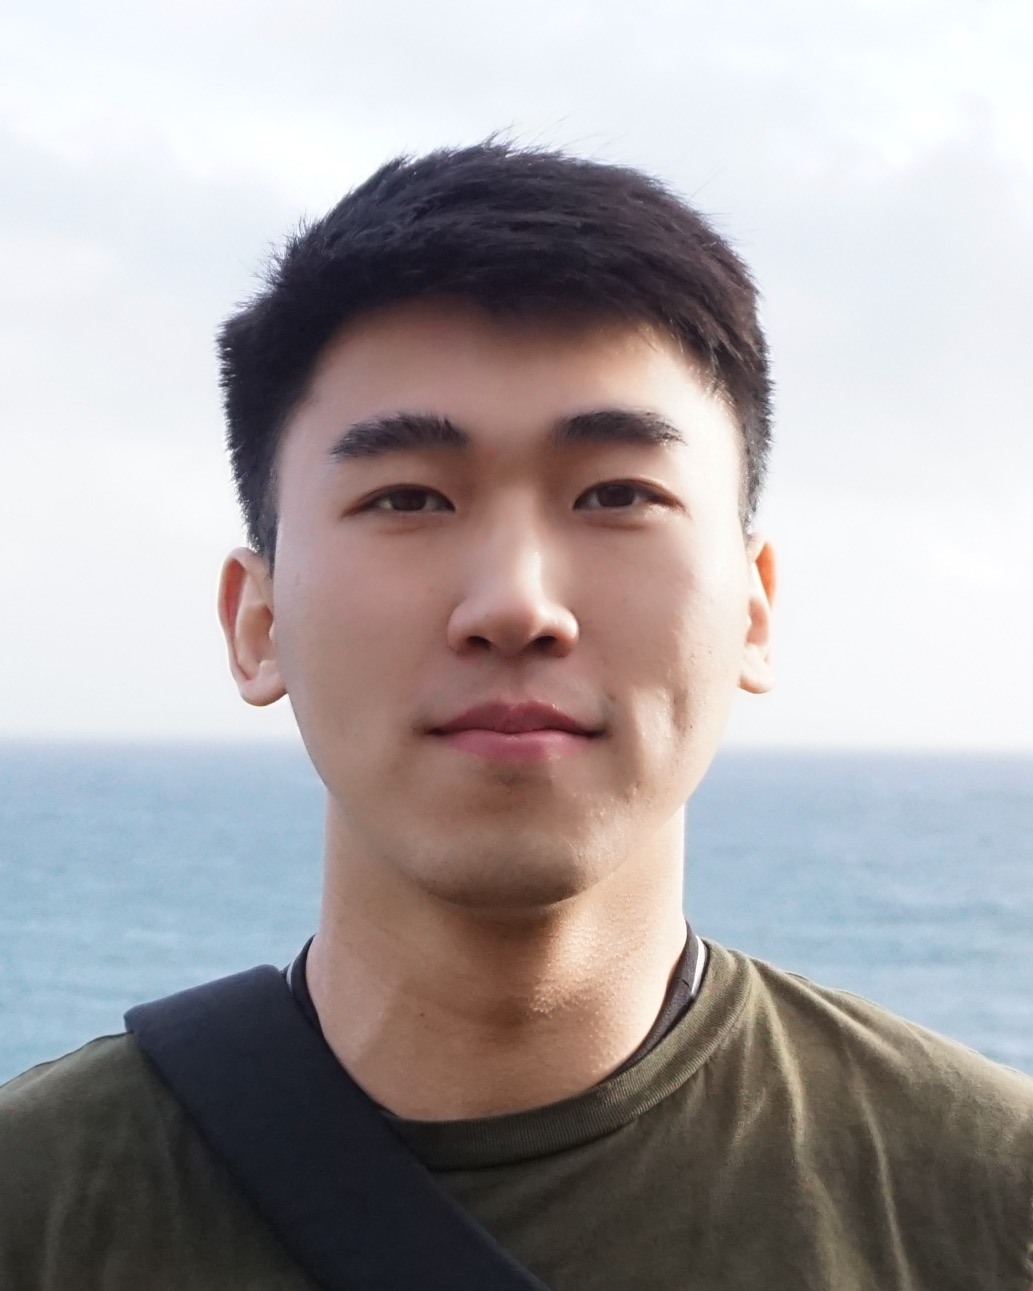
\includegraphics[width=1in,height=1.25in,clip,keepaspectratio]{jiezhan.jpeg}}]{Jie Zhan}
received the B.Eng. degree in electrical engineering from Xiamen University, China, in 2017. He is currently pursuing a Ph.D. in electronic engineering with the School of Electronics and Computer Science, University of Southampton. His research is focused on efficient intermittent computing for batteryless energy-harvesting devices
\end{IEEEbiography}

\vspace{-6\baselineskip}

\begin{IEEEbiography}[{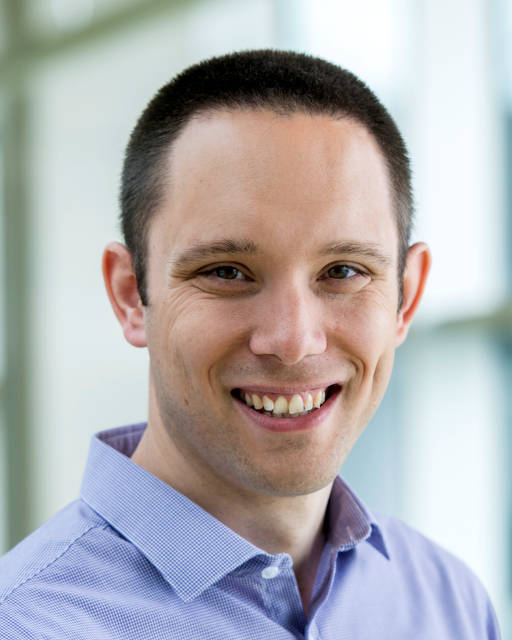
\includegraphics[width=1in,height=1.25in,clip,keepaspectratio]{geoff_merrett_journalbio.jpg}}]{Geoff V. Merrett}

(GSM'06-M'09-SM’19) received the B.Eng. (Hons) and Ph.D. degrees from the University of Southampton, U.K., in 2004 and 2008, respectively. He currently holds a Personal Chair in Electronic and Software Systems at the School of Electronics and Computer Science, University of Southampton, U.K., where he is Head of the Centre for Internet of Things and Pervasive Systems.

Prior to becoming a Professor in 2019, he was a Lecturer and Associate Professor at Southampton from 2009 and 2014 respectively. He is Co-Director of the Arm-ECS Research Centre, an award winning collaboration between the university and Arm Research, Cambridge. His current research interests are in energy management of mobile/embedded systems and self-powered devices, and he has published over 200 journal and conference articles on these topics.
\end{IEEEbiography}
% short bio
% (GSM’06-M’09-SM’19) is Professor of Electronic and Software Systems at the University of Southampton, U.K., where he previously received the B.Eng. (Hons) and Ph.D. degrees in 2004 and 2008, respectively. 
% He is co-director of the Arm-ECS Research Centre, an award winning collaboration between the university and Arm Research, Cambridge. 
% His current research interests are in energy management of mobile/embedded systems and self-powered devices, and he has published over 200 journal and conference articles on these topics.

% additional
% Prof. Merrett was co-editor of the book "Many-Core Computing: Hardware and Software" (IET, 2019), General Chair of EWME 2016 and ENSsys 2013-15, and an Associate Editor for IET CDT and MDPI Sensors. He is a Member of the IET, and a Fellow of the HEA.

\vspace{-6\baselineskip}

\begin{IEEEbiography}[{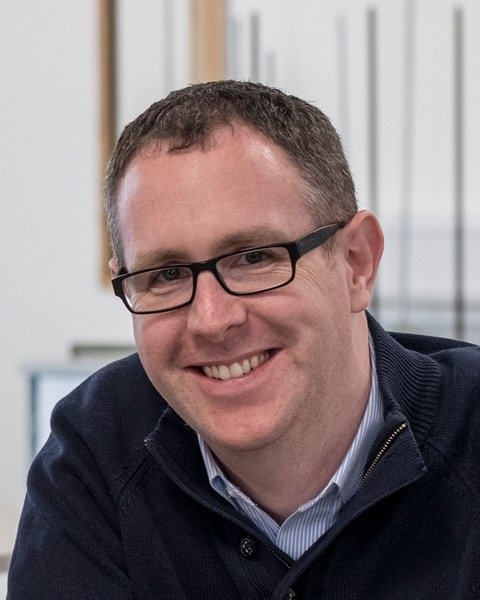
\includegraphics[width=1in,height=1.25in,clip,keepaspectratio]{alex_weddell_journalbio.jpeg}}]{Alex S. Weddell}
(GSM’06-M’10) received the M.Eng. degree (1st class honors) and Ph.D. in electronic engineering from the University of Southampton, U.K., in 2005 and 2010. His main research focus is in the areas of energy harvesting and energy management for future Internet of Things devices.
He has over 15 years’ experience in energy harvesting systems, and has published over 65 papers in the area. 
He is now a Lecturer at the University of Southampton, involved with three projects funded by EPSRC, EU Horizon 2020 and Clean Sky 2.
\end{IEEEbiography}

% insert where needed to balance the two columns on the last page with
% biographies
%\newpage

% You can push biographies down or up by placing
% a \vfill before or after them. The appropriate
% use of \vfill depends on what kind of text is
% on the last page and whether or not the columns
% are being equalized.

%\vfill

% Can be used to pull up biographies so that the bottom of the last one
% is flush with the other column.
%\enlargethispage{-5in}

% \todos

\end{document}